\documentclass{beamer}
\usetheme{testtheme}
\usepackage{graphicx}
\usepackage{subfigure}


\usepackage{textpos}
\setbeamerfont{author in head/foot}{size={\fontsize{3pt}{4pt}\selectfont}}

\setbeamersize{text margin left=2pt,text margin right=2pt}

\author{%
  \makebox[.5\linewidth]{Author 1}\\Affilation 1\\
  \and \makebox[.5\linewidth]{Author 2}\\Affiliation 2\\
  \and \makebox[.5\linewidth]{Author 3}\\Affiliation 3\\
  \and \makebox[.5\linewidth]{Author 4}\\Affiliation 4\\
}




%\maketitle



\title{2L Super-Razor status}
\subtitle{2L/3L EWK Meeting}
\author{dantrim}

\institute{University of California, Irvine}
\date{\today}

\begin{document}




\setcounter{showProgressBar}{0}
	\setcounter{showSlideNumbers}{1}
		\frame{\titlepage}
		
		\begin{frame}
		\frametitle{Contents}
		\begin{enumerate}
			\item Introduction \\ \textcolor{ExecusharesGrey}{\footnotesize\hspace{1em} Testing this theme}
			\item Lorem Text  \\ \textcolor{ExecusharesGrey}{\footnotesize\hspace{1em} Just some Lorem Ipsum for filler}
			\item Conclusions \\ \textcolor{ExecusharesGrey}{\footnotesize\hspace{1em} Some closing thoughts}
		\end{enumerate}
	\end{frame}

		
		
\begin{frame}{Example of columns -- 2 fig column}

	\begin{block}{}
		\begin{columns}[c]
			\column{0.5\paperwidth}
				\centering
				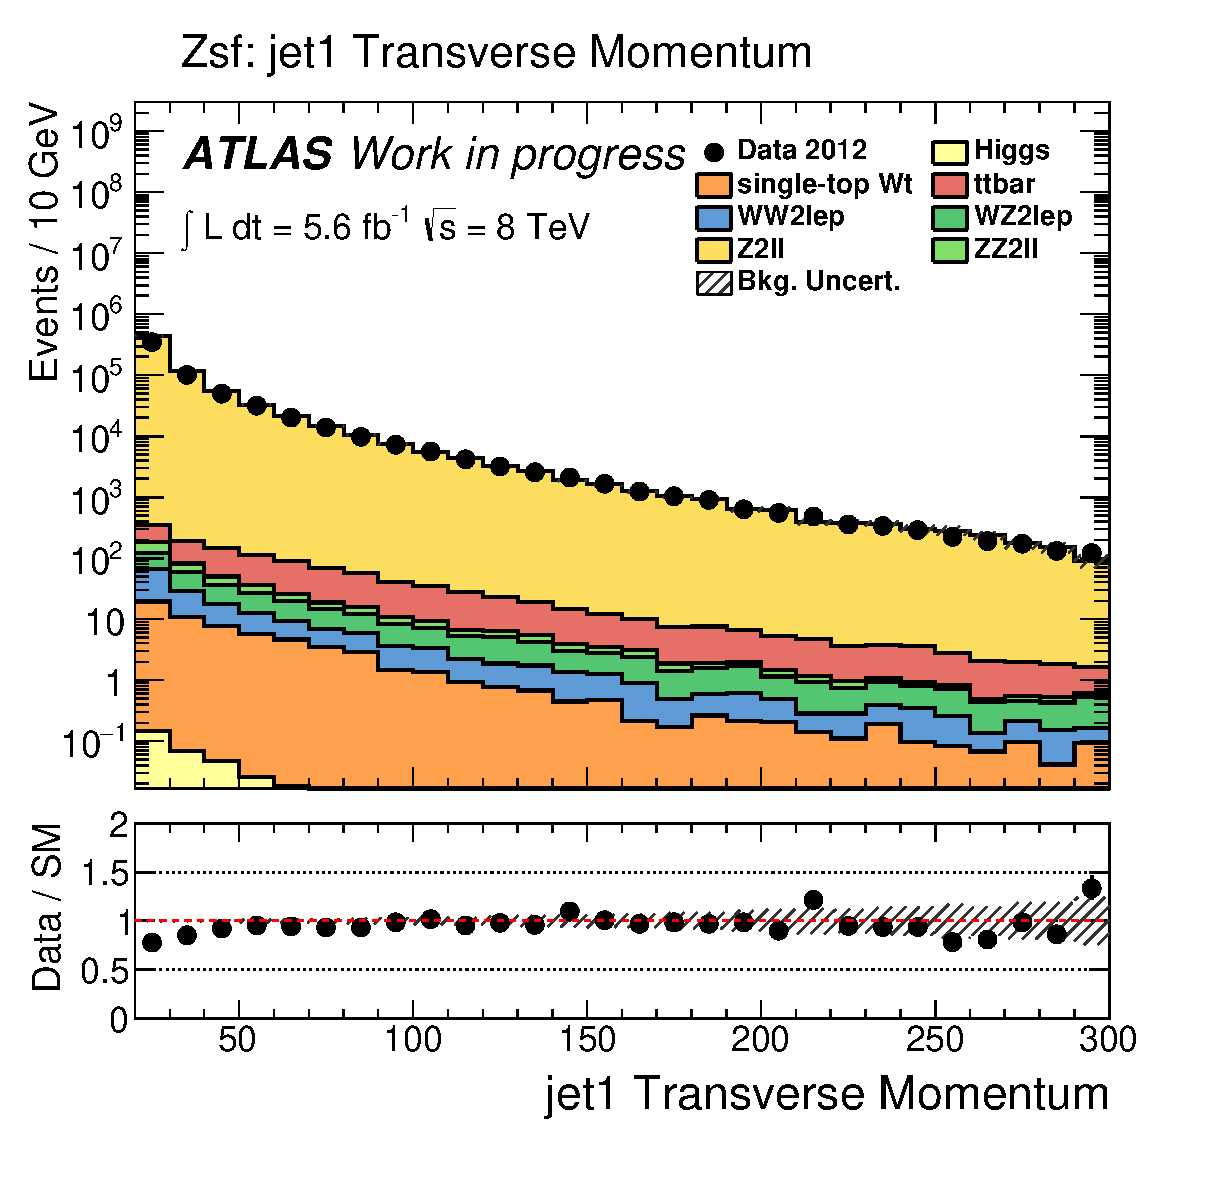
\includegraphics[width=0.65\textwidth]{../scp_landingpad/sf/Zsf_jet1Pt_iso}
			\column{0.5\paperwidth}
				\begin{itemize}
					{\footnotesize
						\item A item
						\item B item
						\item A item
						\item B item
					}
				\end{itemize}	
		\end{columns}
	\end{block}			
	\begin{block}{}
		\begin{columns}[c]
			\column{0.5\paperwidth}
				\centering
				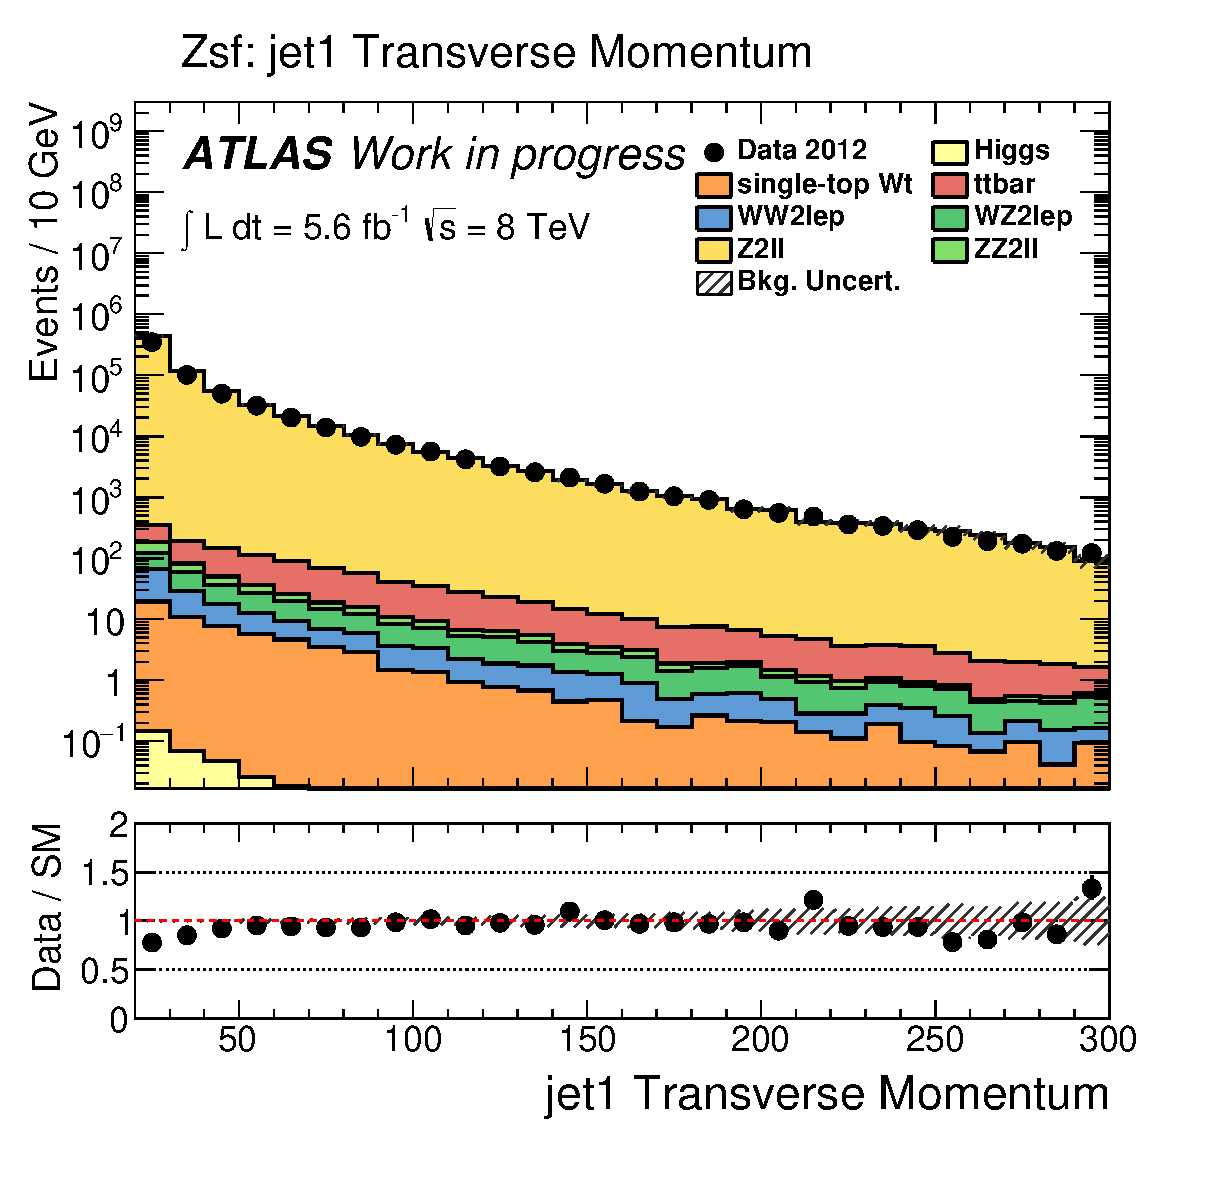
\includegraphics[width=0.65\textwidth]{../scp_landingpad/sf/Zsf_jet1Pt_iso}
			\column{0.5\paperwidth}
				\begin{itemize}
					{\footnotesize
						\item A item
						\item B item
						\item A item
						\item B item
					}
				\end{itemize}	
		\end{columns}
	\end{block}
	
\end{frame}
	
		
		
	
\begin{frame}{Example of columns -- 3 fig (paper width)}

	\begin{block}{}  % for upper row of figures
		\begin{columns}[c]
		%	\centering
			\column{0.33\paperwidth}
				\centering
				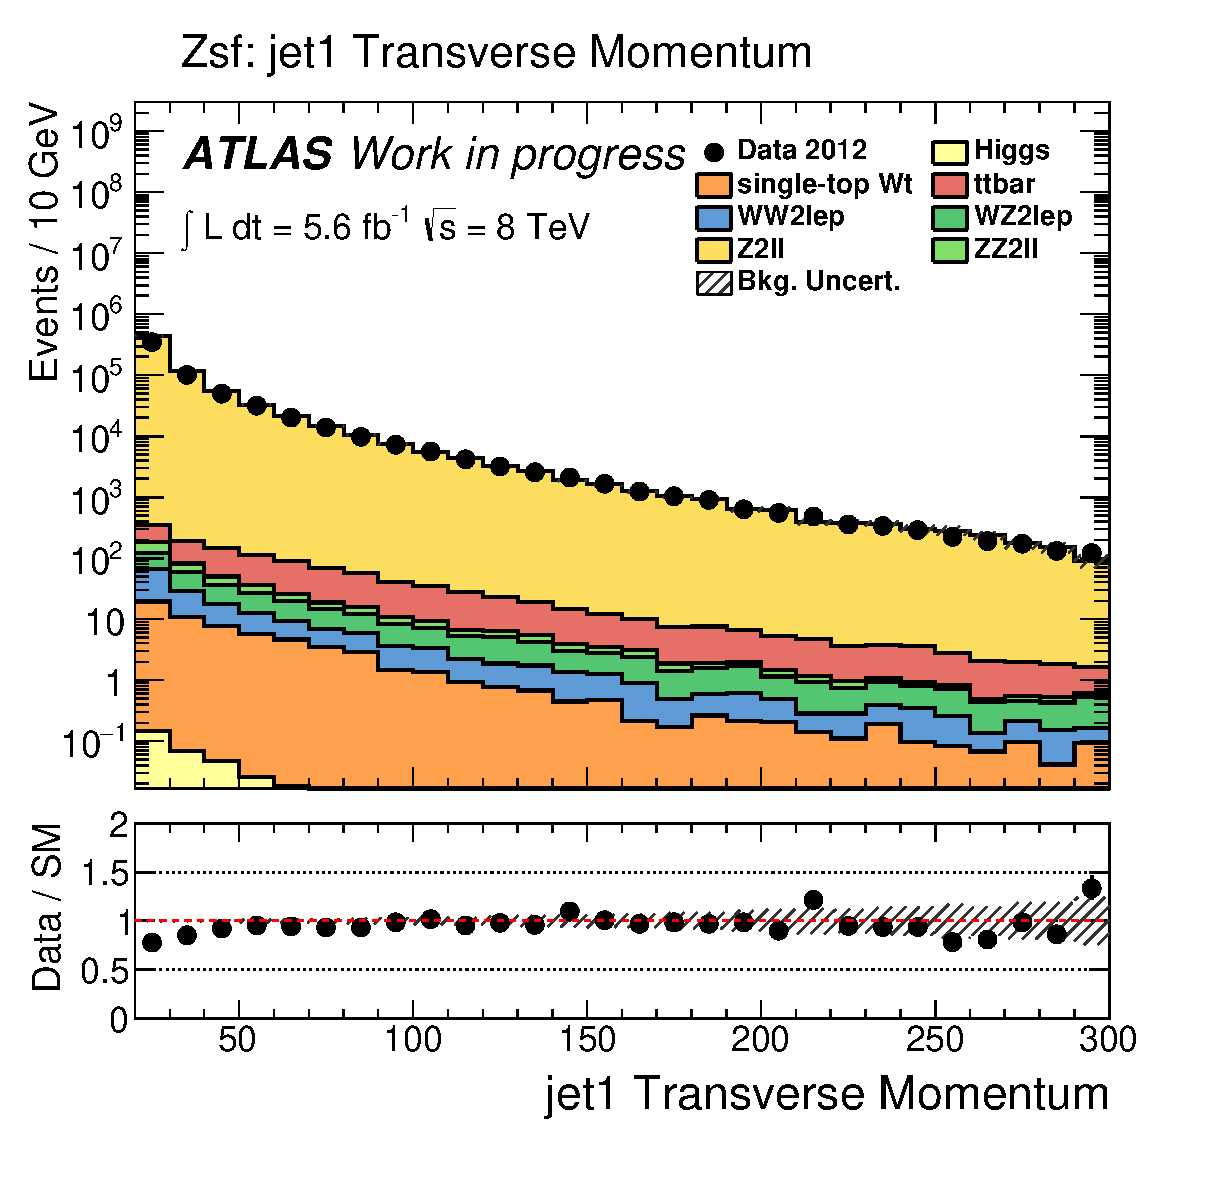
\includegraphics[width=0.95\textwidth]{../scp_landingpad/sf/Zsf_jet1Pt_iso}
			\column{0.33\paperwidth}
				\centering
				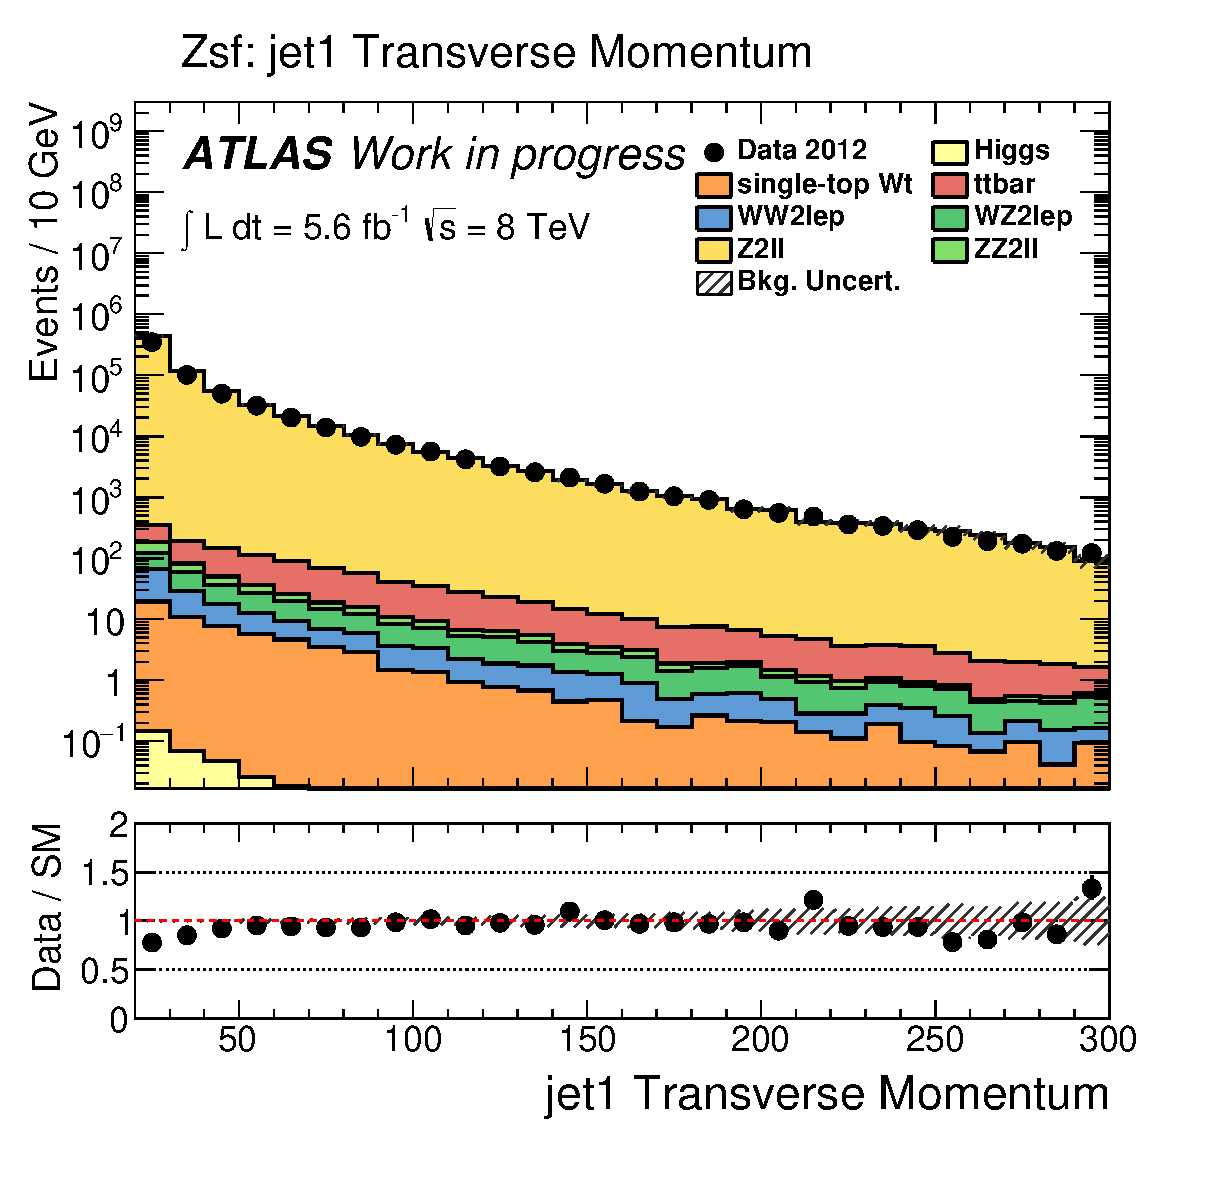
\includegraphics[width=0.95\textwidth]{../scp_landingpad/sf/Zsf_jet1Pt_iso}
			\column{0.33\paperwidth}
				\centering
				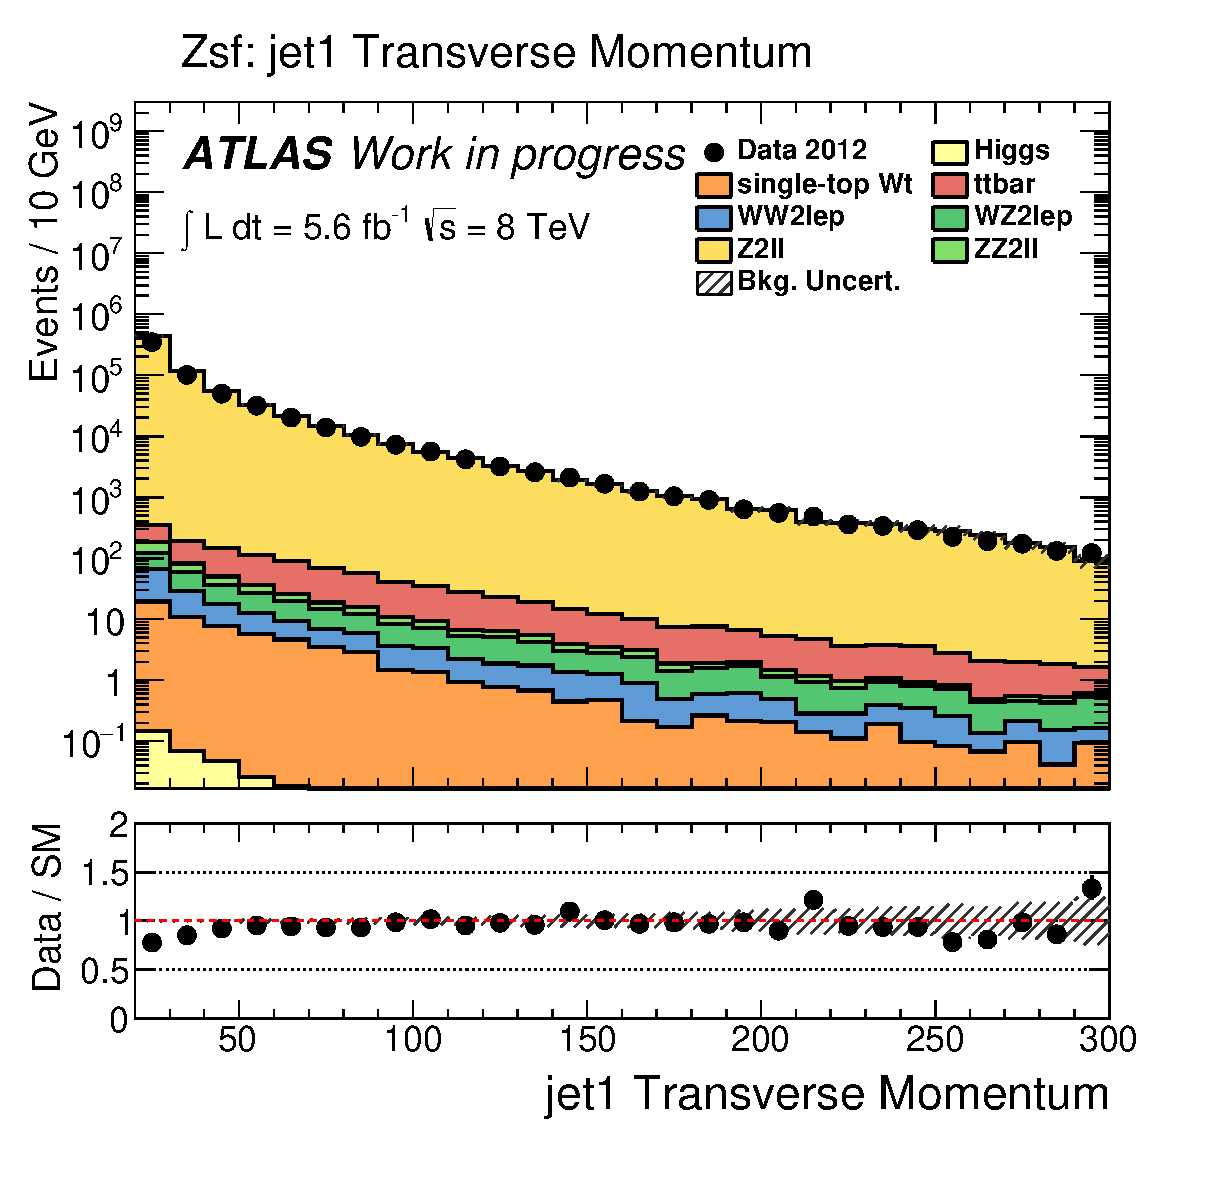
\includegraphics[width=0.95\textwidth]{../scp_landingpad/sf/Zsf_jet1Pt_iso}

				%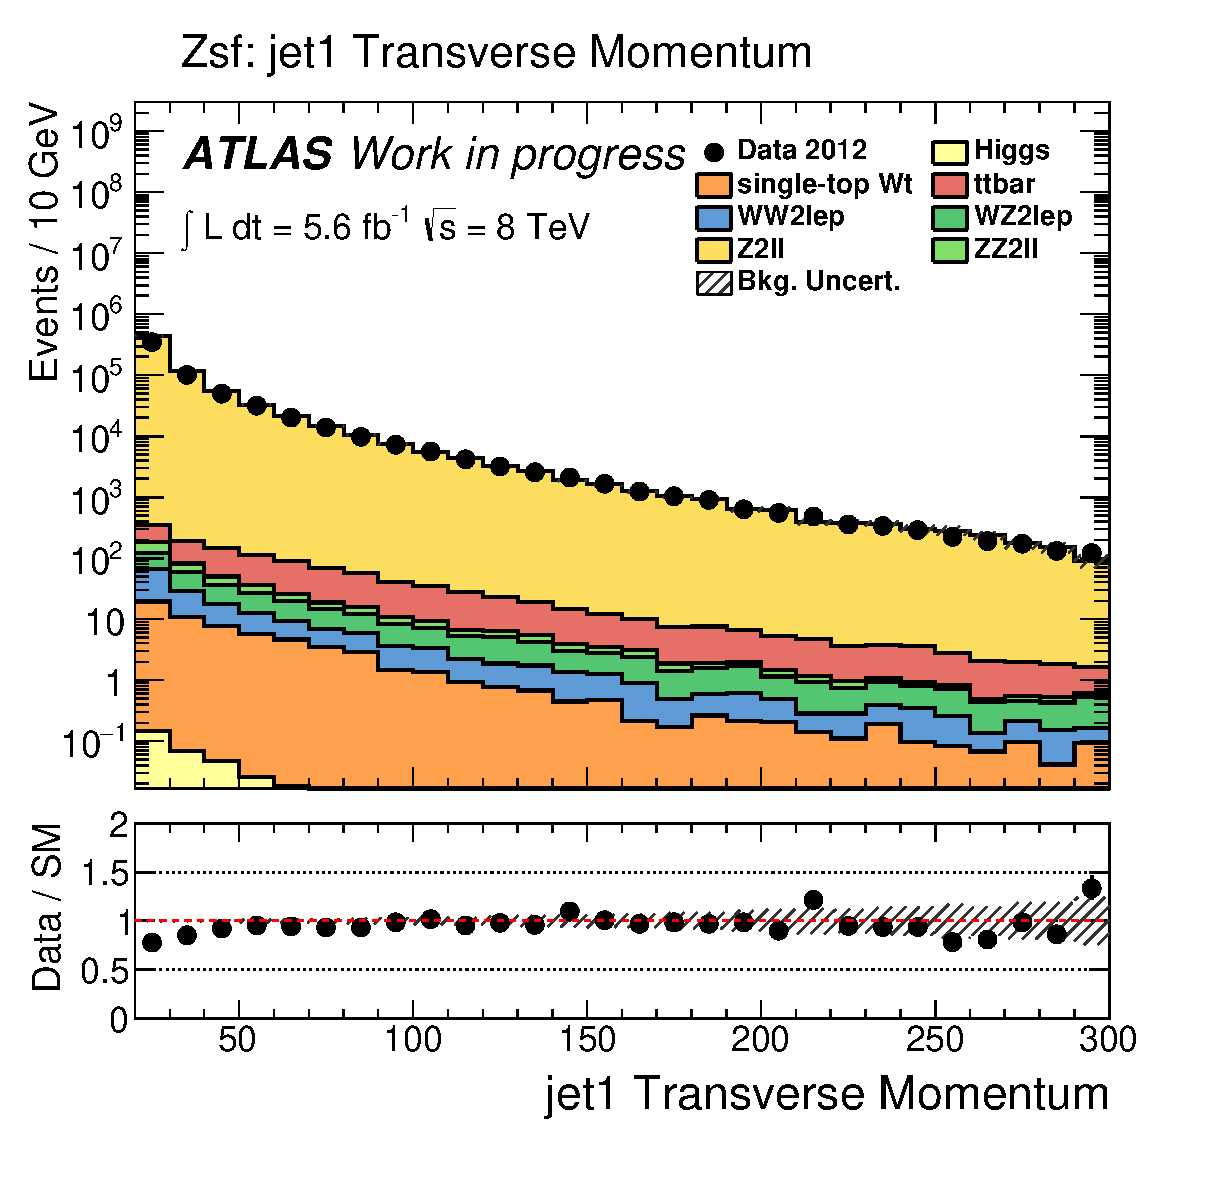
\includegraphics[width=1.2\textwidth]{../scp_landingpad/sf/Zsf_jet1Pt_iso}
		%	\end{column}
%			\begin{column}[T]{3cm}
%				\centering
%				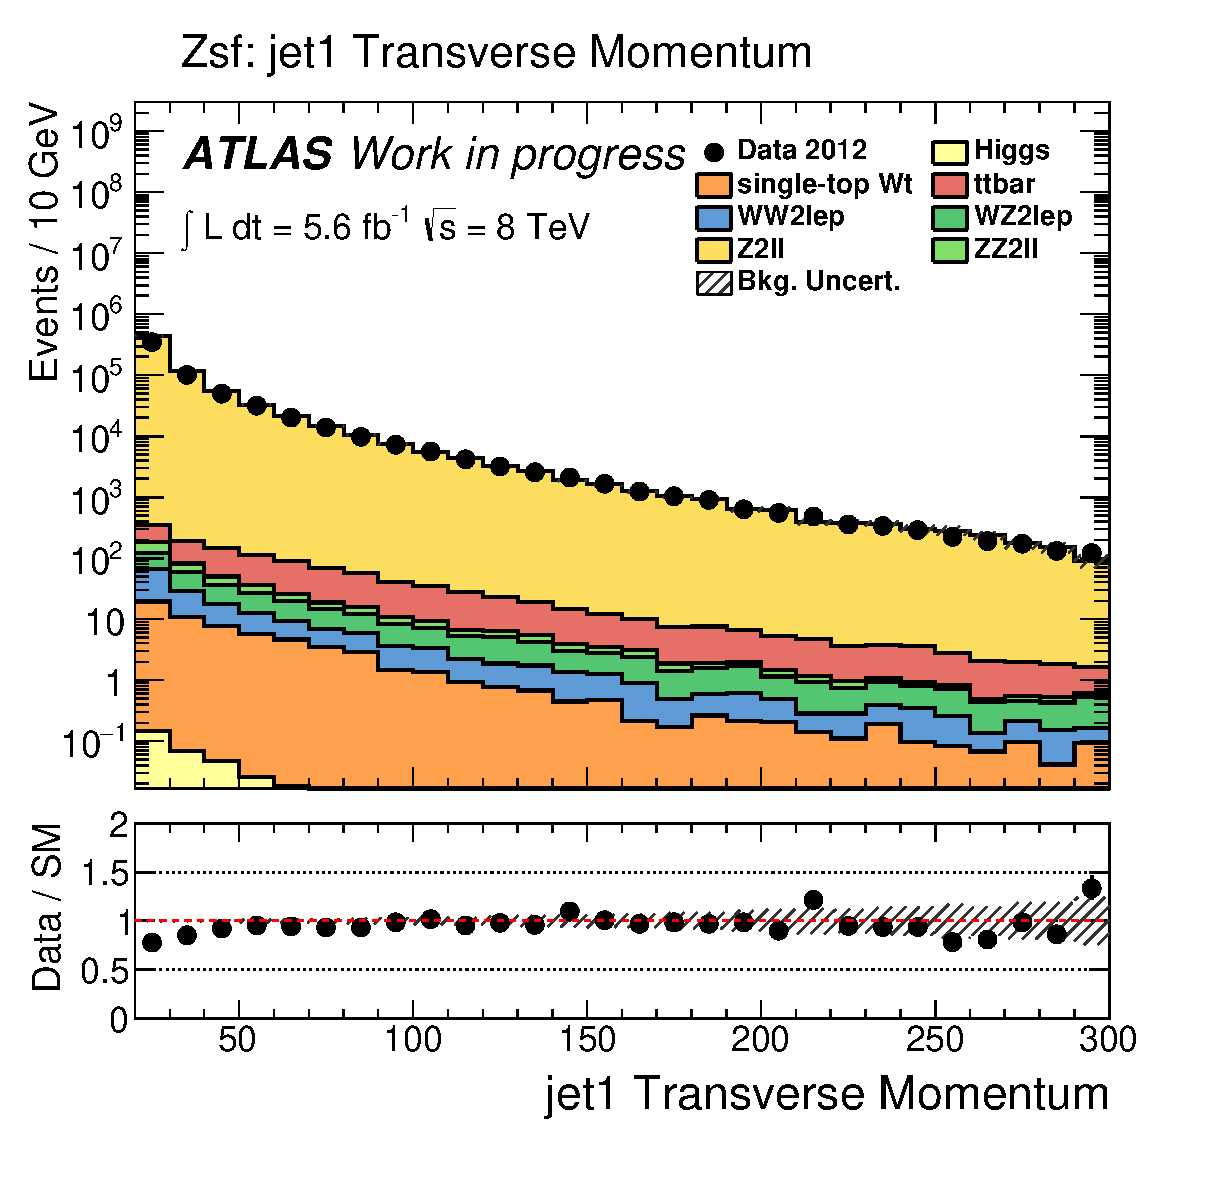
\includegraphics[height=3cm]{../scp_landingpad/sf/Zsf_jet1Pt_iso}
%			%					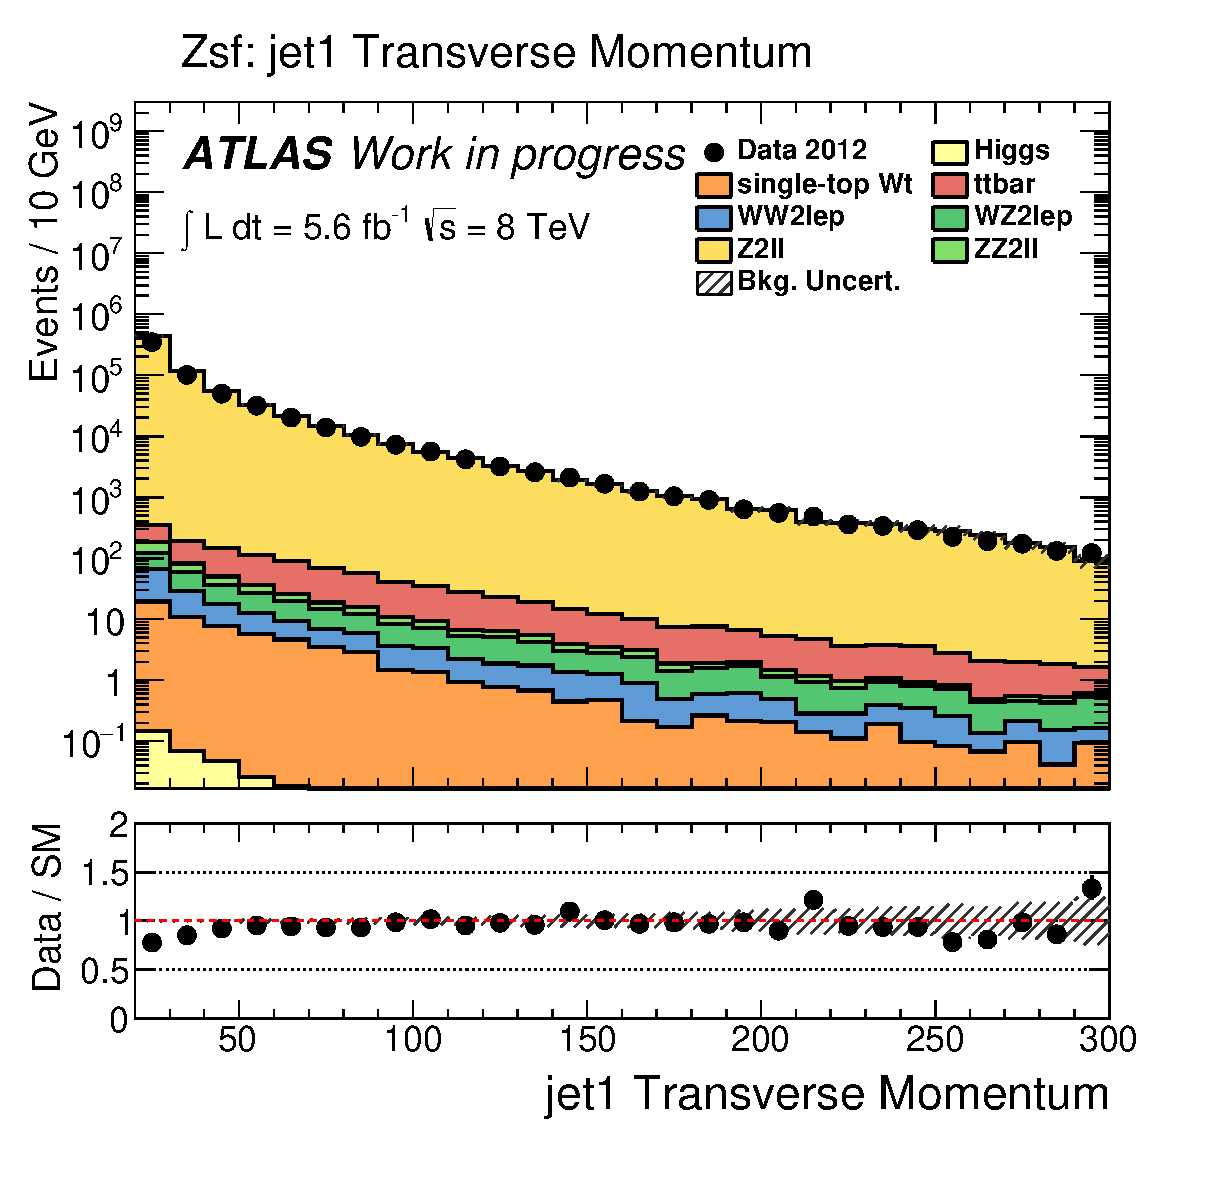
\includegraphics[width=1.2\textwidth]{../scp_landingpad/sf/Zsf_jet1Pt_iso}
%			\end{column}
%			\begin{column}[T]{3cm}
%				\centering
%				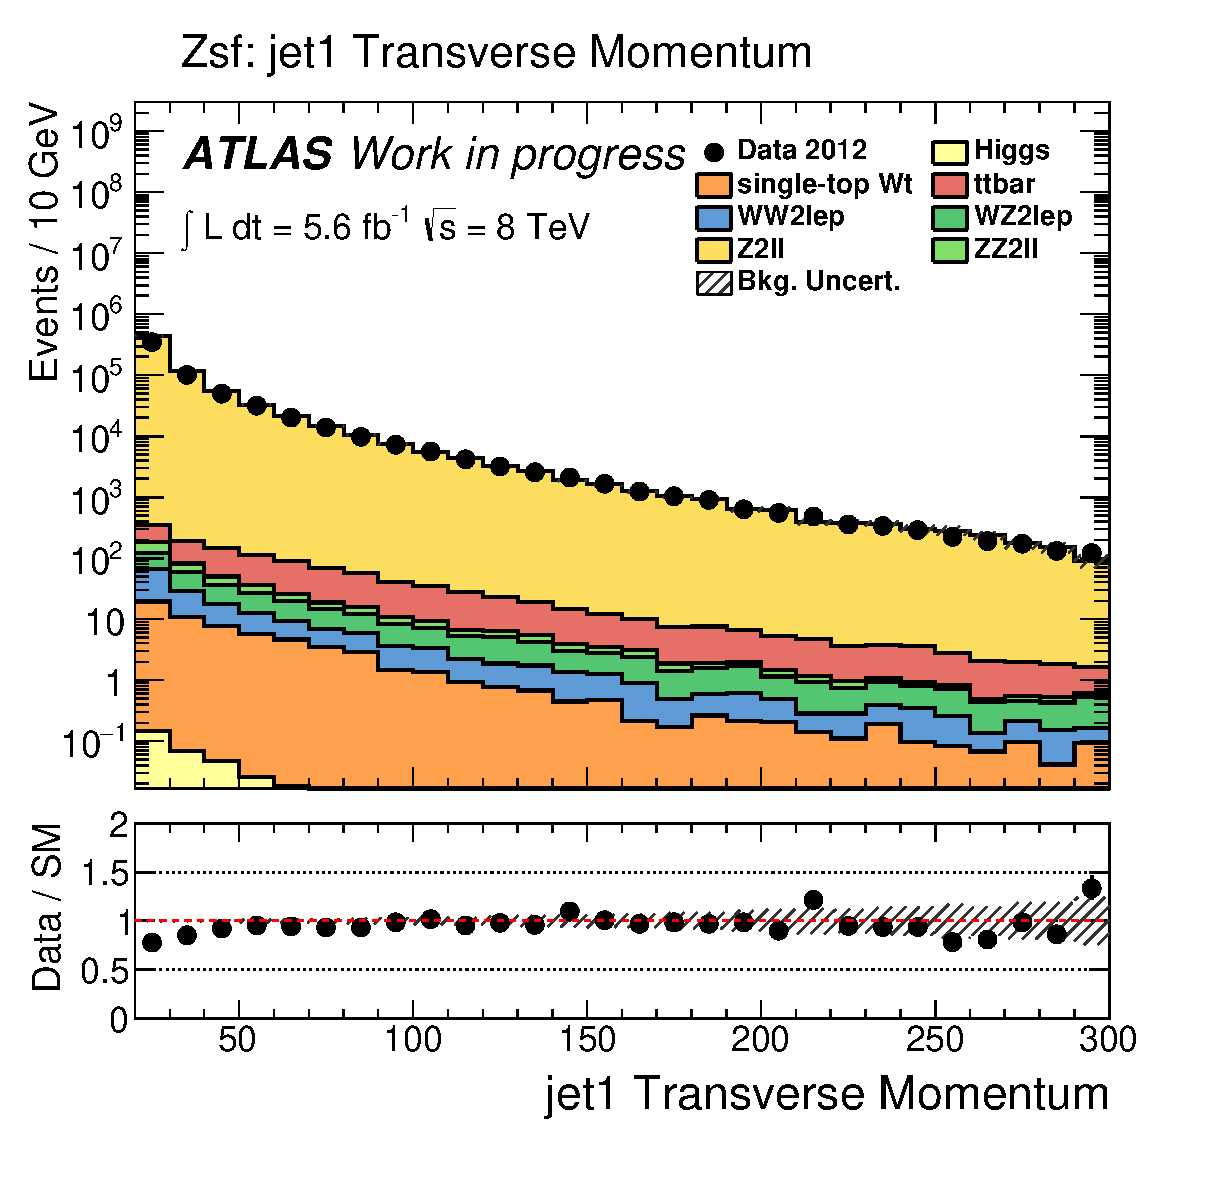
\includegraphics[height=3cm]{../scp_landingpad/sf/Zsf_jet1Pt_iso}
%			%					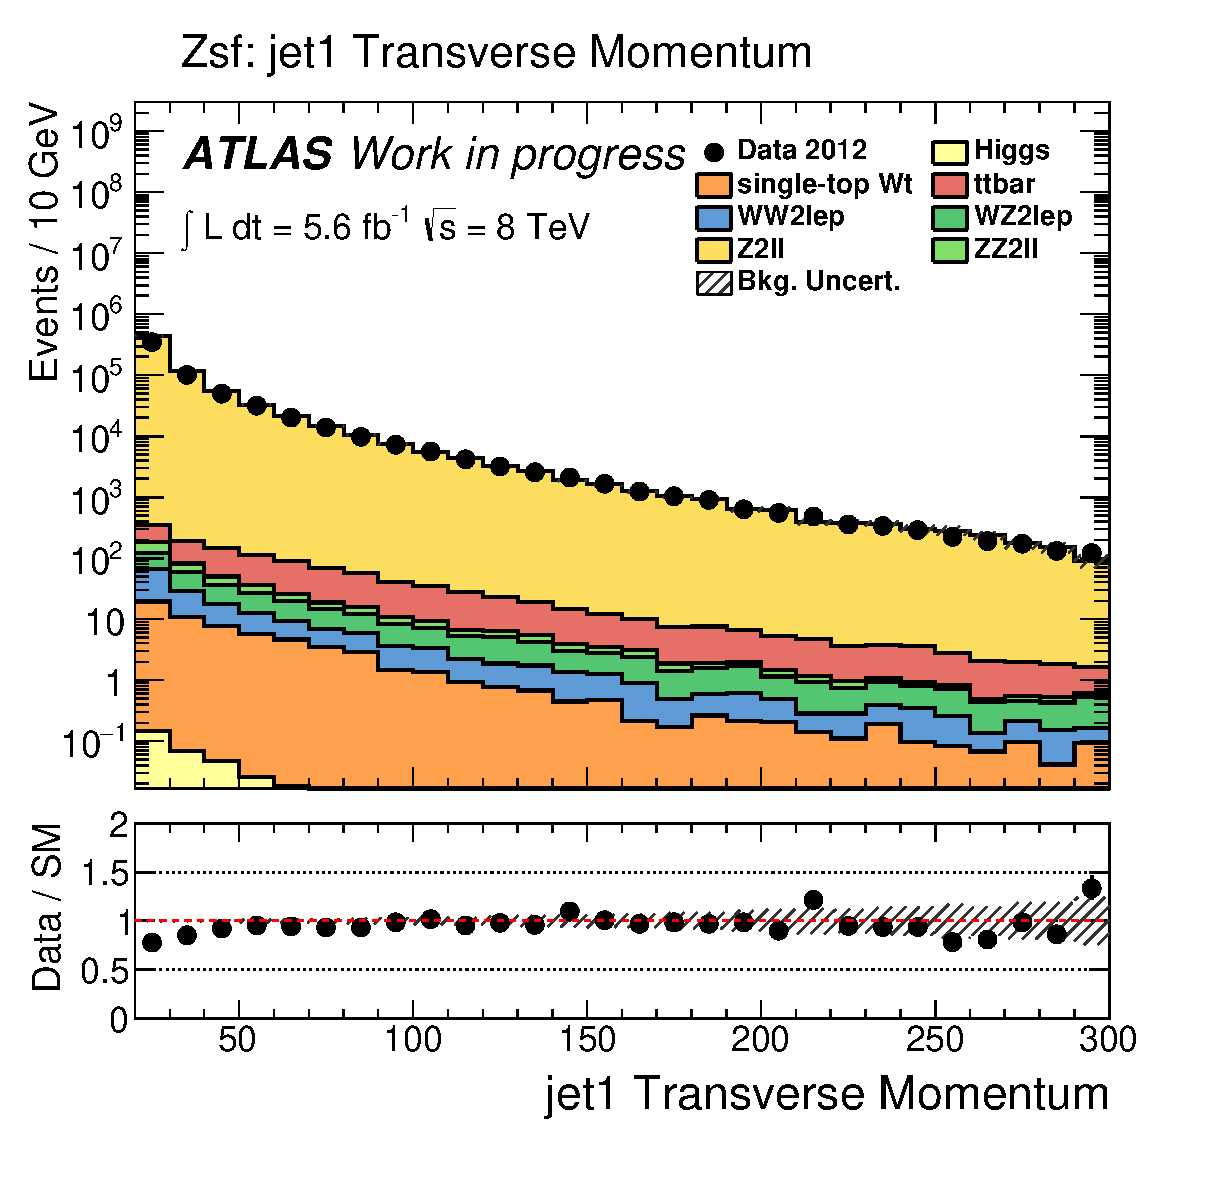
\includegraphics[width=1.2\textwidth]{../scp_landingpad/sf/Zsf_jet1Pt_iso}
%			\end{column}
		\end{columns}


	\end{block}
	\begin{block}{} % lower row of text
		\begin{itemize}
			{\footnotesize
			\item As can be seen, TightLLH may be less preferable than MediumLLH in terms of S/$\sqrt{B}$  \\ \textcolor{ExecusharesGrey}{\tiny\hspace{1em} The reasoning and background behind this theme}  \\ \textcolor{ExecusharesGrey}{\tiny\hspace{1em} The reasoning and background behind this theme}
			\item This must be looked into as the development of the signal region continues
			\item As can be seen, TightLLH may be less preferable than MediumLLH in terms of S/$\sqrt{B}$
			\item This must be looked into as the development of the signal region continues
		}
		\end{itemize}
	\end{block}
		\end{frame}
		
		
\begin{frame}{Example of columns -- 2 fig}

	\begin{block}{}  % for upper row of figures
		\begin{columns}[c]
		%	\centering
			\column{0.5\paperwidth}
				\centering
				%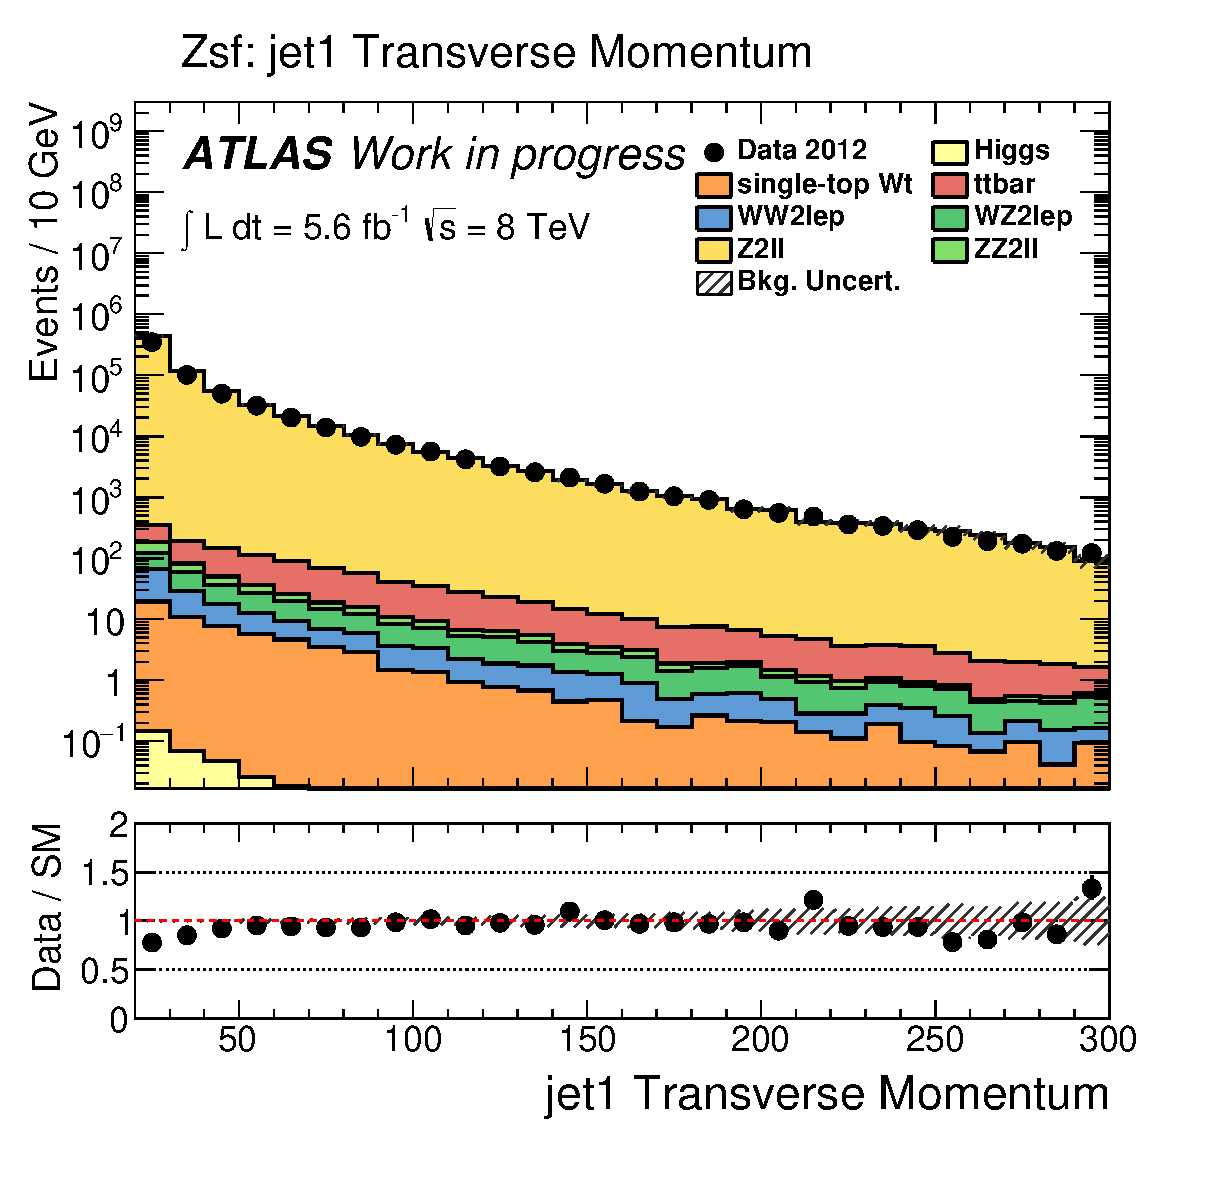
\includegraphics[height=4cm]{../scp_landingpad/sf/Zsf_jet1Pt_iso}
				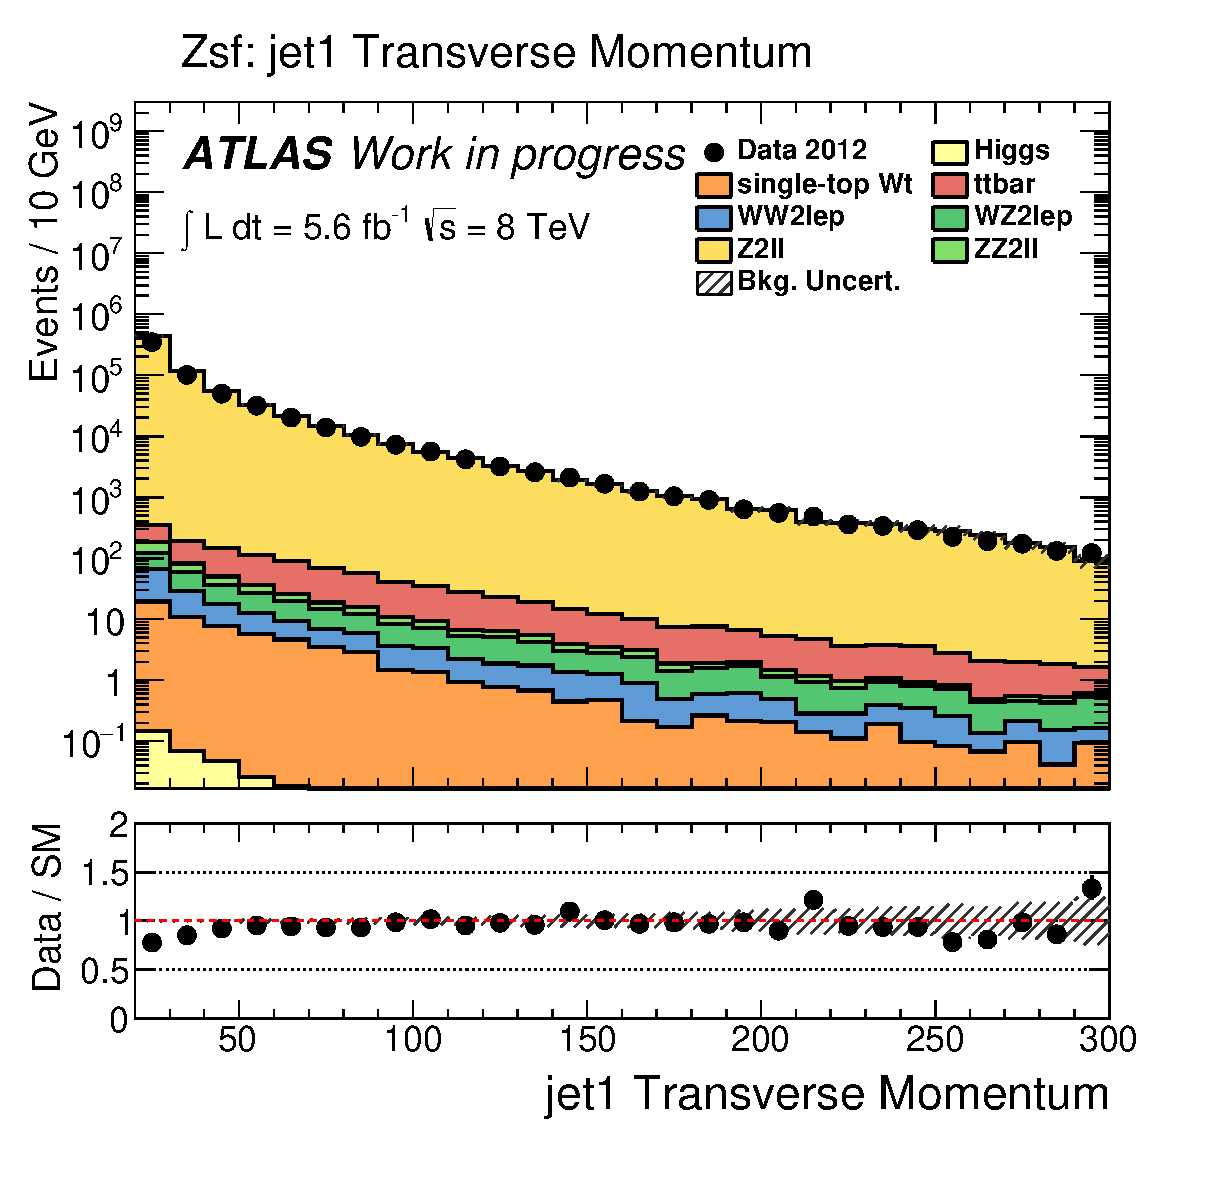
\includegraphics[width=0.8\textwidth]{../scp_landingpad/sf/Zsf_jet1Pt_iso}
			\column{0.5\paperwidth}
				\centering
				%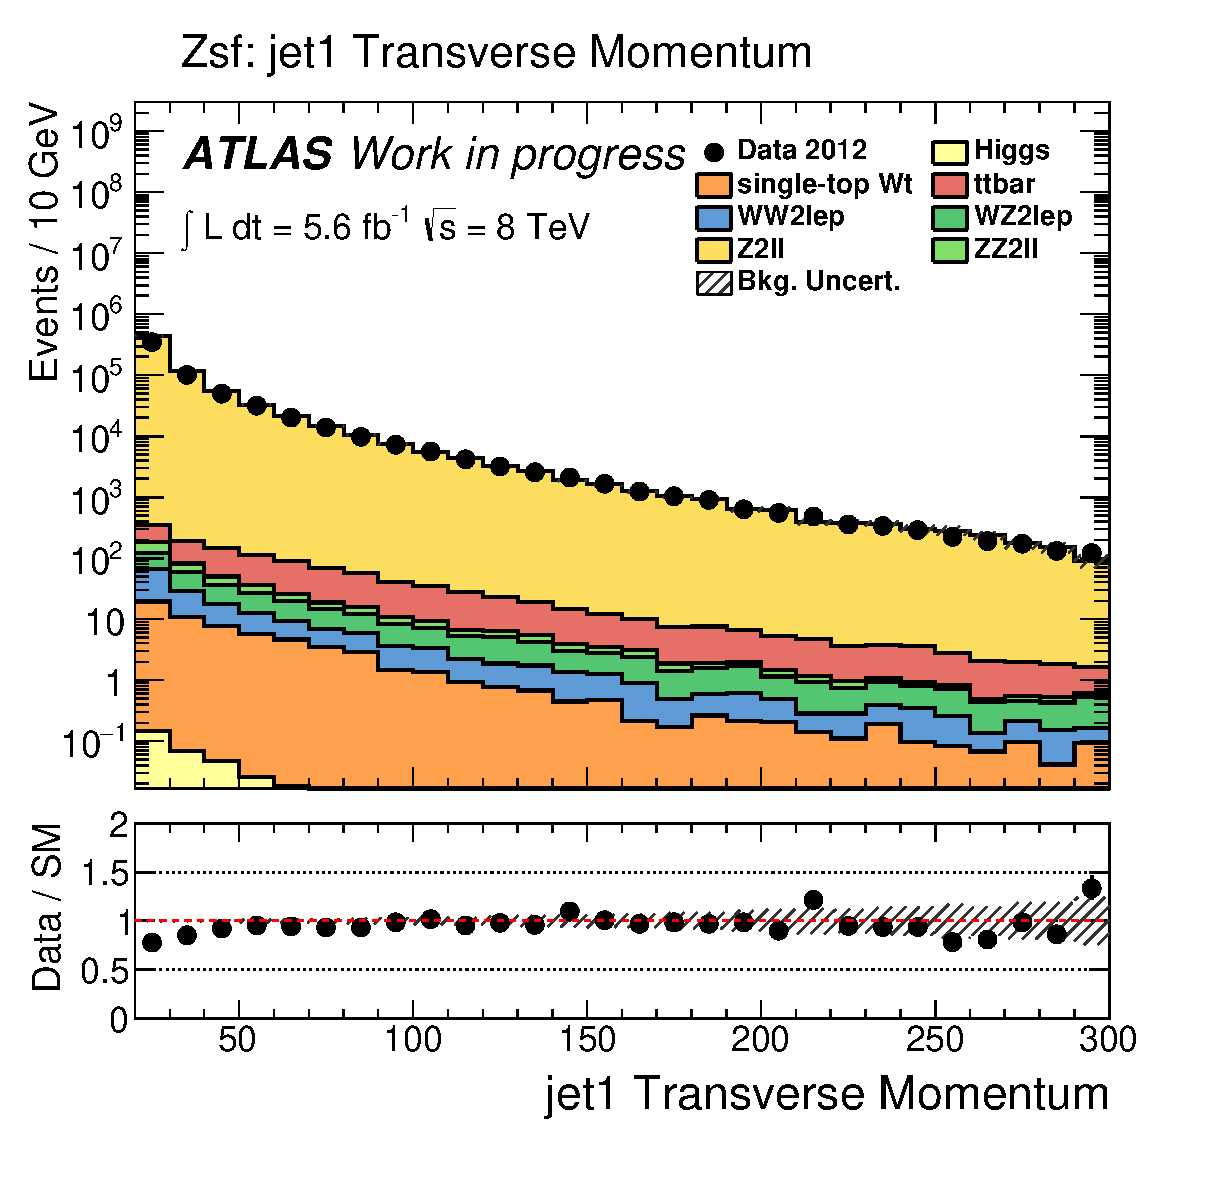
\includegraphics[height=4cm]{../scp_landingpad/sf/Zsf_jet1Pt_iso}
				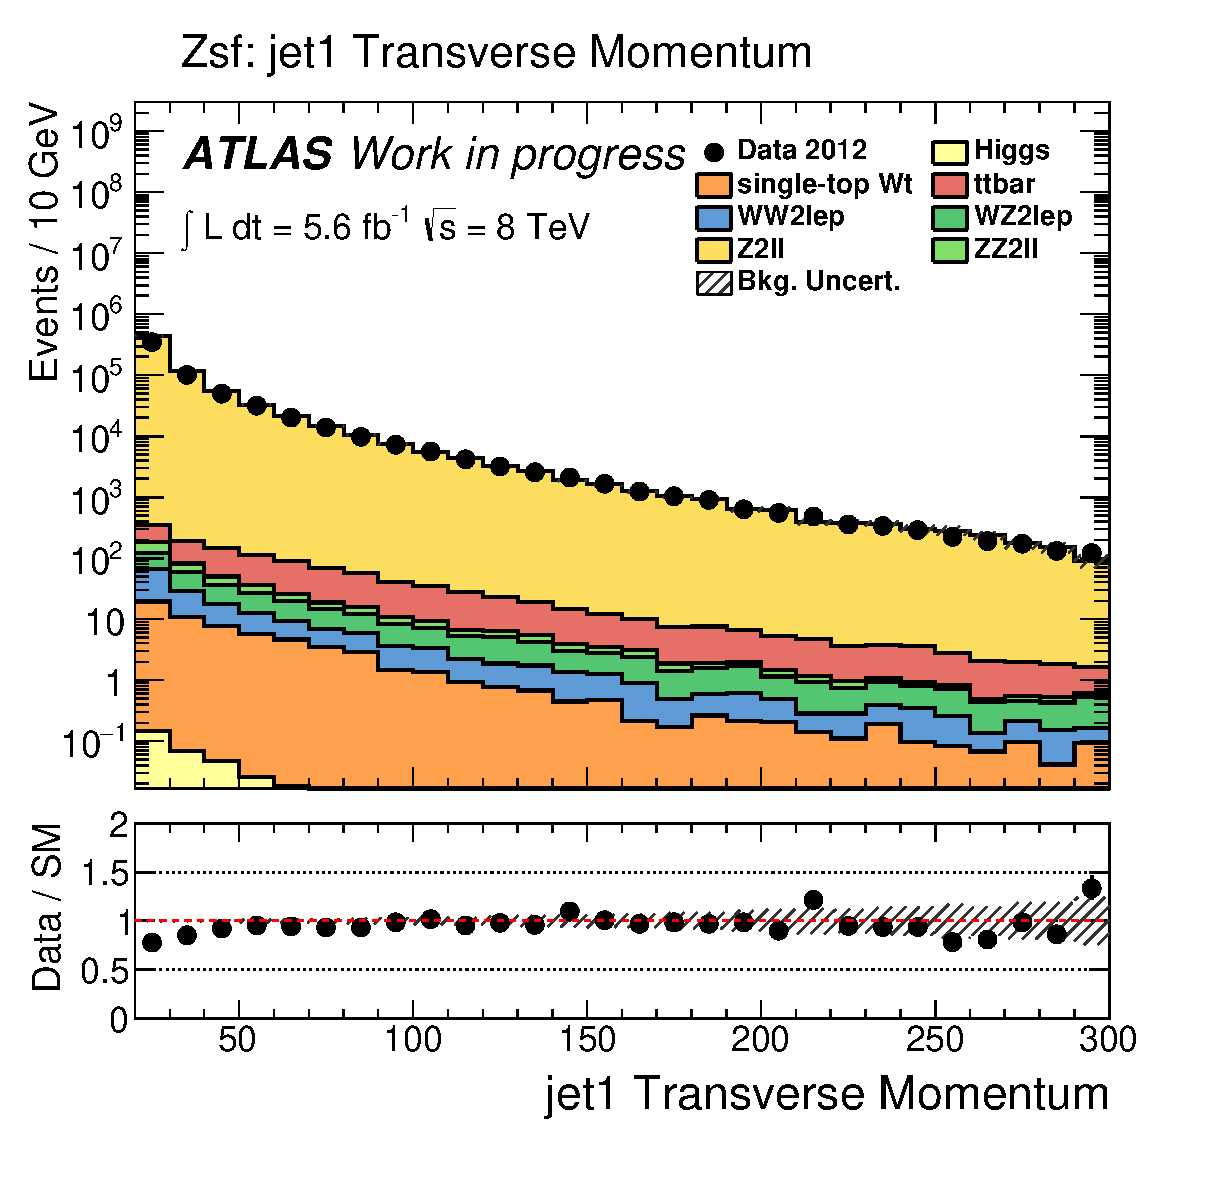
\includegraphics[width=0.8\textwidth]{../scp_landingpad/sf/Zsf_jet1Pt_iso}
			%	\centering
				%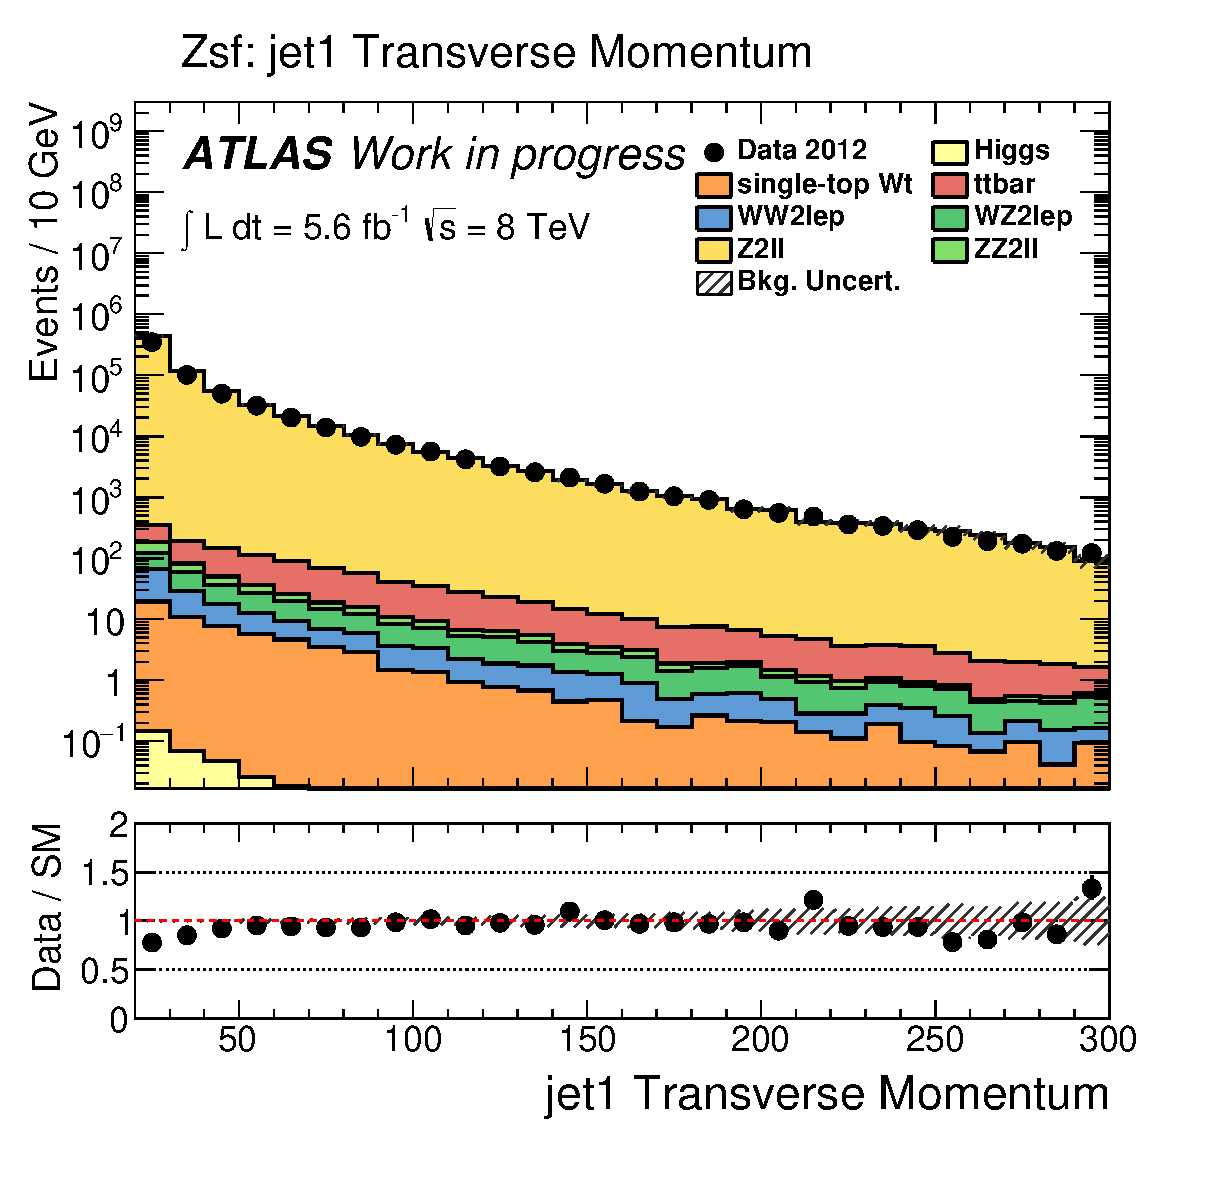
\includegraphics[width=1.2\textwidth]{../scp_landingpad/sf/Zsf_jet1Pt_iso}
		%	\end{column}
%			\begin{column}[T]{3cm}
%				\centering
%				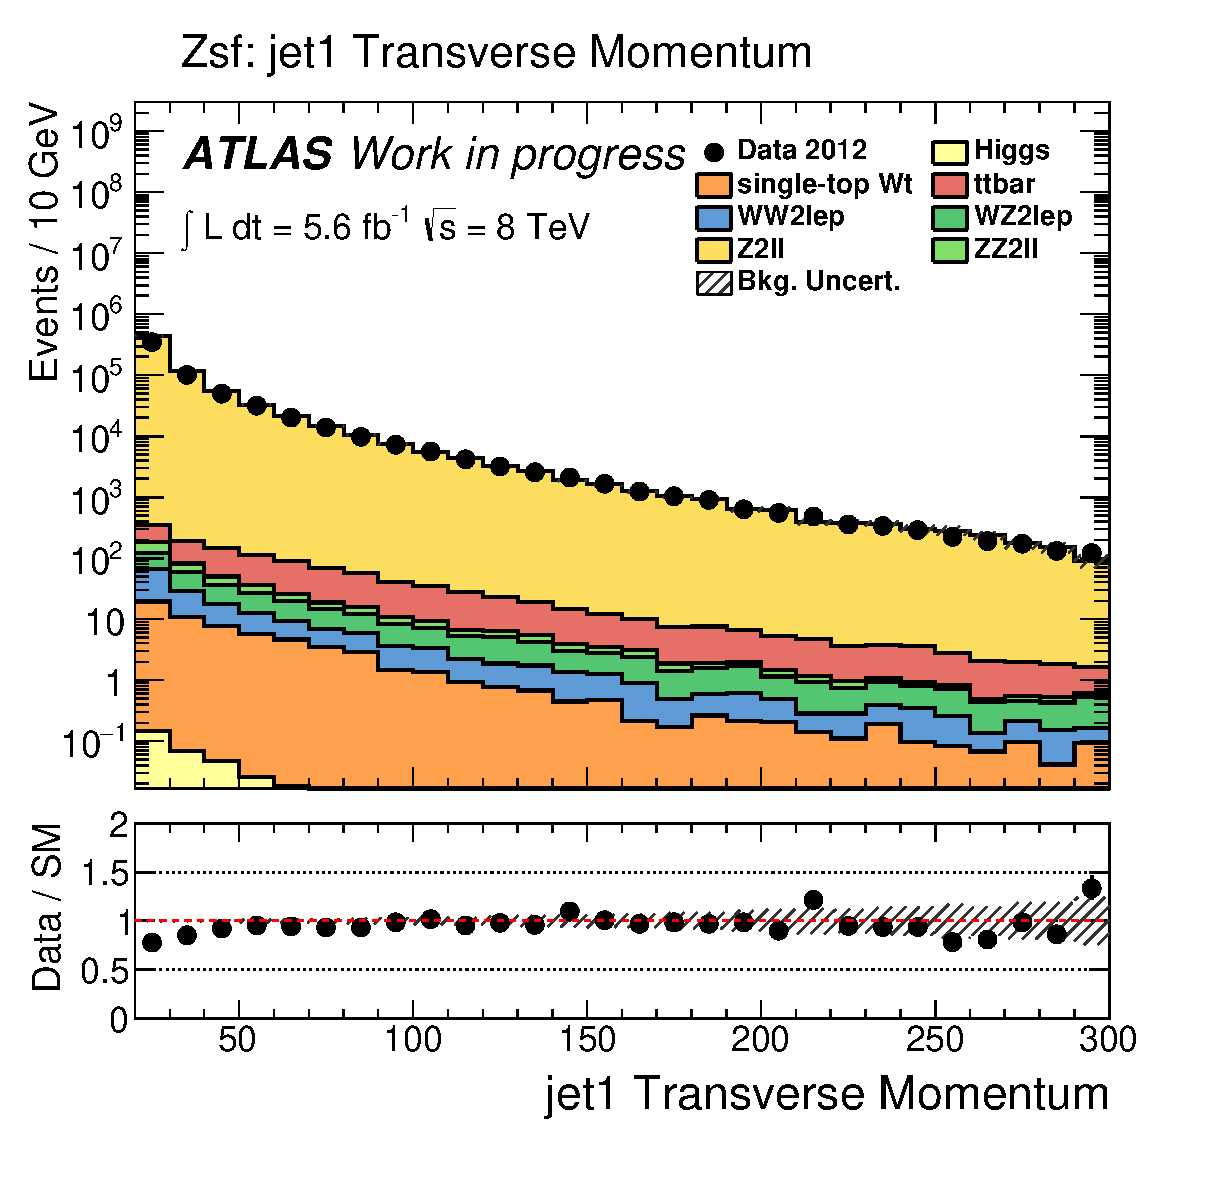
\includegraphics[height=3cm]{../scp_landingpad/sf/Zsf_jet1Pt_iso}
%			%					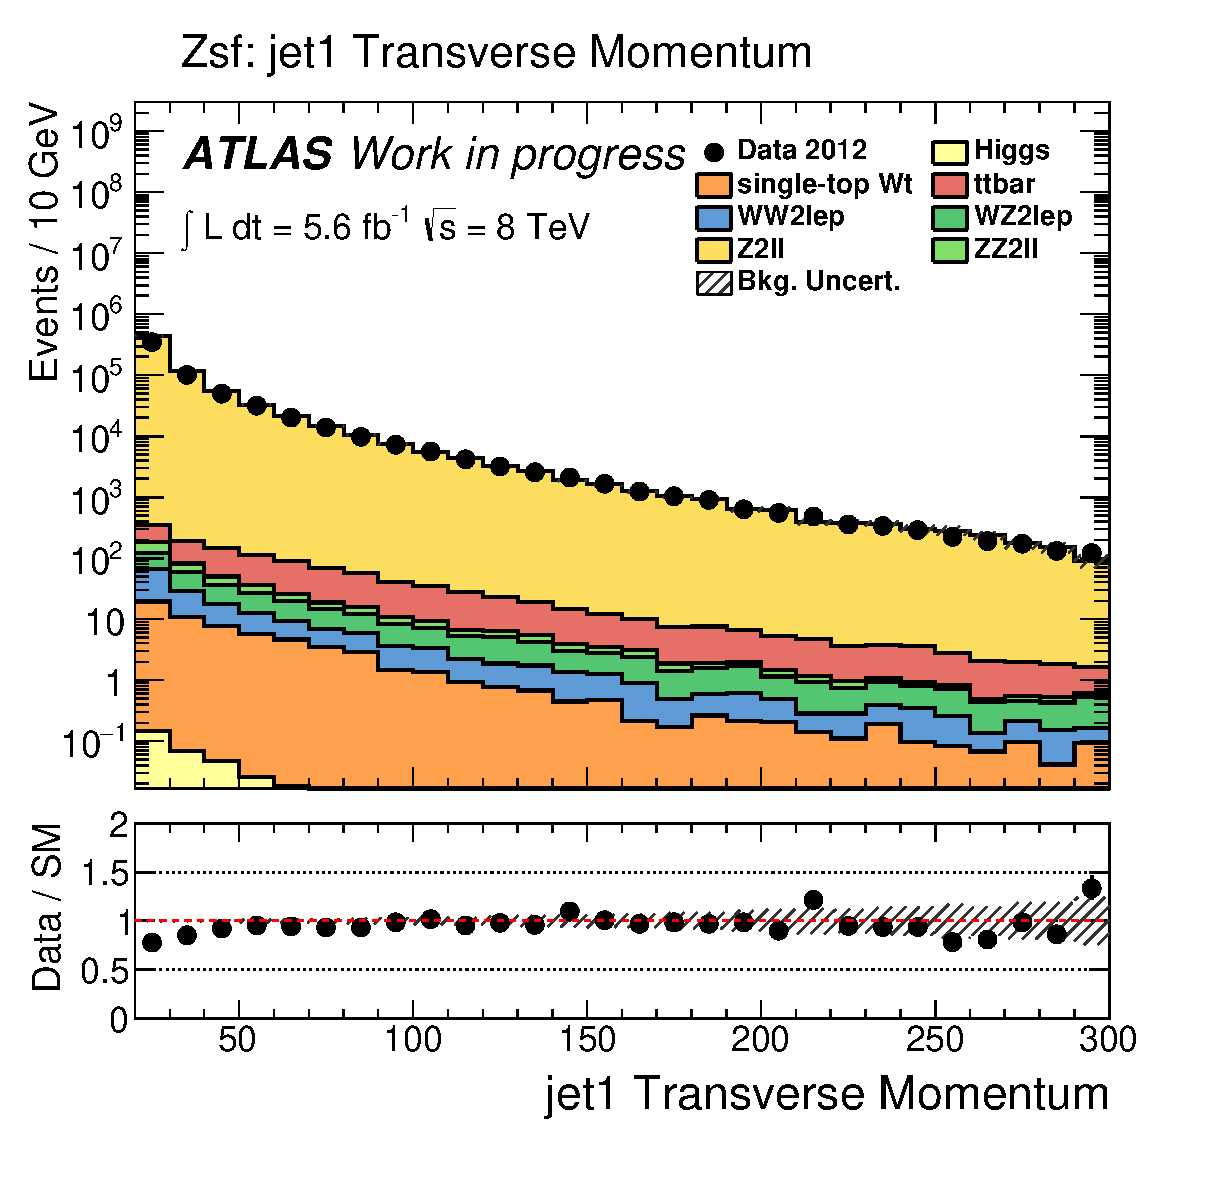
\includegraphics[width=1.2\textwidth]{../scp_landingpad/sf/Zsf_jet1Pt_iso}
%			\end{column}
%			\begin{column}[T]{3cm}
%				\centering
%				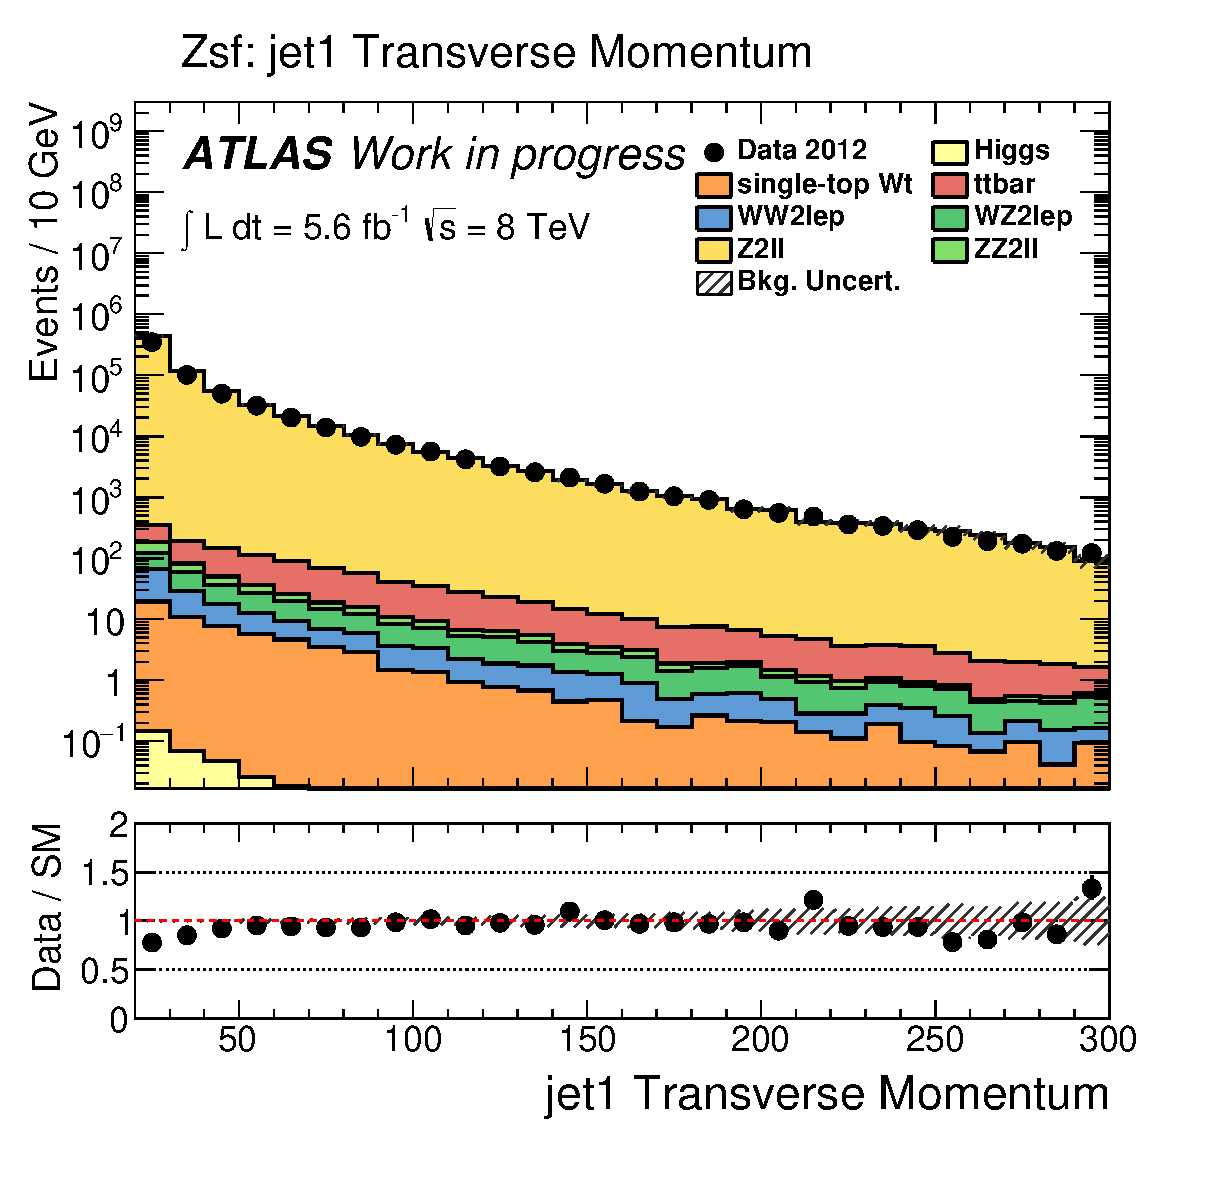
\includegraphics[height=3cm]{../scp_landingpad/sf/Zsf_jet1Pt_iso}
%			%					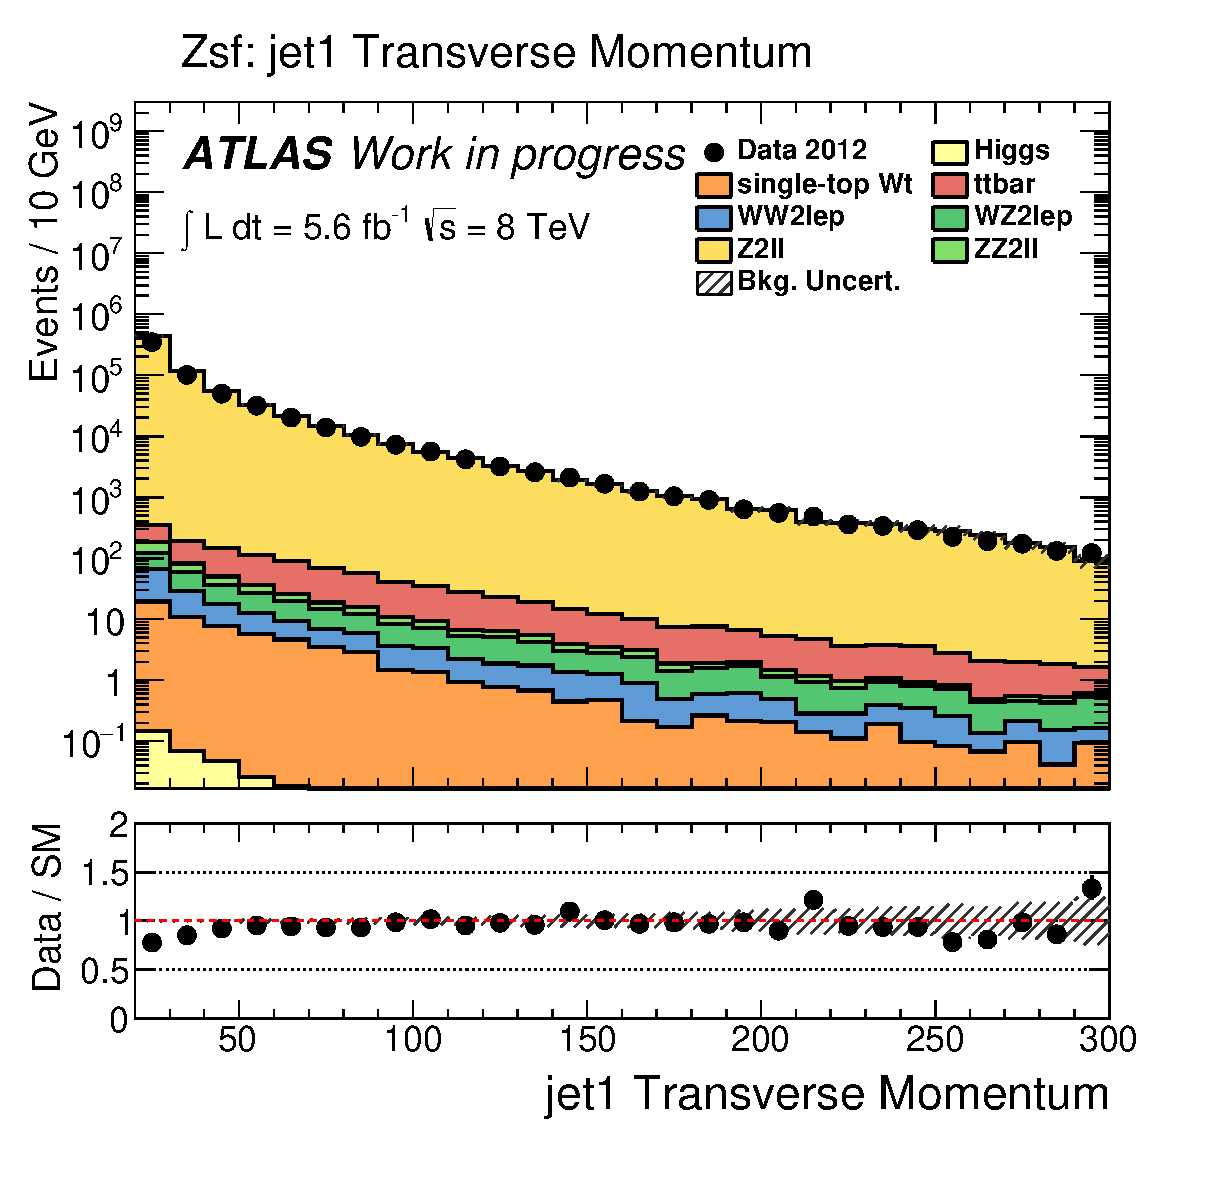
\includegraphics[width=1.2\textwidth]{../scp_landingpad/sf/Zsf_jet1Pt_iso}
%			\end{column}
		\end{columns}


	\end{block}
	\begin{block}{} % lower row of text
		\begin{itemize}
			\item As can be seen, TightLLH may be less preferable than MediumLLH in terms of S/$\sqrt{B}$
			\item This must be looked into as the development of the signal region continues
		\end{itemize}
	\end{block}
		\end{frame}
		
		
		
\begin{frame}{Example of columns -- 4 fig}

	\begin{block}{}  % for upper row of figures
		\begin{columns}[c]
		%	\centering
			\column{0.4\paperwidth}
				\centering
				%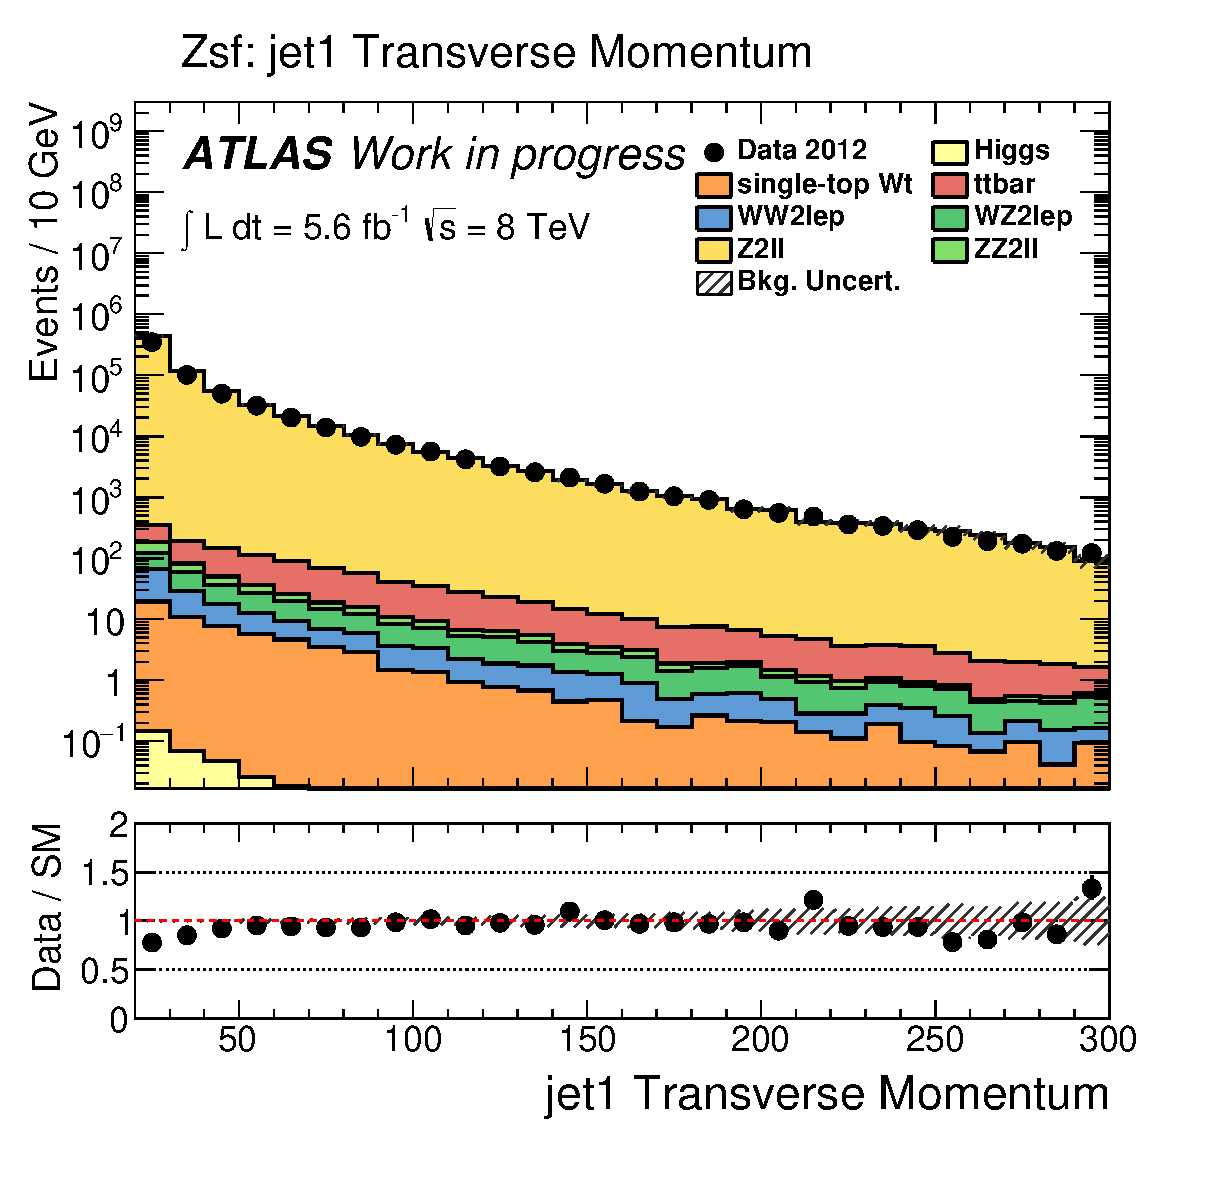
\includegraphics[height=4cm]{../scp_landingpad/sf/Zsf_jet1Pt_iso}
				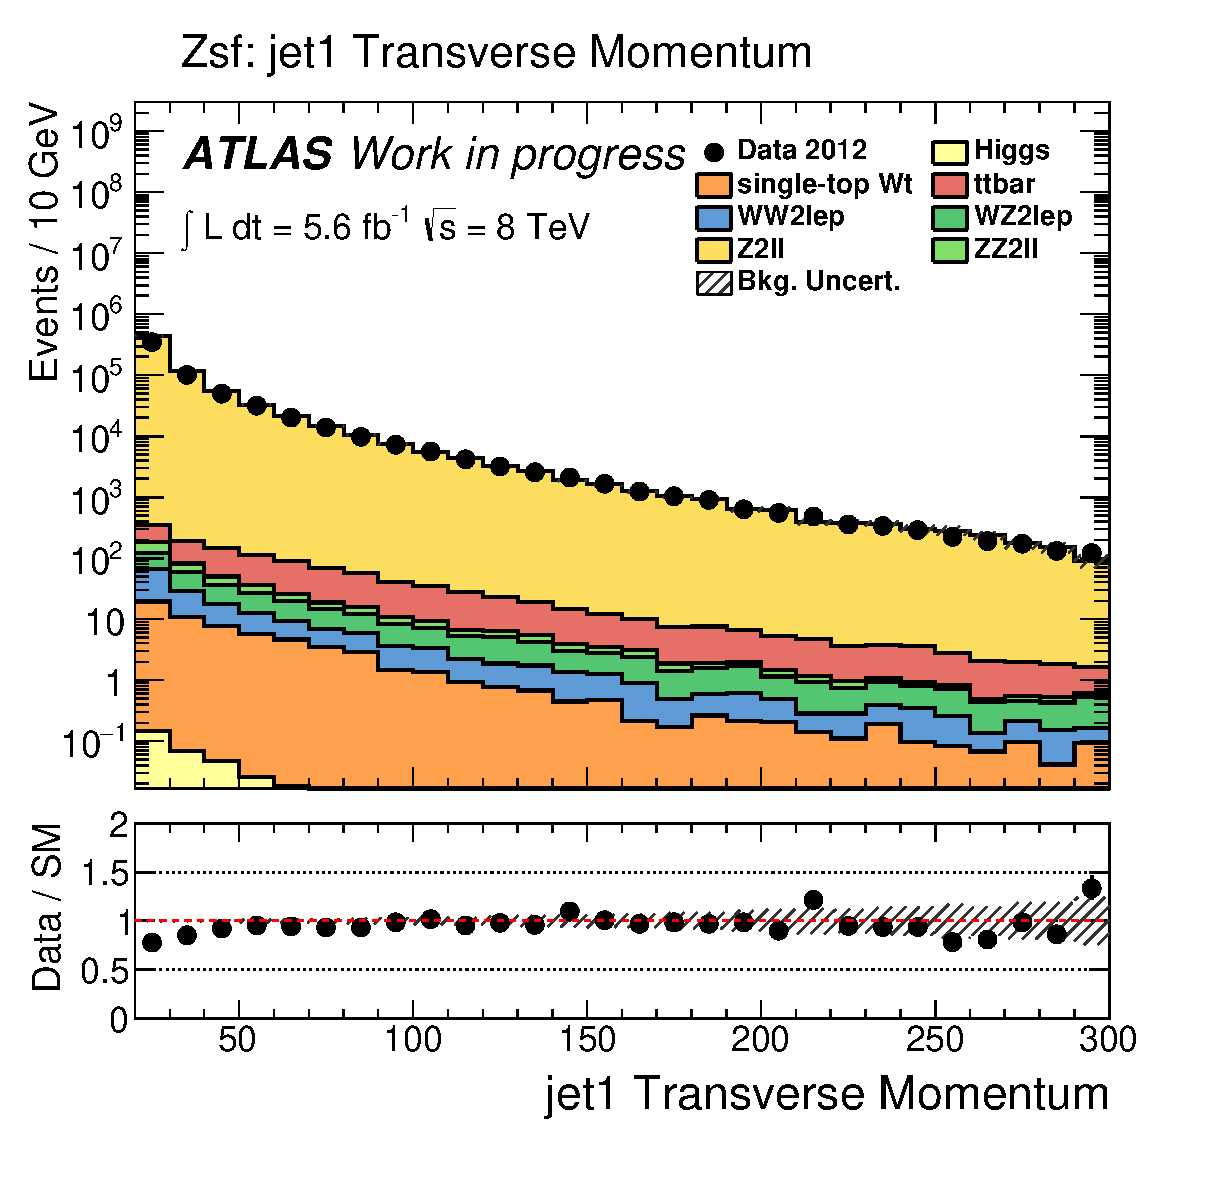
\includegraphics[width=0.8\textwidth]{../scp_landingpad/sf/Zsf_jet1Pt_iso}
			\column{0.4\paperwidth}
				\centering
				%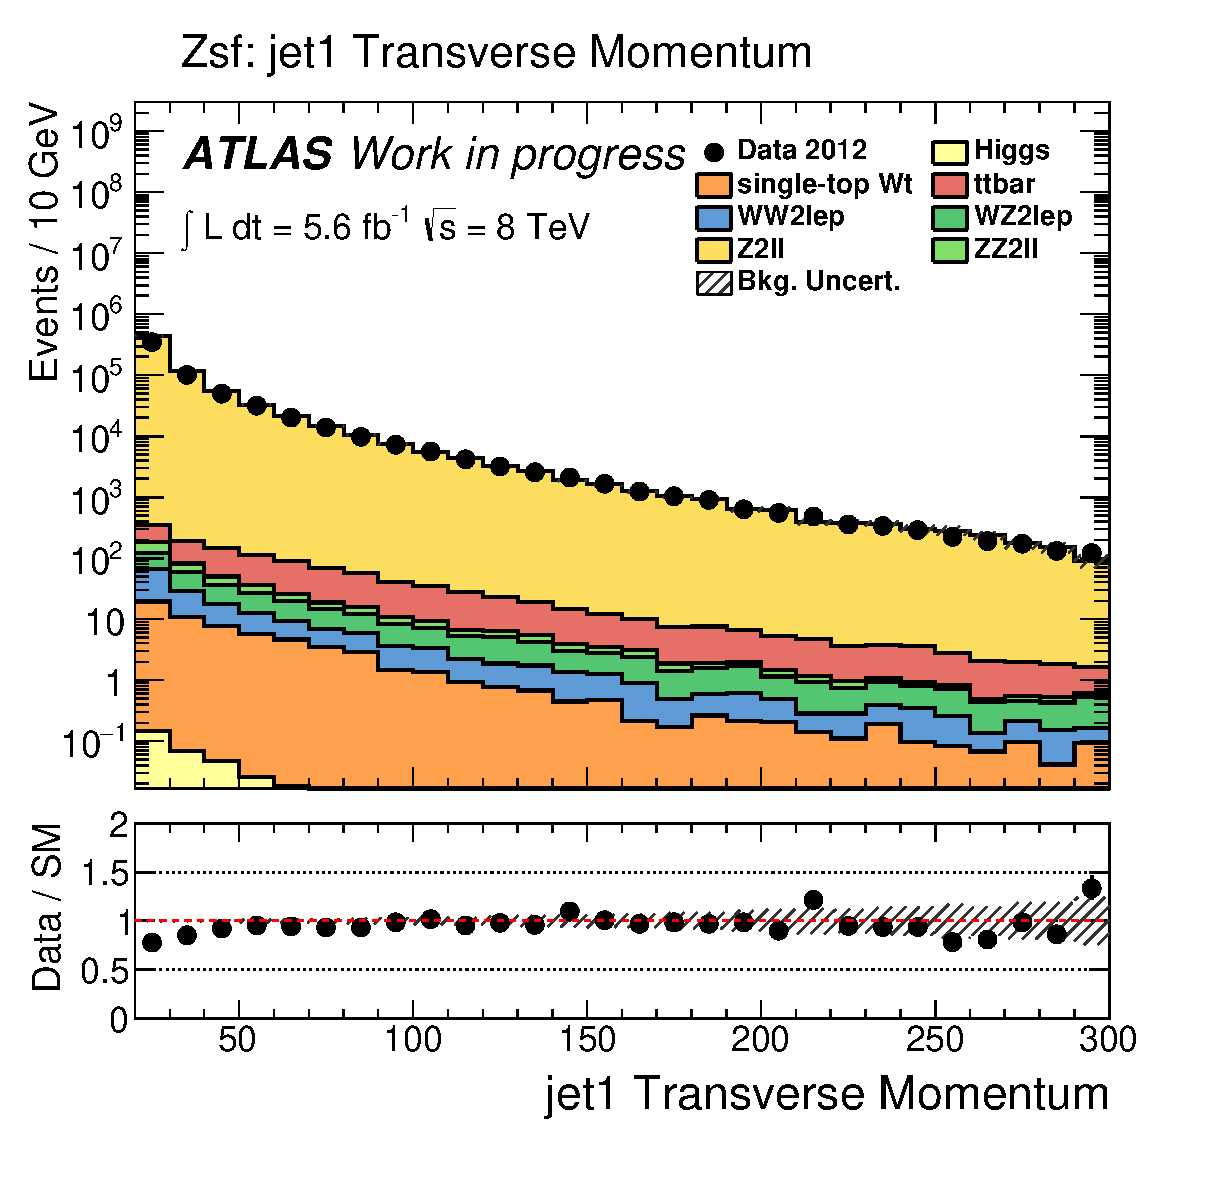
\includegraphics[height=4cm]{../scp_landingpad/sf/Zsf_jet1Pt_iso}
				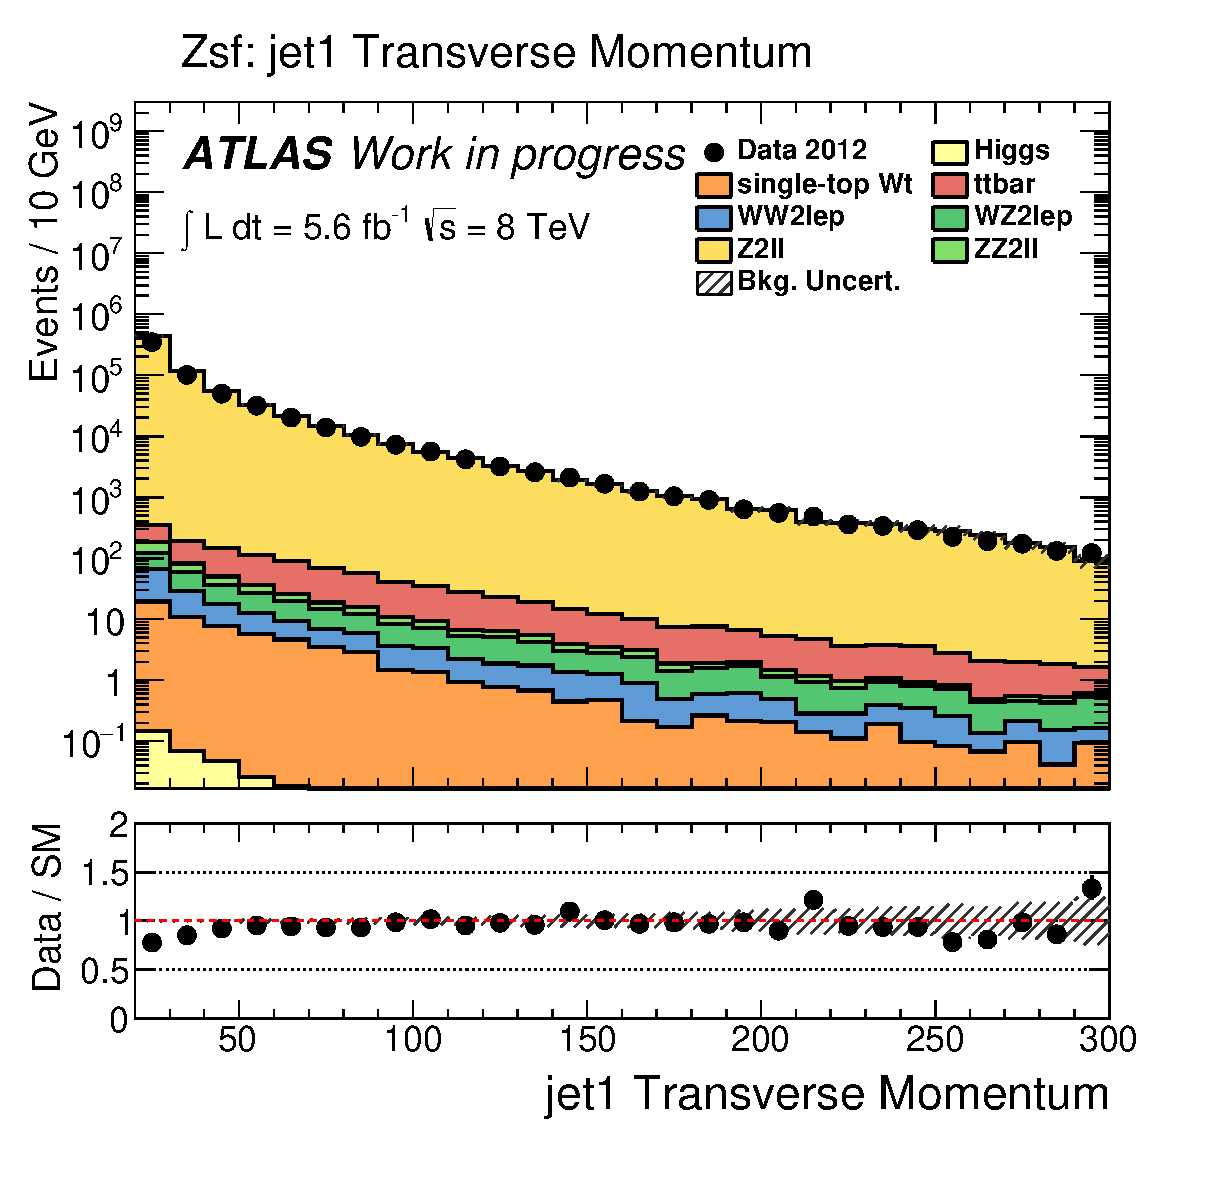
\includegraphics[width=0.8\textwidth]{../scp_landingpad/sf/Zsf_jet1Pt_iso}
			%	\centering
				%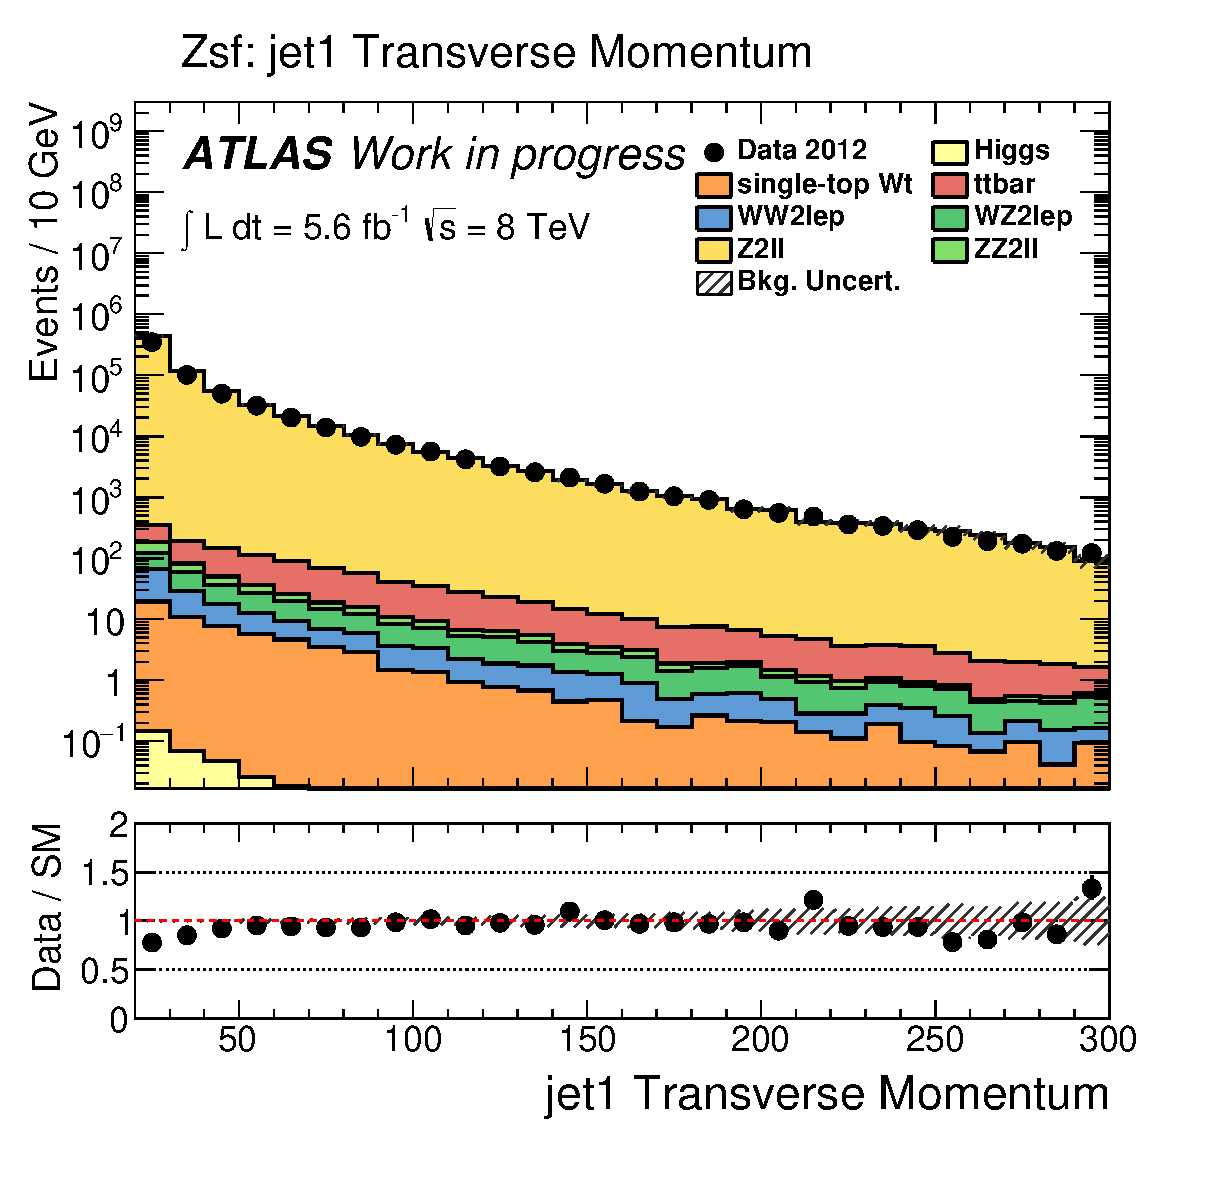
\includegraphics[width=1.2\textwidth]{../scp_landingpad/sf/Zsf_jet1Pt_iso}
		%	\end{column}
%			\begin{column}[T]{3cm}
%				\centering
%				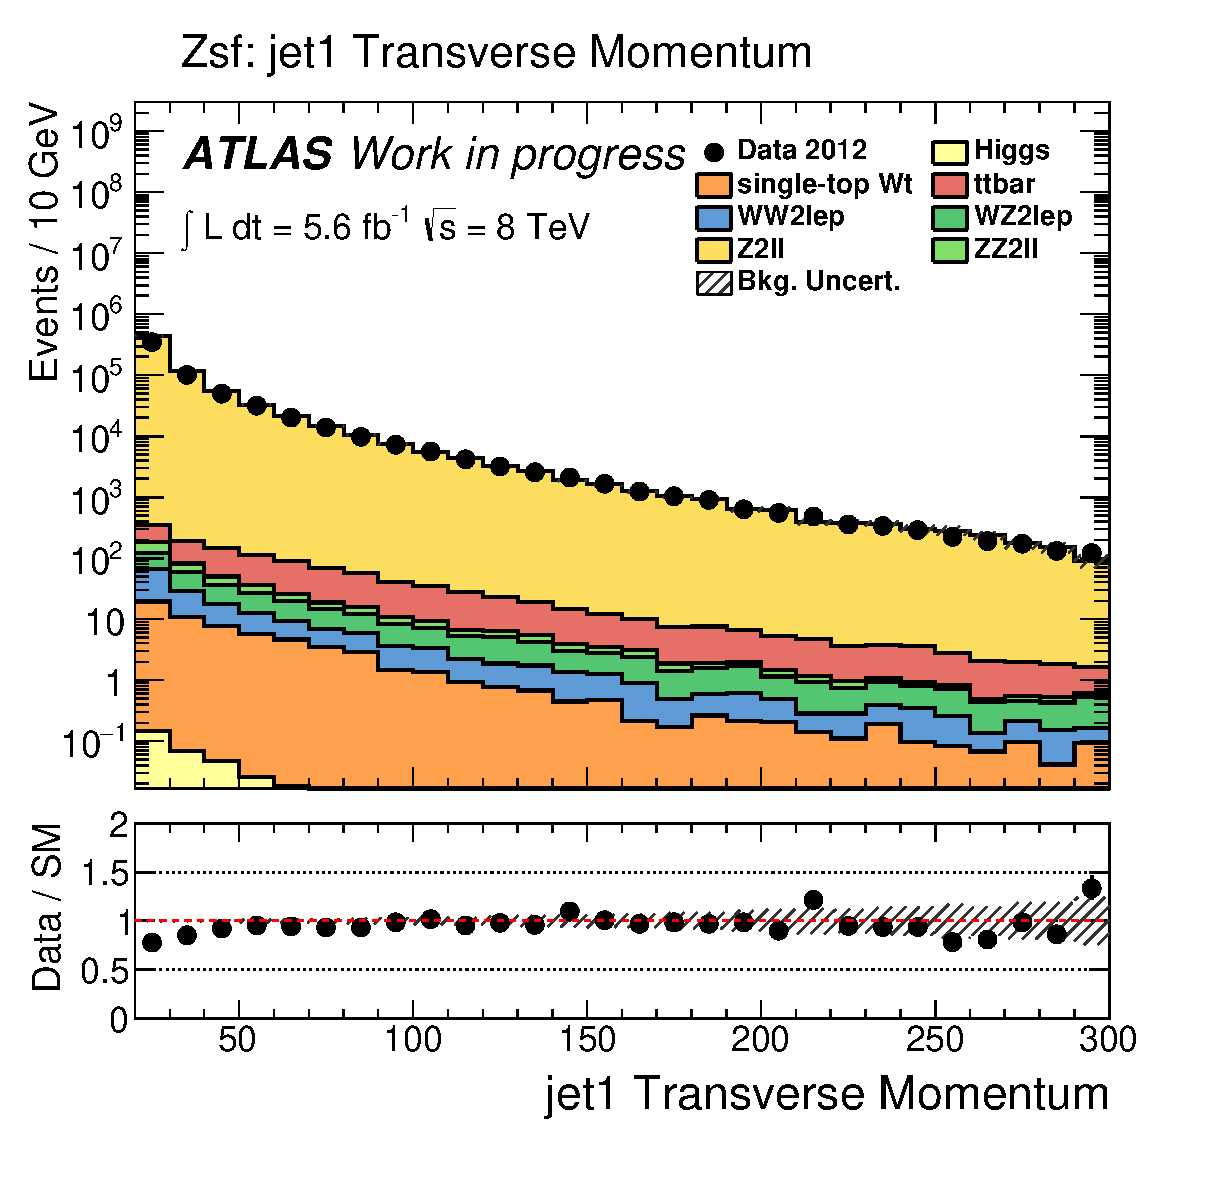
\includegraphics[height=3cm]{../scp_landingpad/sf/Zsf_jet1Pt_iso}
%			%					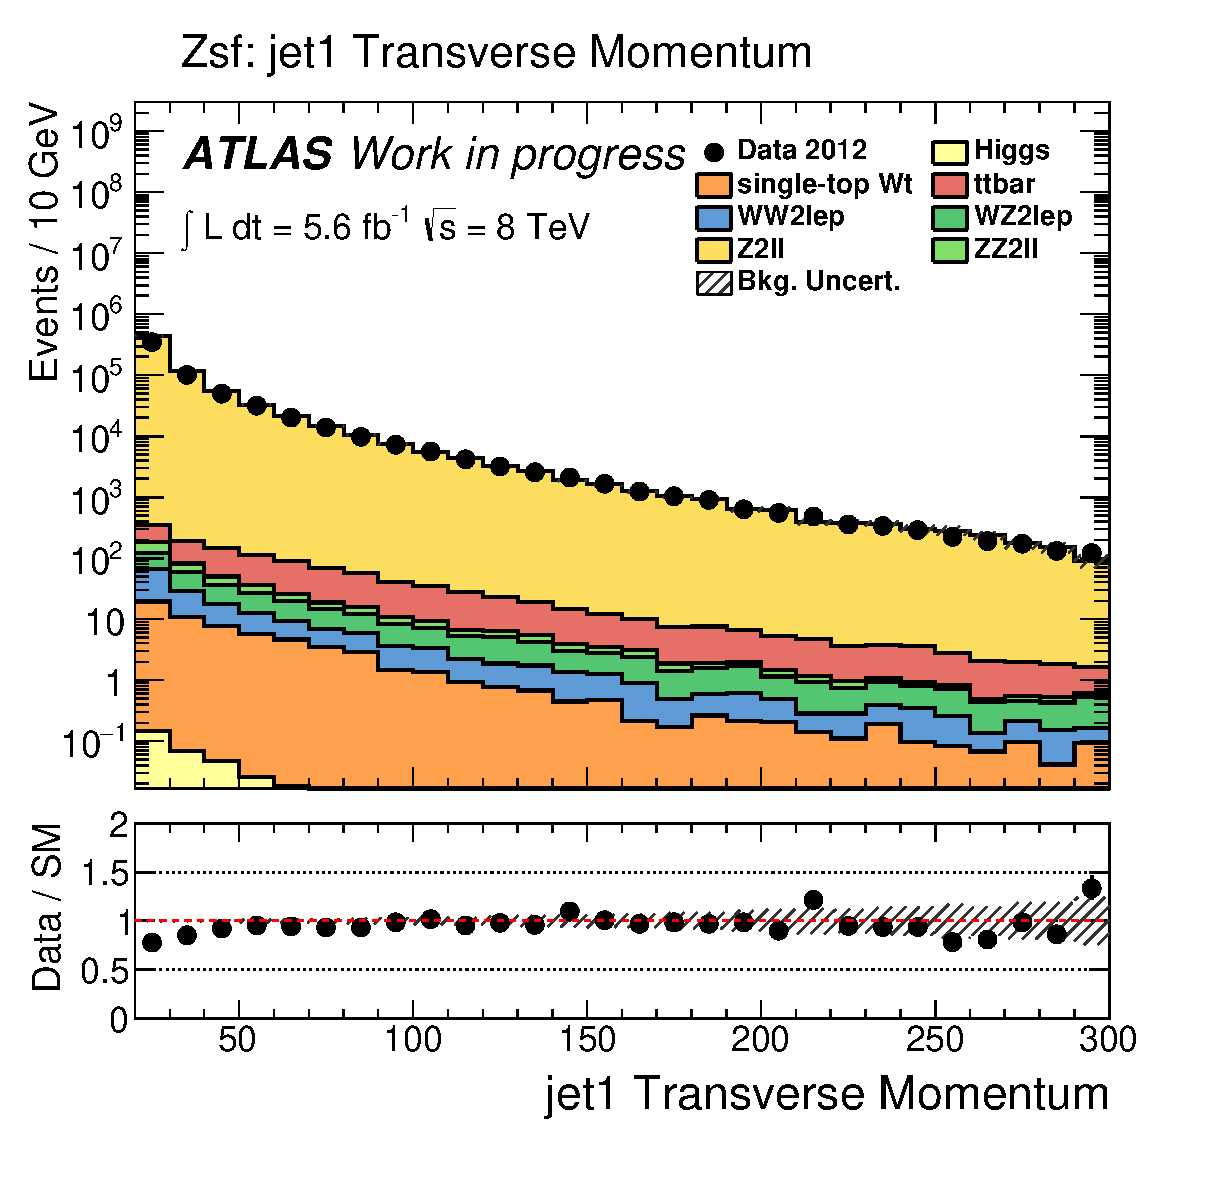
\includegraphics[width=1.2\textwidth]{../scp_landingpad/sf/Zsf_jet1Pt_iso}
%			\end{column}
%			\begin{column}[T]{3cm}
%				\centering
%				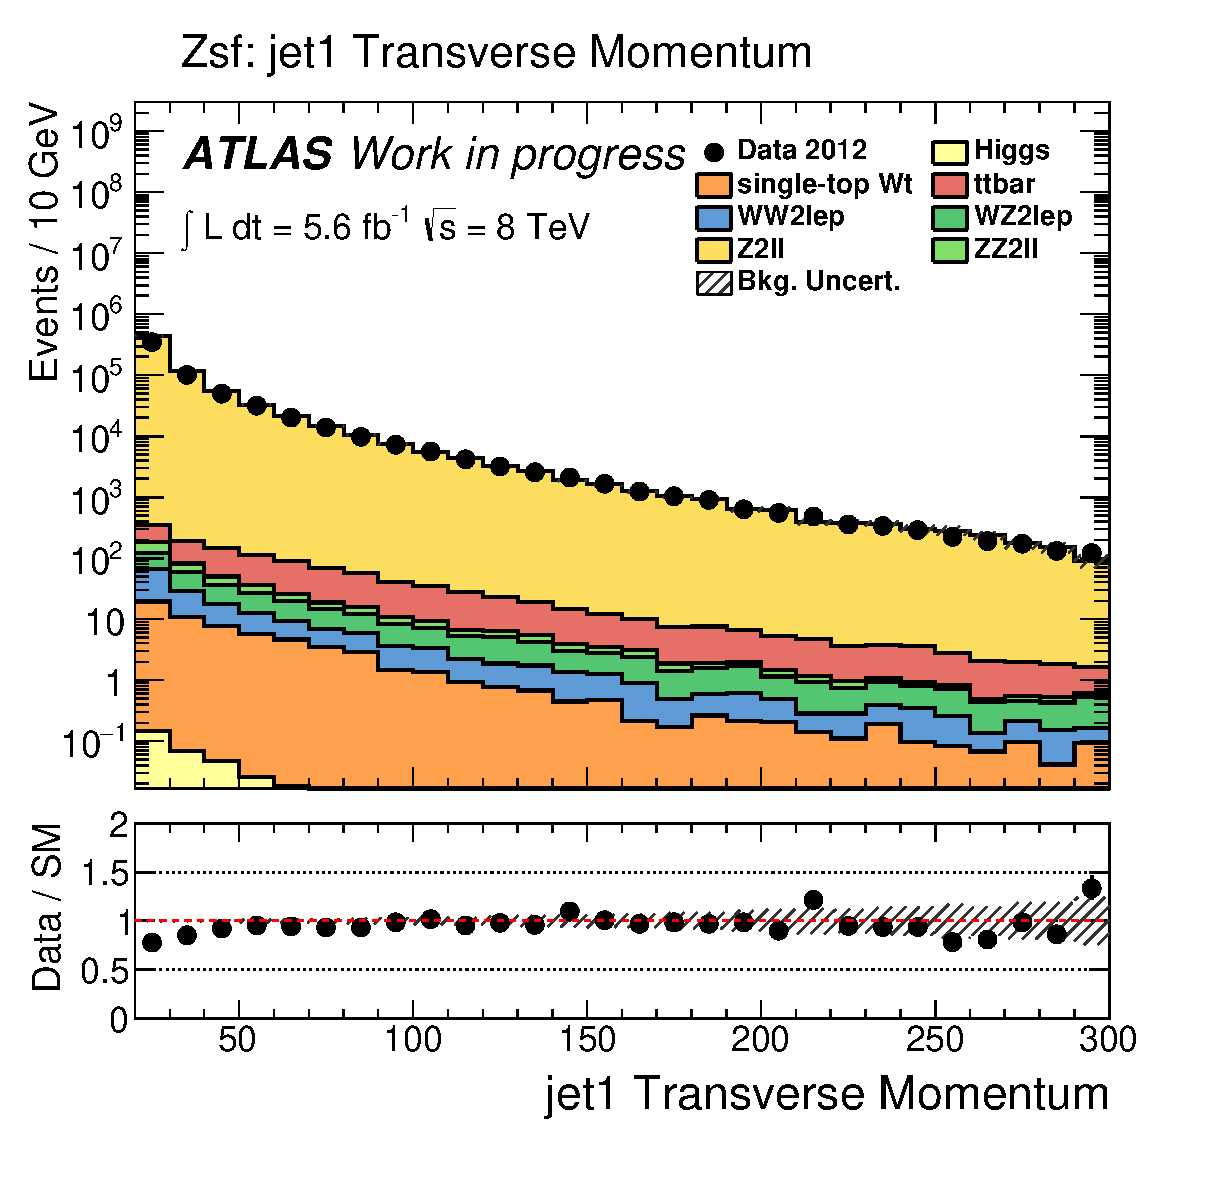
\includegraphics[height=3cm]{../scp_landingpad/sf/Zsf_jet1Pt_iso}
%			%					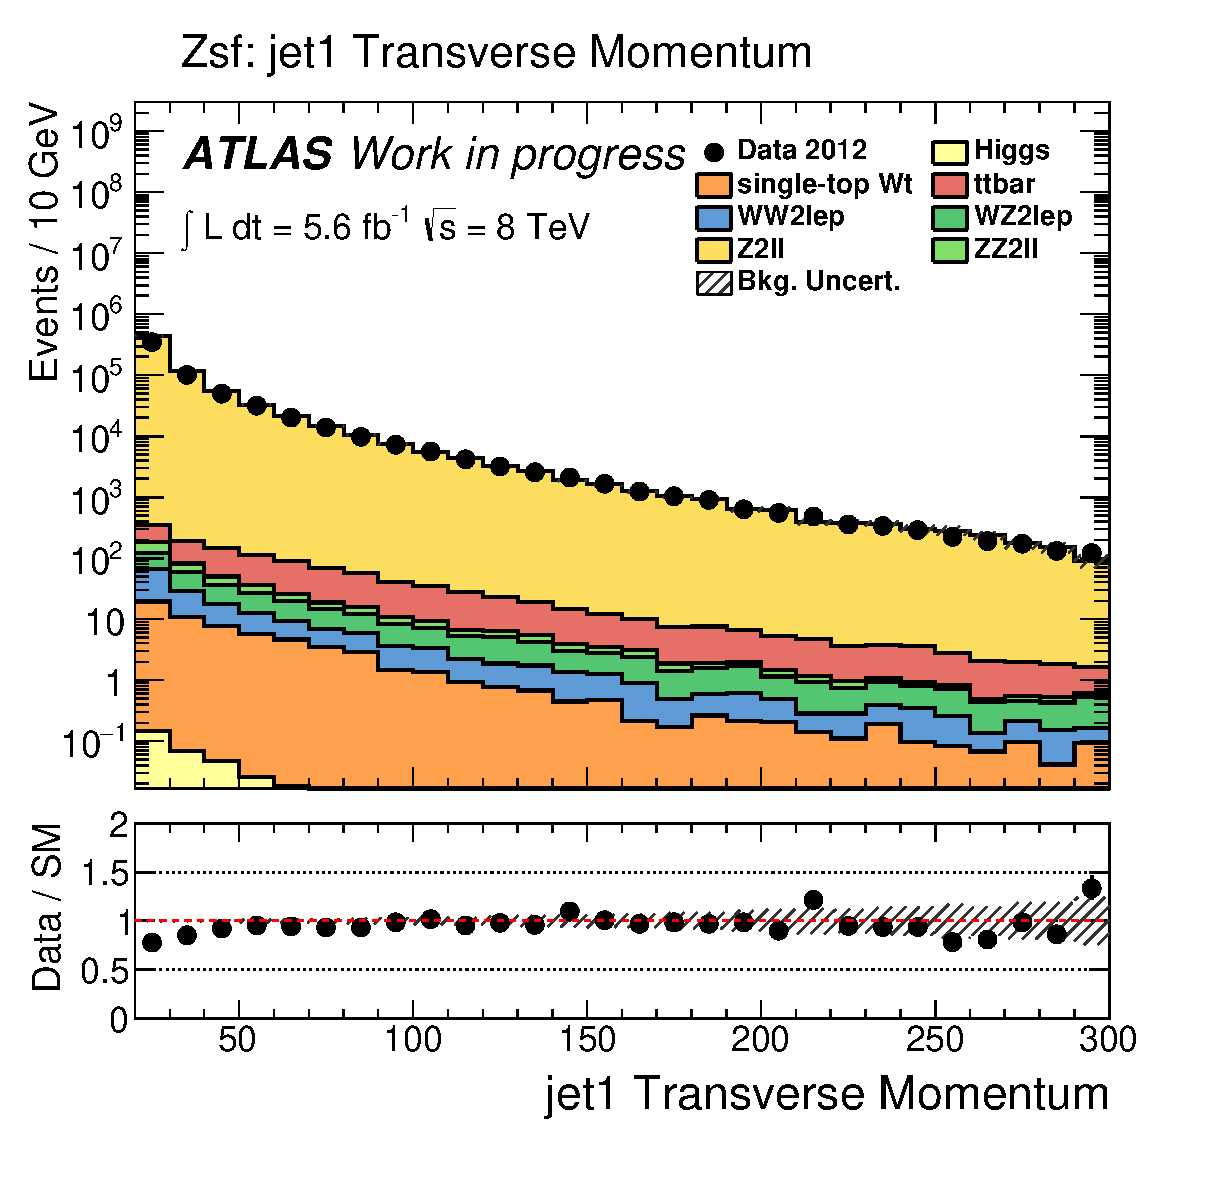
\includegraphics[width=1.2\textwidth]{../scp_landingpad/sf/Zsf_jet1Pt_iso}
%			\end{column}
		\end{columns}


	\end{block}

	\begin{block}{}  % for upper row of figures
		\begin{columns}[c]
		%	\centering
			\column{0.4\paperwidth}
				\centering
				%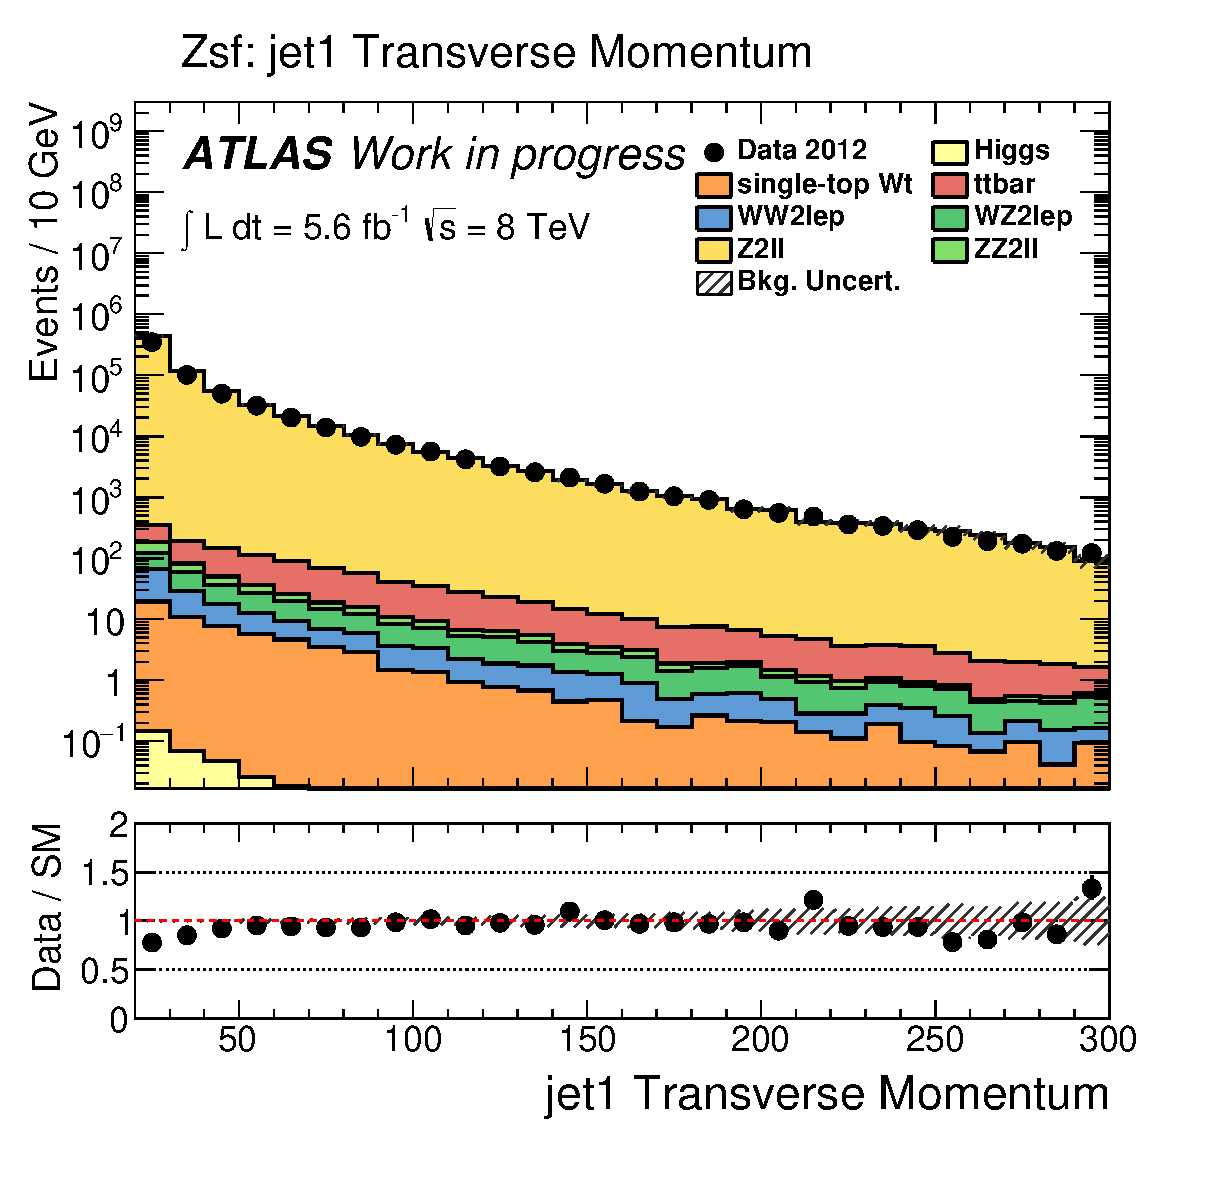
\includegraphics[height=4cm]{../scp_landingpad/sf/Zsf_jet1Pt_iso}
				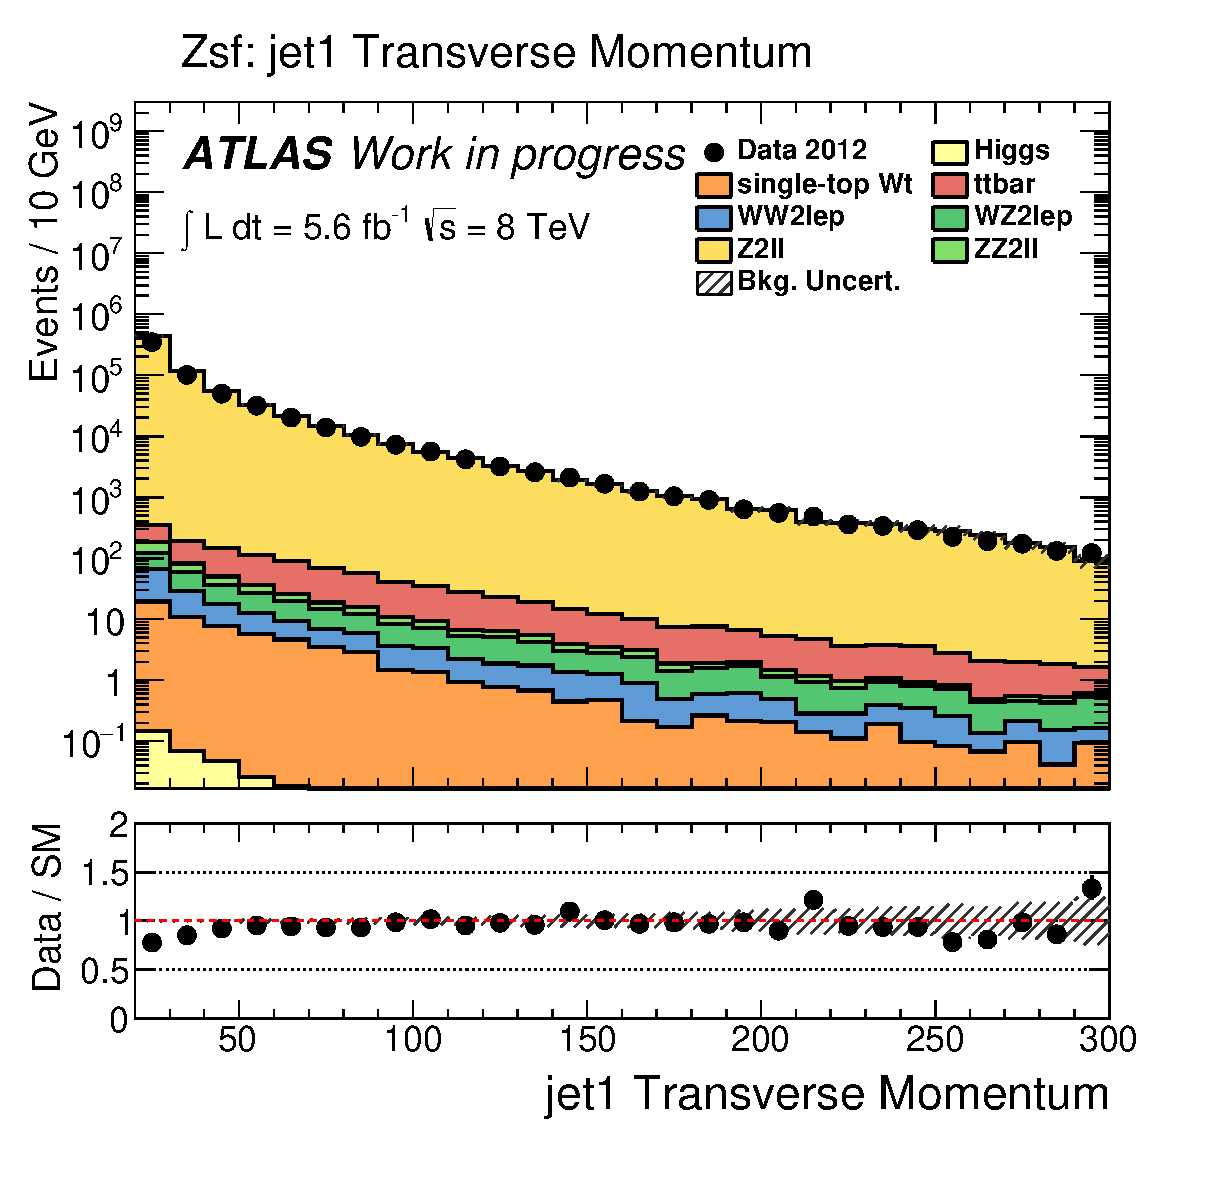
\includegraphics[width=0.8\textwidth]{../scp_landingpad/sf/Zsf_jet1Pt_iso}
			\column{0.4\paperwidth}
				\centering
				%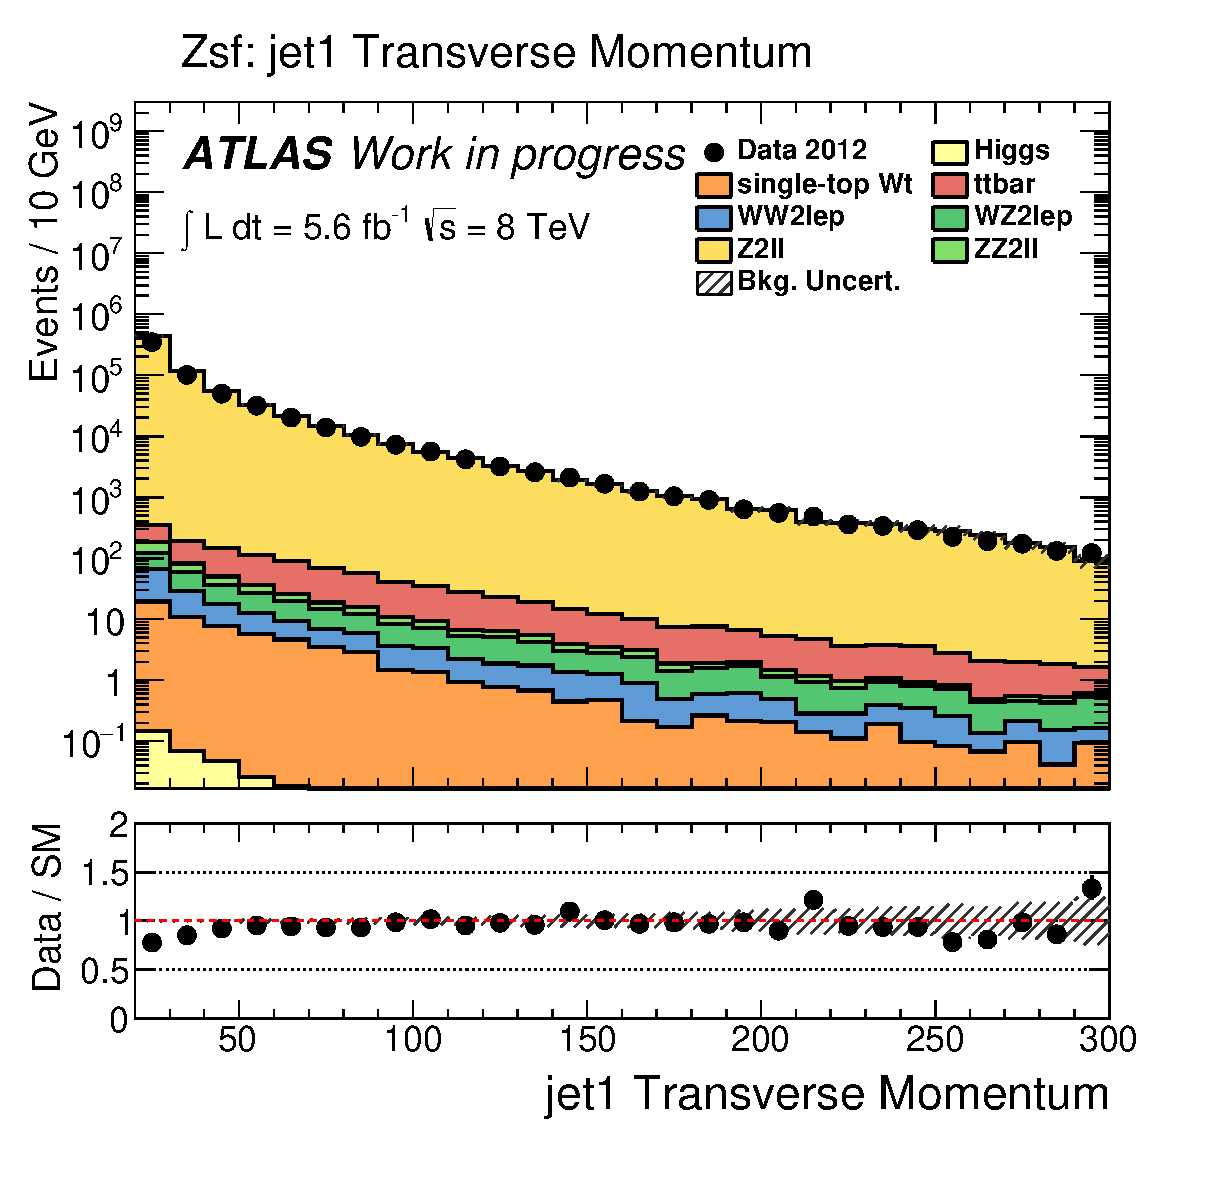
\includegraphics[height=4cm]{../scp_landingpad/sf/Zsf_jet1Pt_iso}
				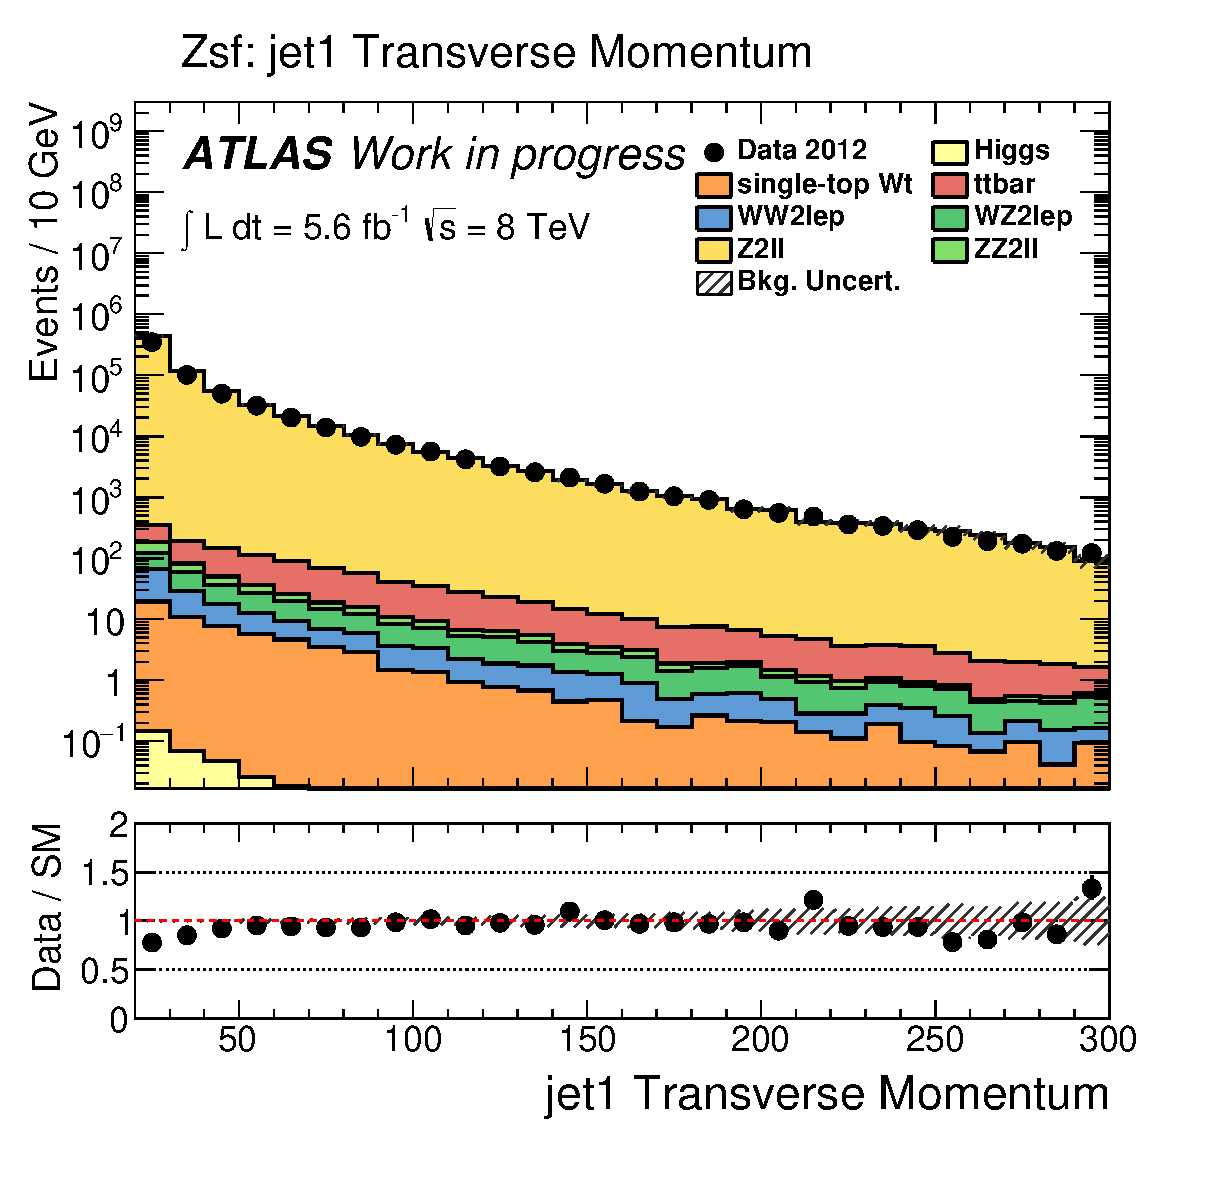
\includegraphics[width=0.8\textwidth]{../scp_landingpad/sf/Zsf_jet1Pt_iso}
			%	\centering
				%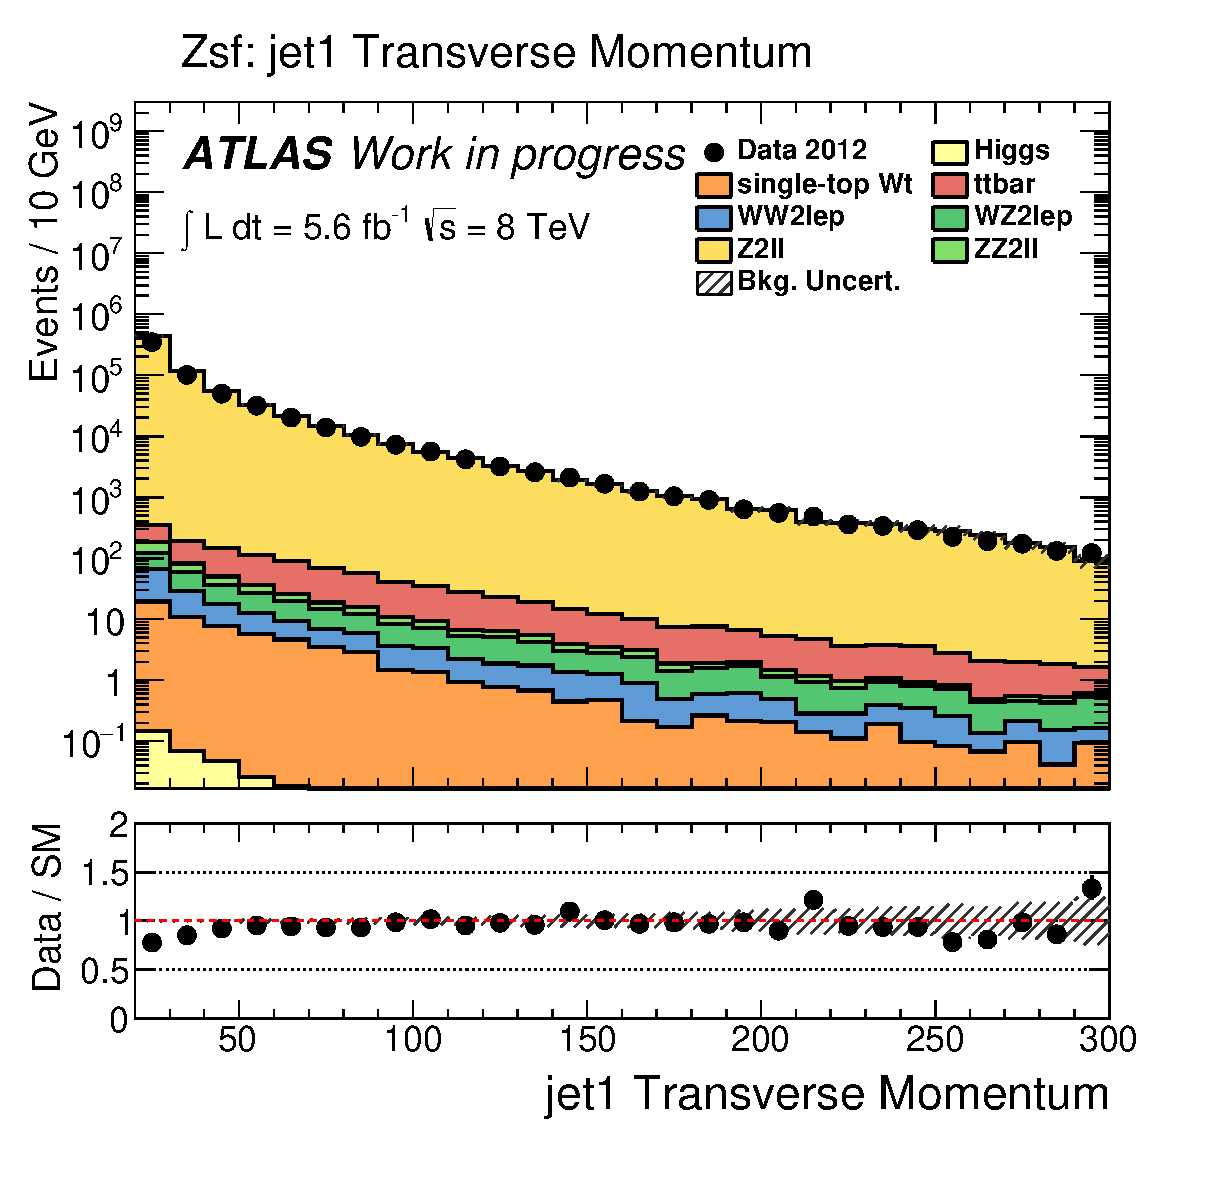
\includegraphics[width=1.2\textwidth]{../scp_landingpad/sf/Zsf_jet1Pt_iso}
		%	\end{column}
%			\begin{column}[T]{3cm}
%				\centering
%				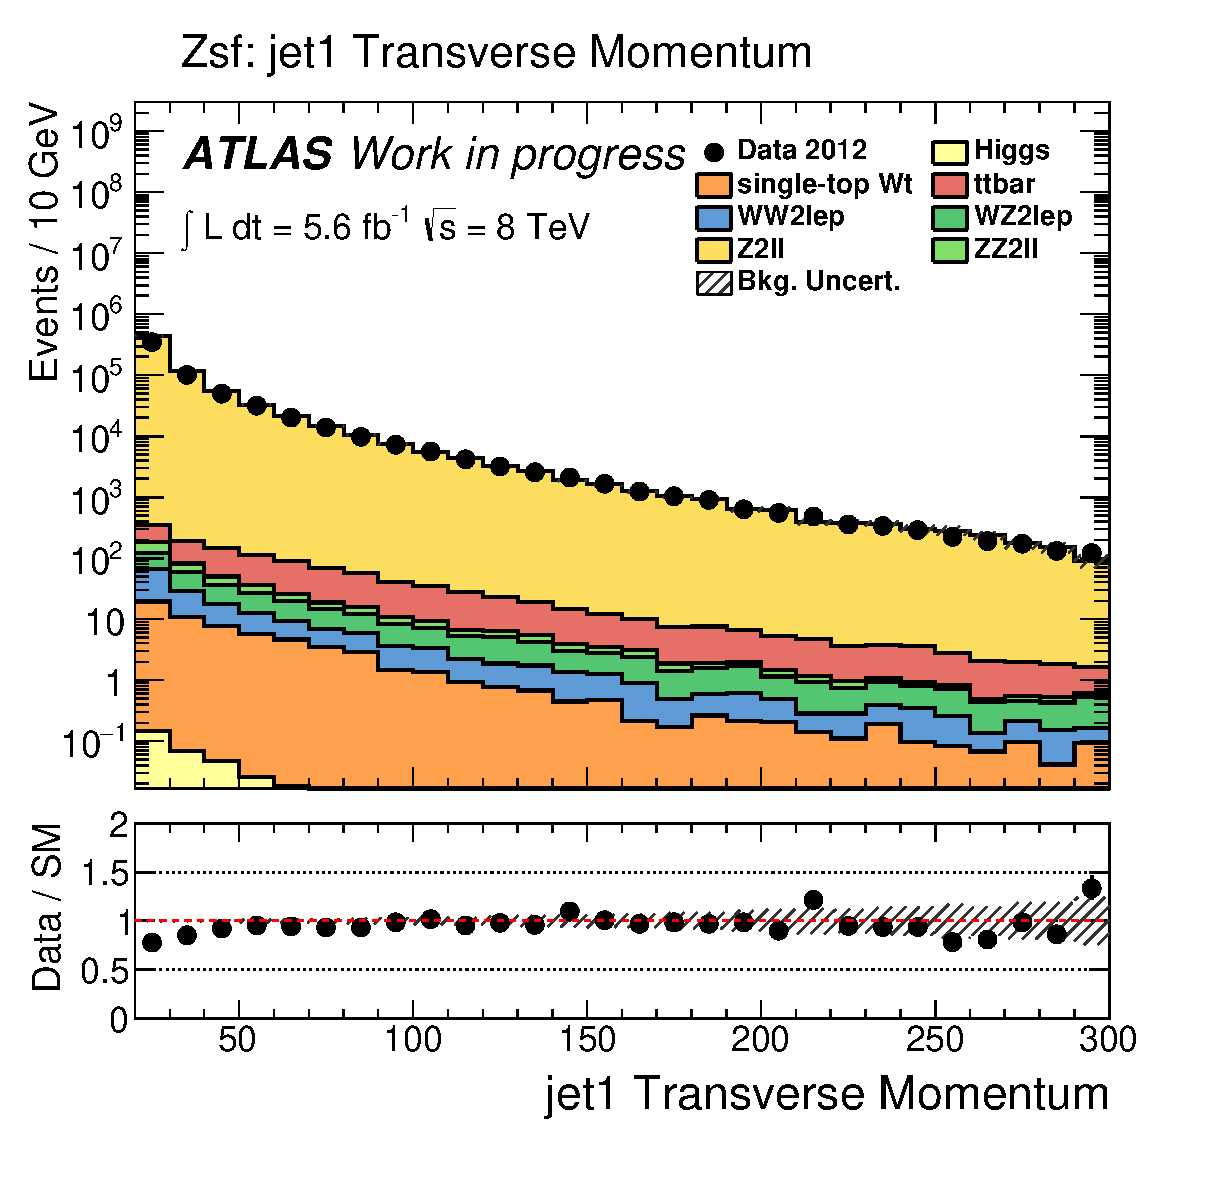
\includegraphics[height=3cm]{../scp_landingpad/sf/Zsf_jet1Pt_iso}
%			%					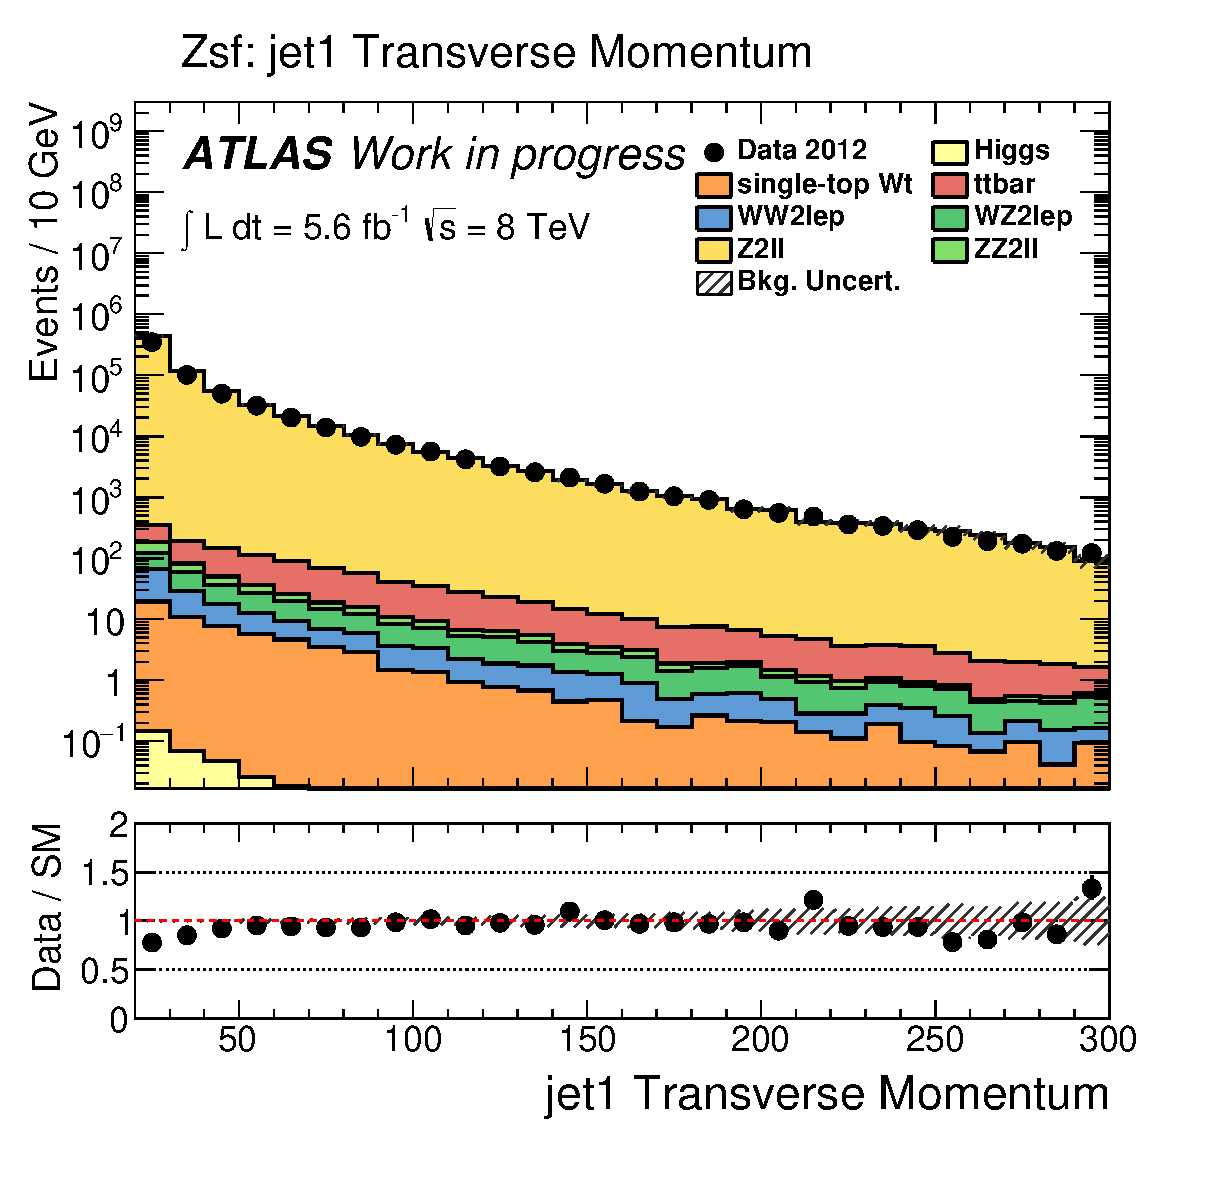
\includegraphics[width=1.2\textwidth]{../scp_landingpad/sf/Zsf_jet1Pt_iso}
%			\end{column}
%			\begin{column}[T]{3cm}
%				\centering
%				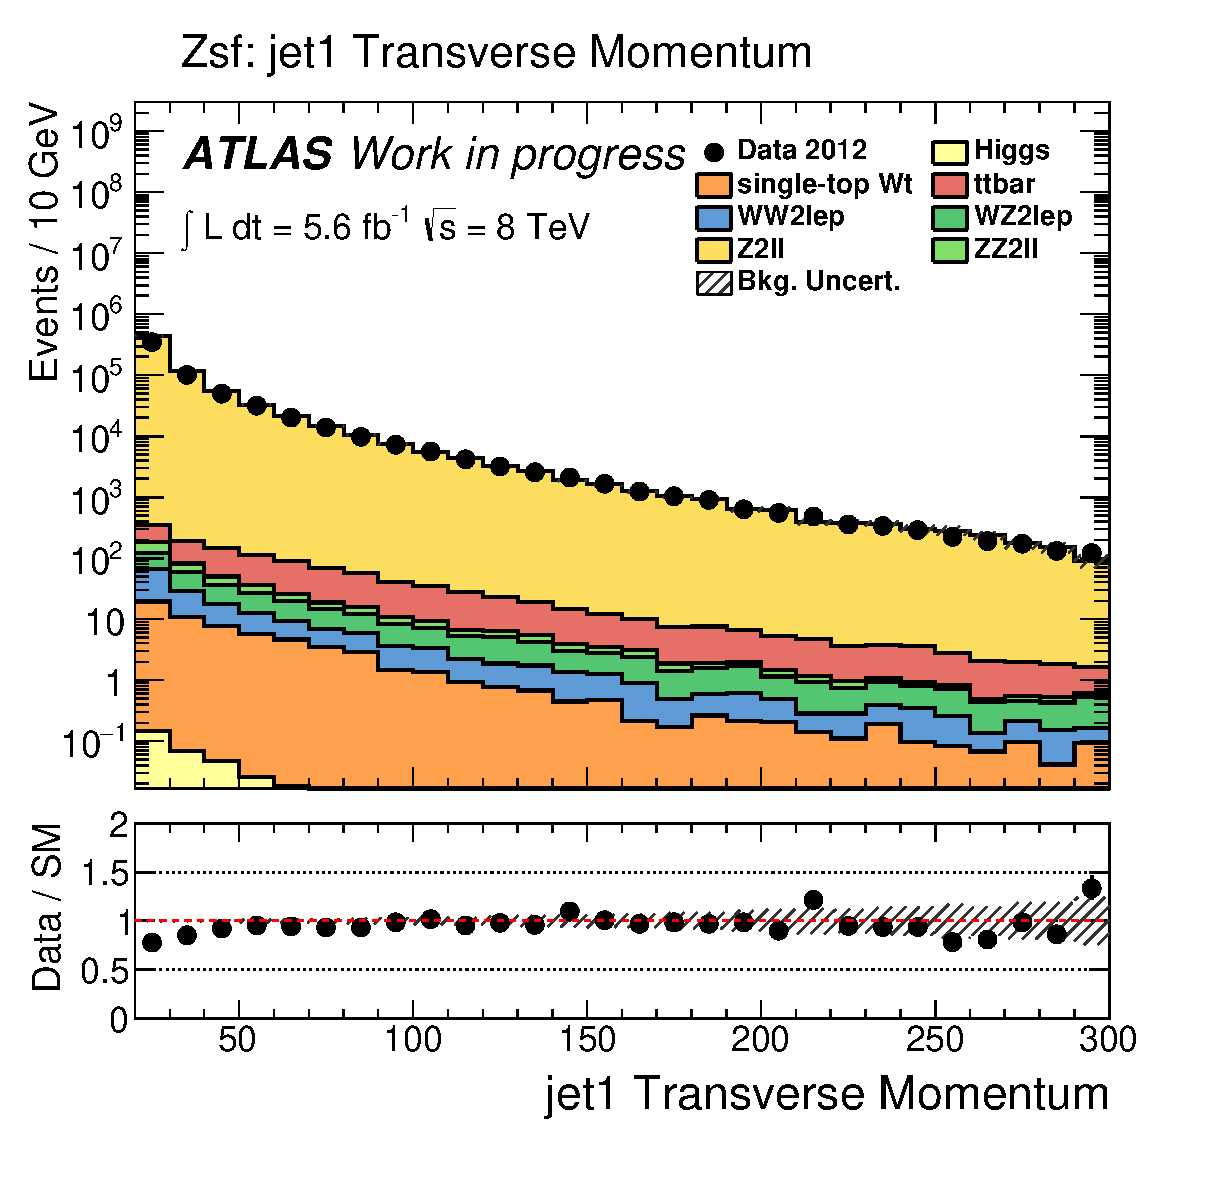
\includegraphics[height=3cm]{../scp_landingpad/sf/Zsf_jet1Pt_iso}
%			%					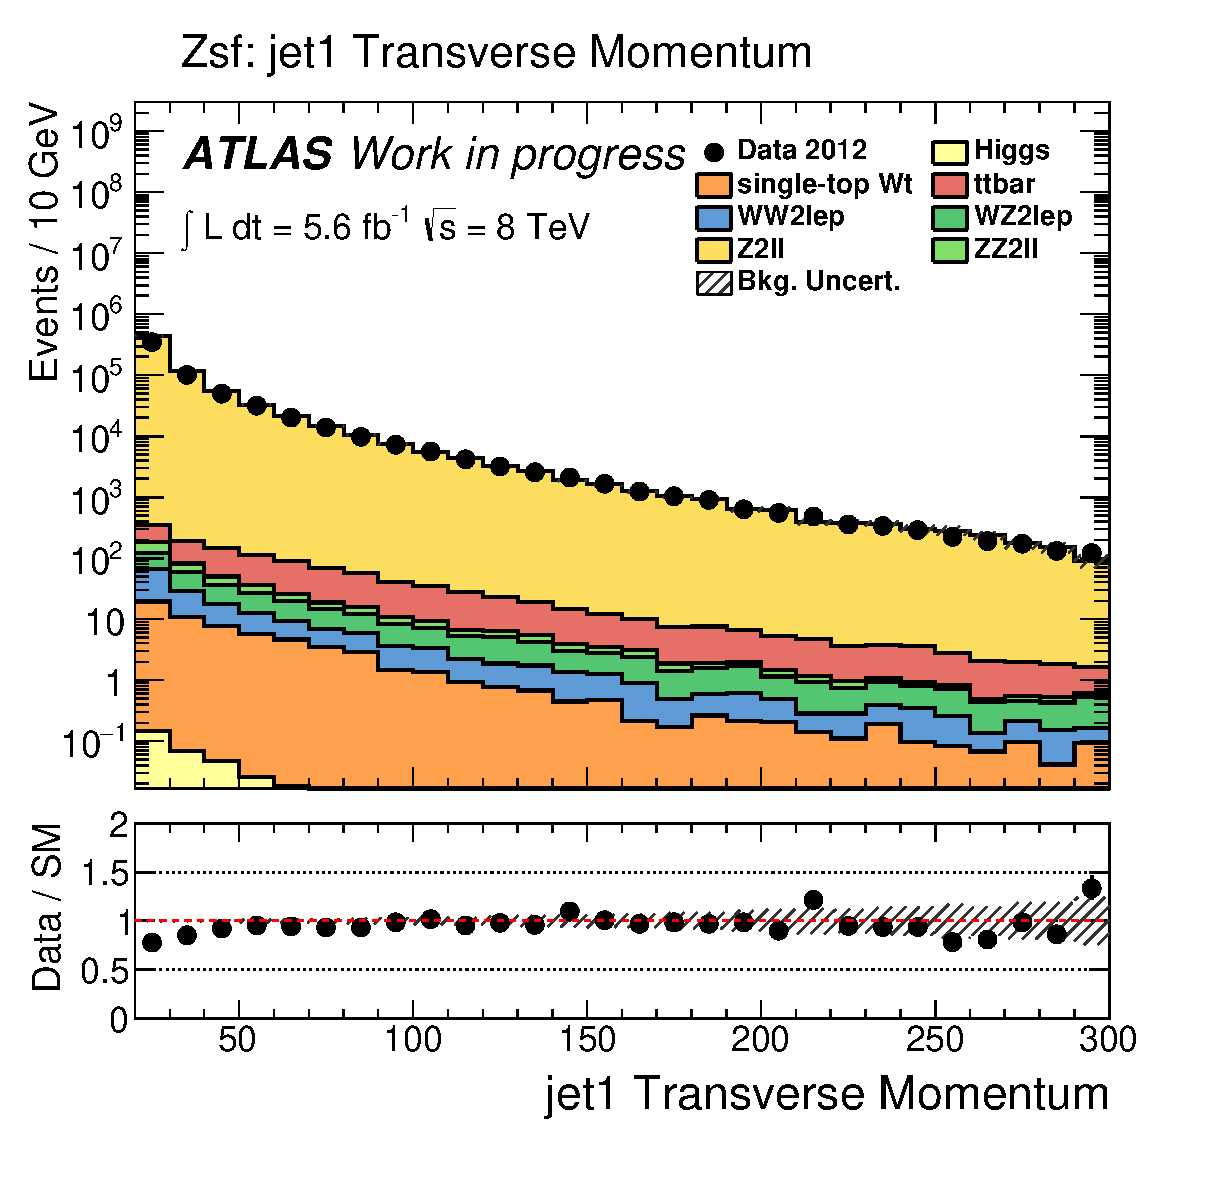
\includegraphics[width=1.2\textwidth]{../scp_landingpad/sf/Zsf_jet1Pt_iso}
%			\end{column}
		\end{columns}


	\end{block}

		\end{frame}
\begin{frame}{Example of columns -- 6 fig}

	\begin{block}{}  % for upper row of figures
		\begin{columns}[c]
		%	\centering
			\column{0.33\paperwidth}
				\centering
				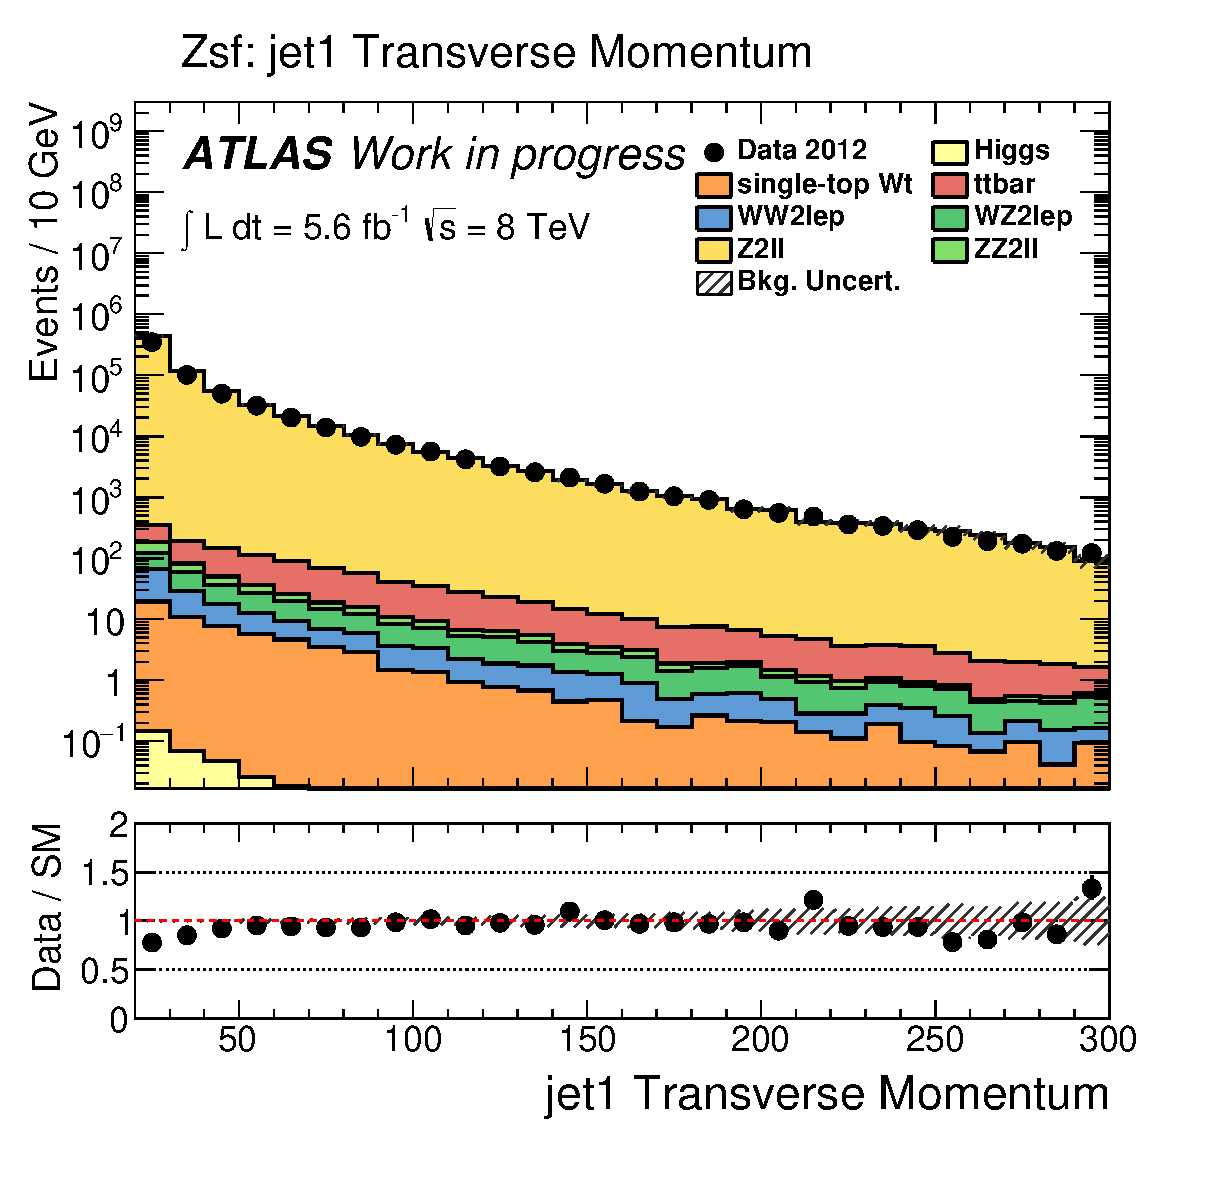
\includegraphics[width=0.95\textwidth]{../scp_landingpad/sf/Zsf_jet1Pt_iso}
			\column{0.33\paperwidth}
				\centering
				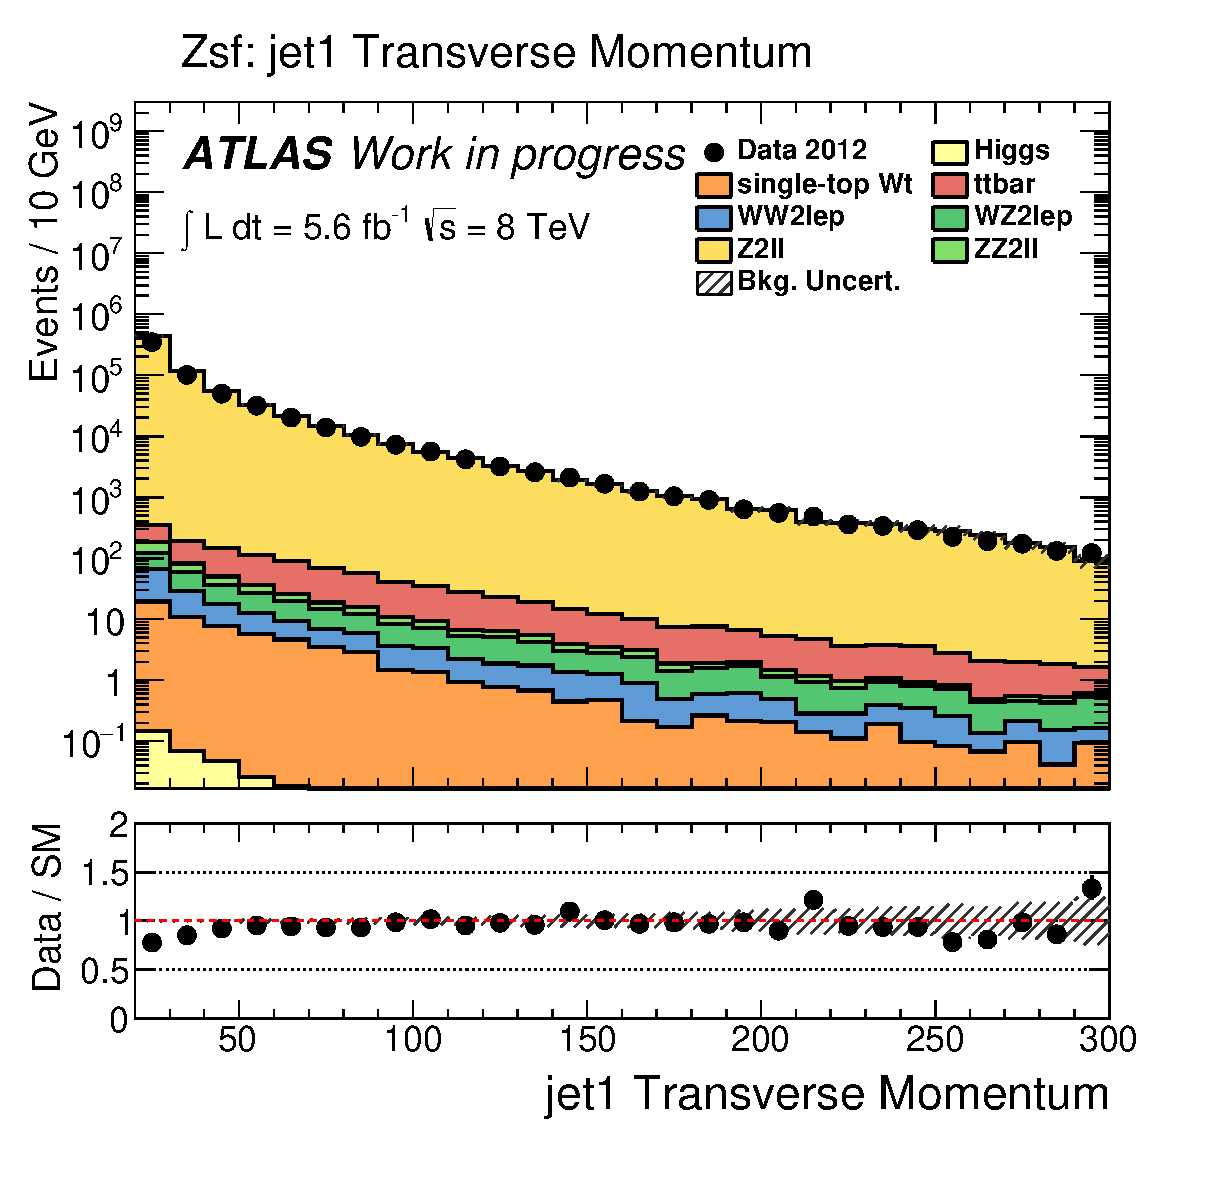
\includegraphics[width=0.95\textwidth]{../scp_landingpad/sf/Zsf_jet1Pt_iso}
			\column{0.33\paperwidth}
				\centering
				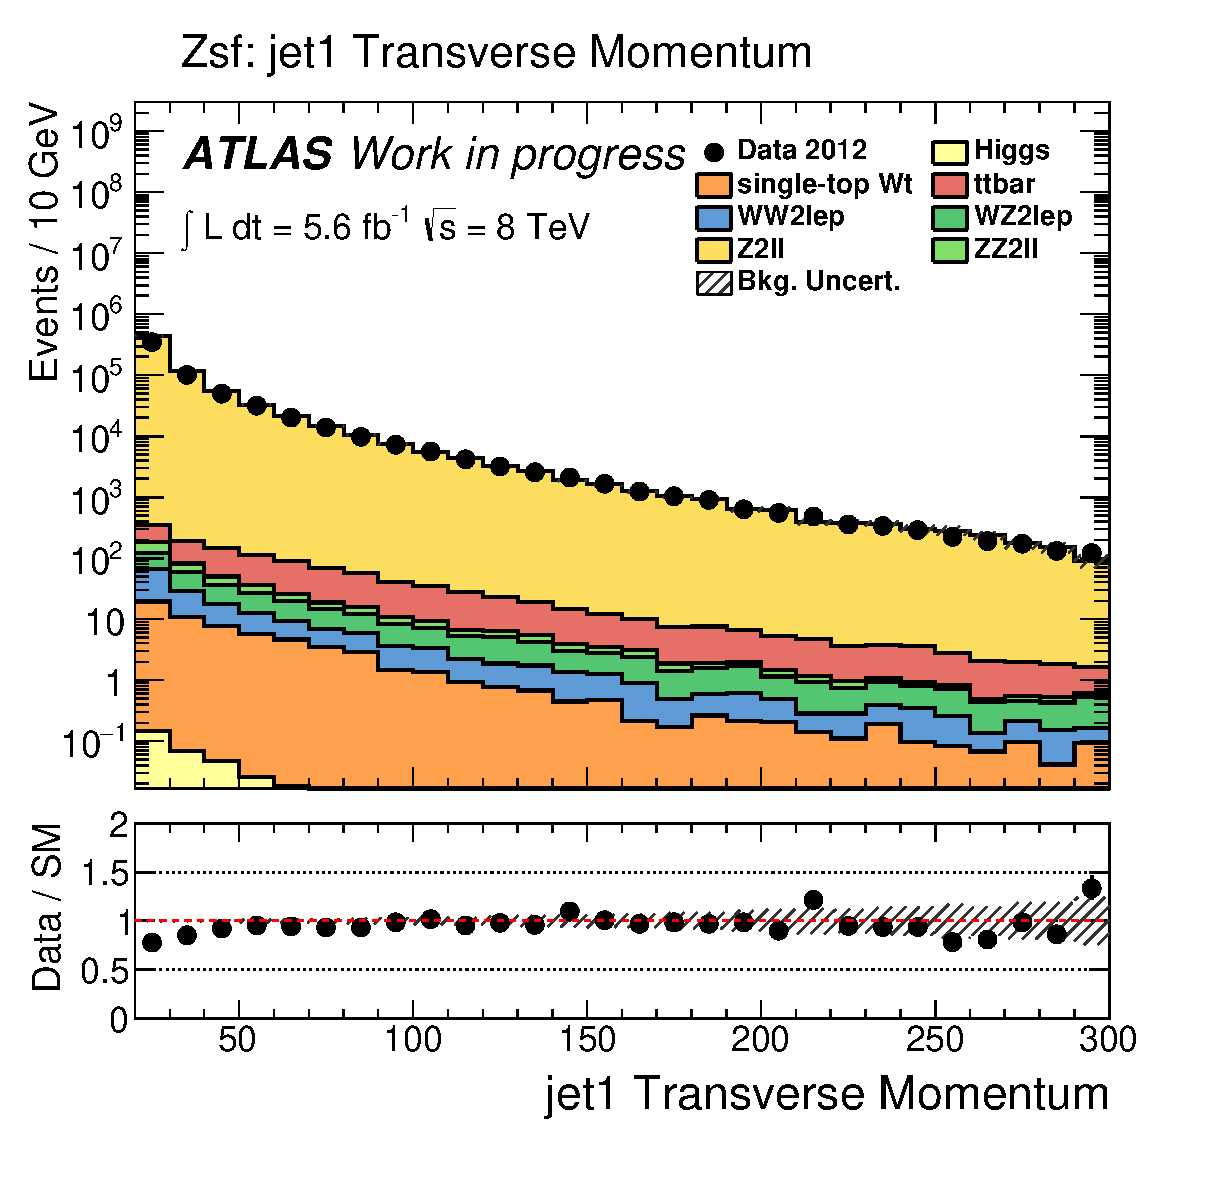
\includegraphics[width=0.95\textwidth]{../scp_landingpad/sf/Zsf_jet1Pt_iso}

		\end{columns}
	\end{block}
	\begin{block}{}  % for upper row of figures
		\begin{columns}[c]
		%	\centering
			\column{0.33\paperwidth}
				\centering
				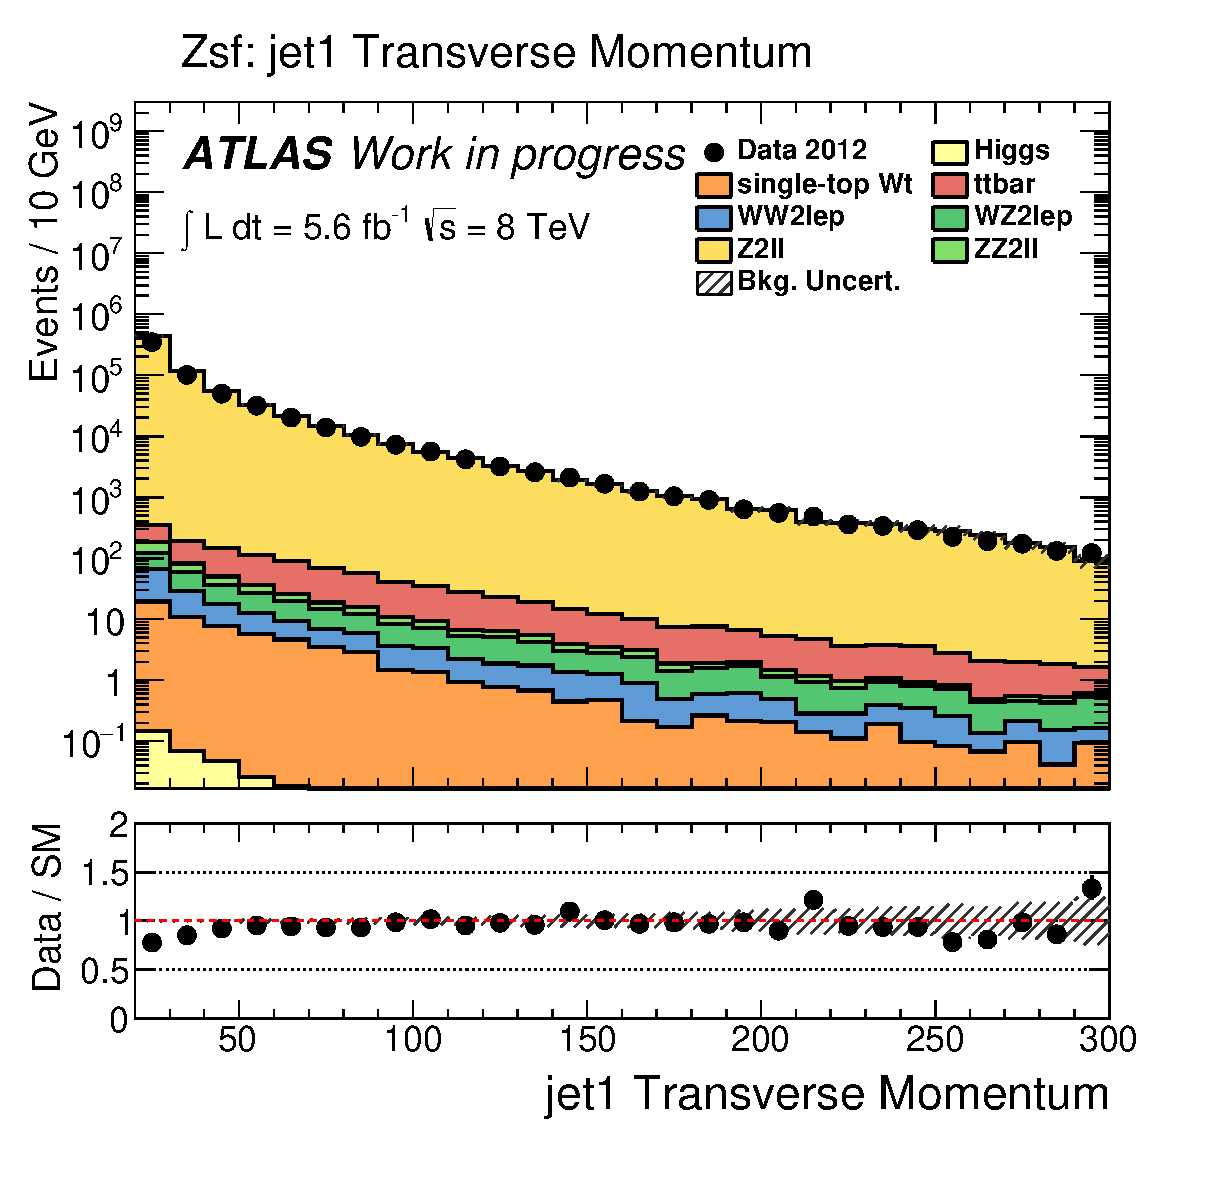
\includegraphics[width=0.95\textwidth]{../scp_landingpad/sf/Zsf_jet1Pt_iso}
			\column{0.33\paperwidth}
				\centering
				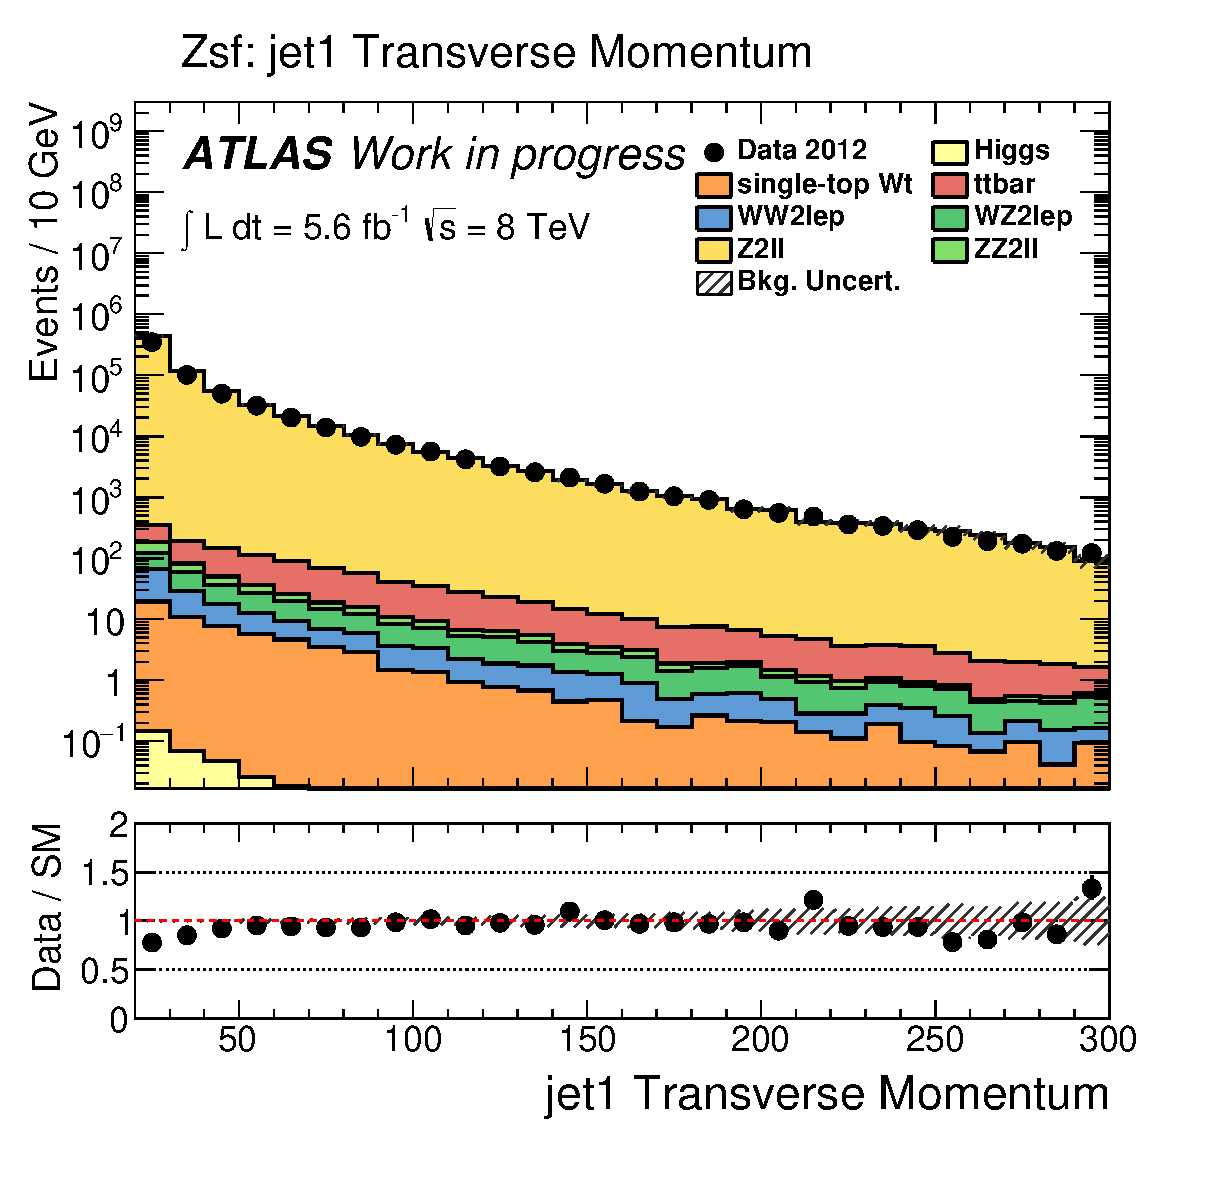
\includegraphics[width=0.95\textwidth]{../scp_landingpad/sf/Zsf_jet1Pt_iso}
			\column{0.33\paperwidth}
				\centering
				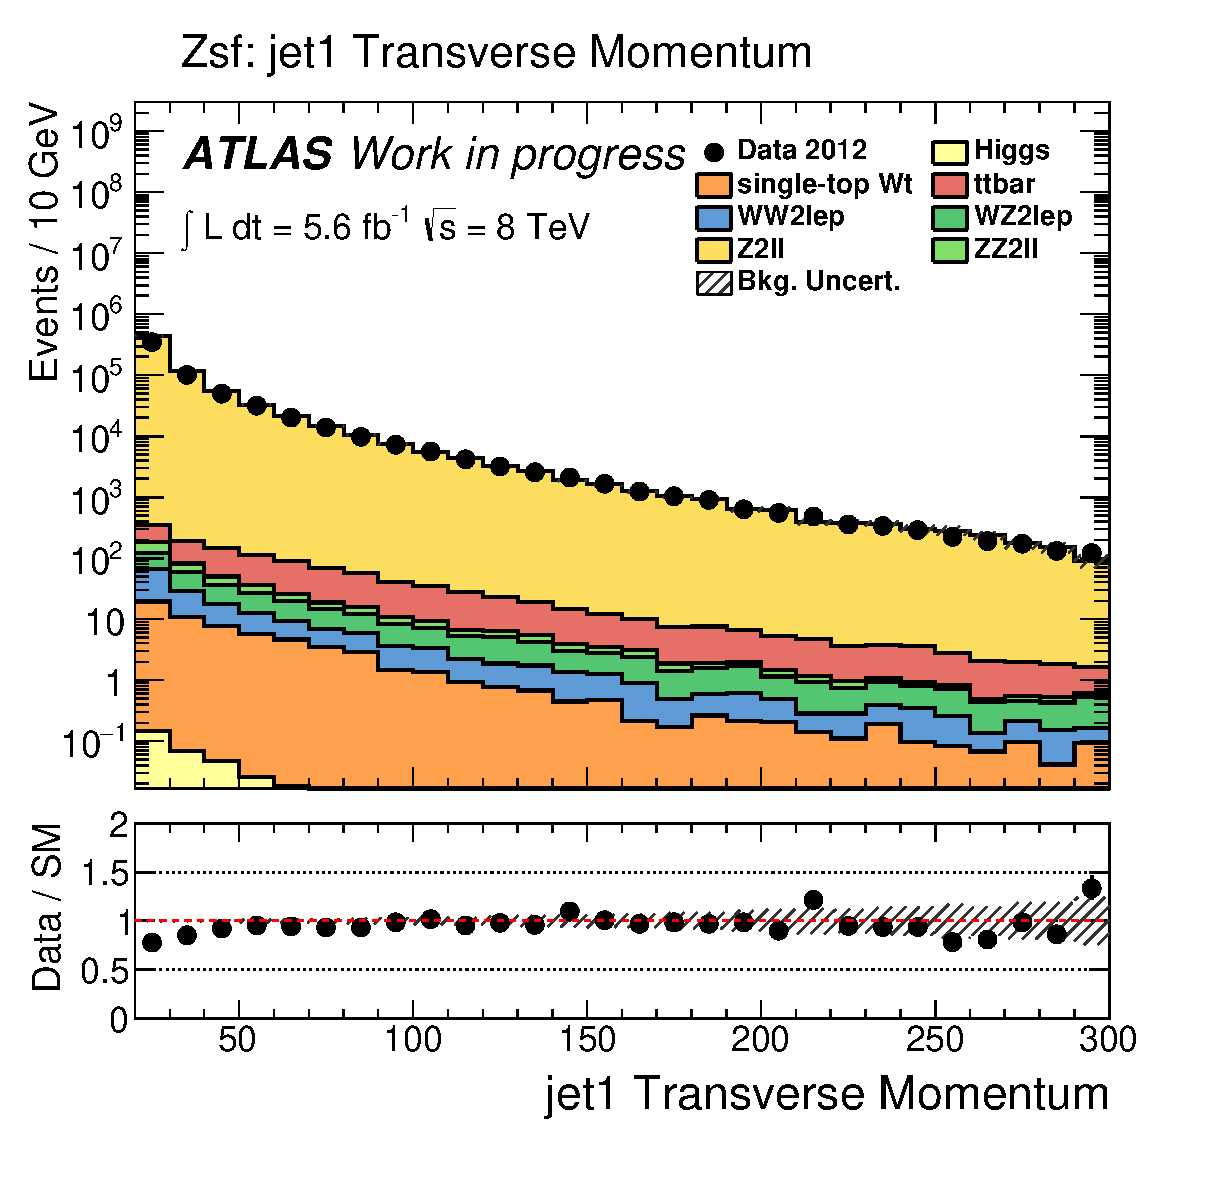
\includegraphics[width=0.95\textwidth]{../scp_landingpad/sf/Zsf_jet1Pt_iso}

		\end{columns}


	\end{block}
\end{frame}


\begin{frame}{Example of columns -- 4 wide}

	\begin{block}{}  % for upper row of figures
		\begin{columns}[c]
		%	\centering
			\column{0.25\paperwidth}
				\centering
				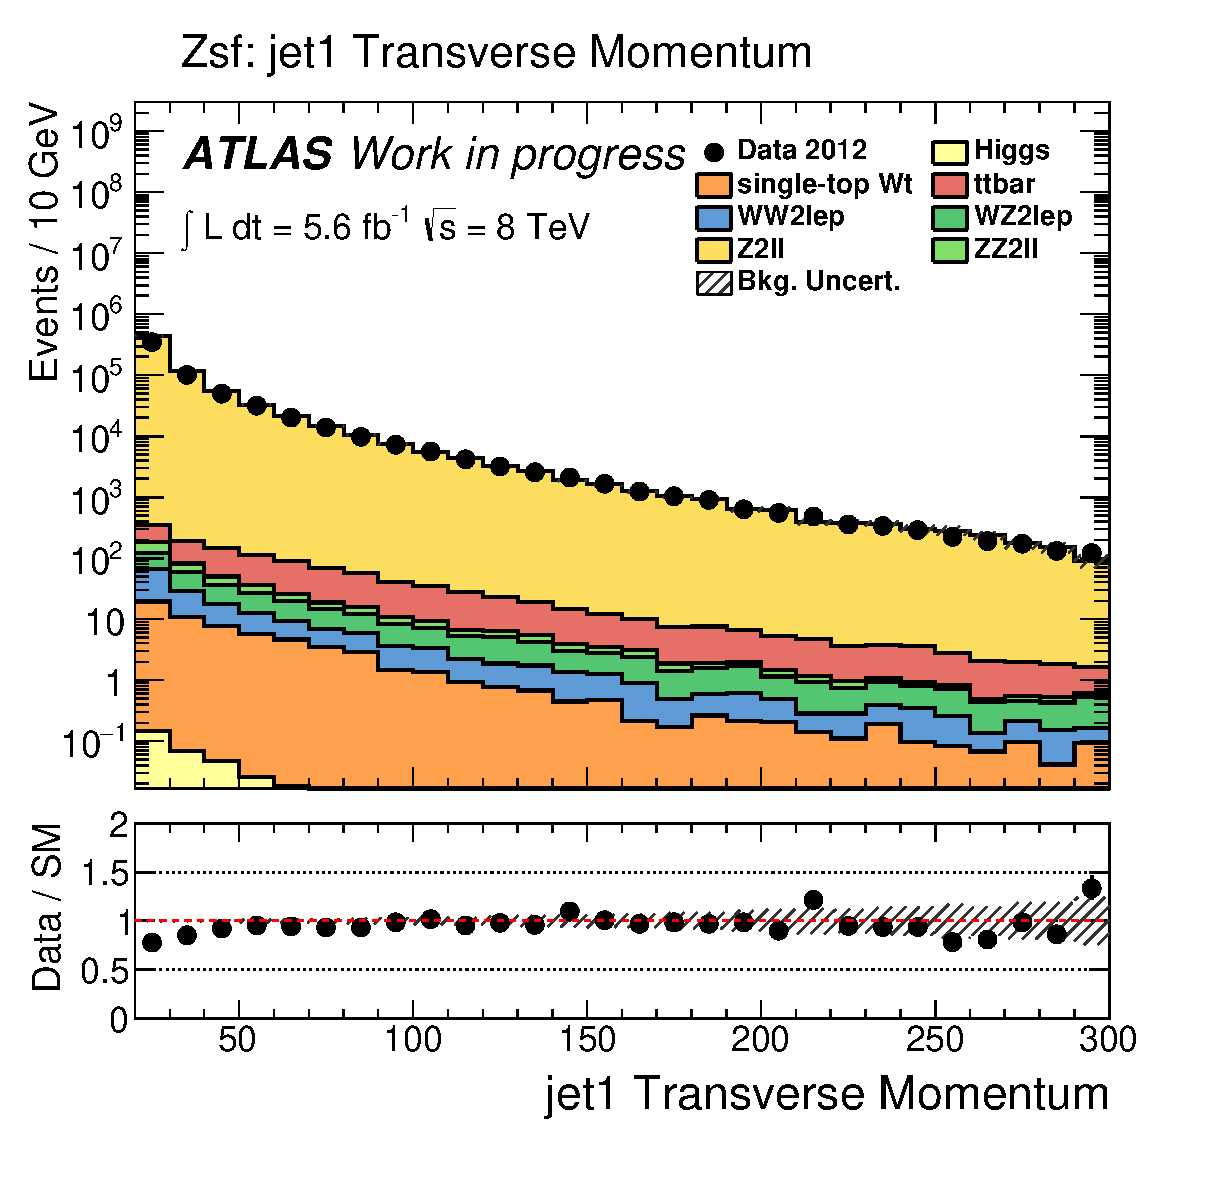
\includegraphics[width=1.0\textwidth]{../scp_landingpad/sf/Zsf_jet1Pt_iso}
			\column{0.25\paperwidth}
				\centering
				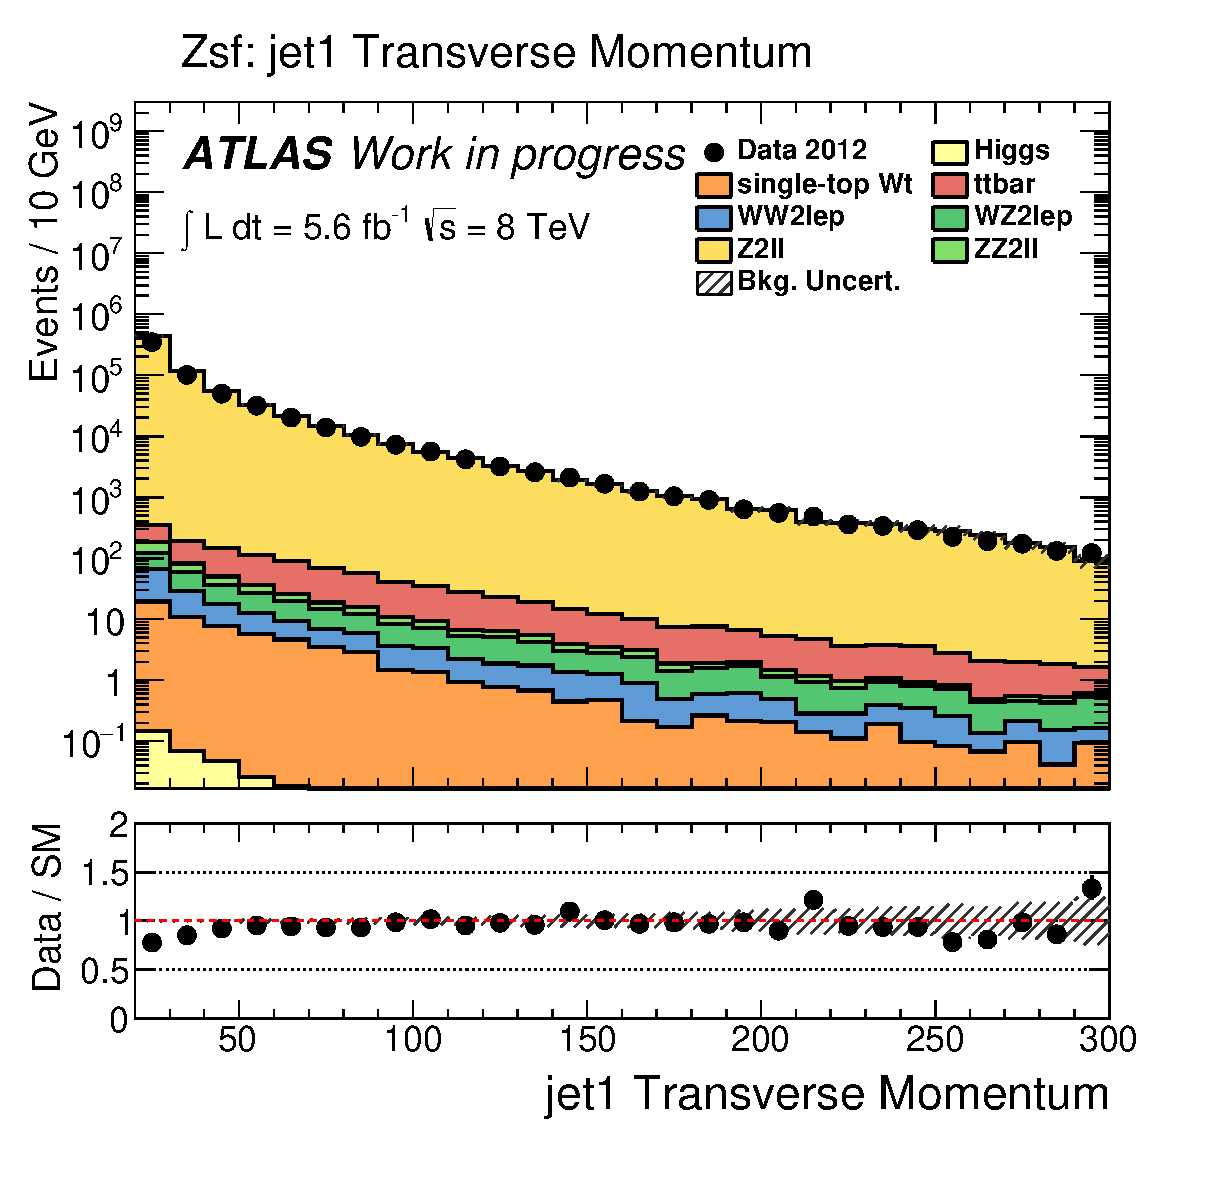
\includegraphics[width=1.0\textwidth]{../scp_landingpad/sf/Zsf_jet1Pt_iso}
			\column{0.25\paperwidth}
				\centering
				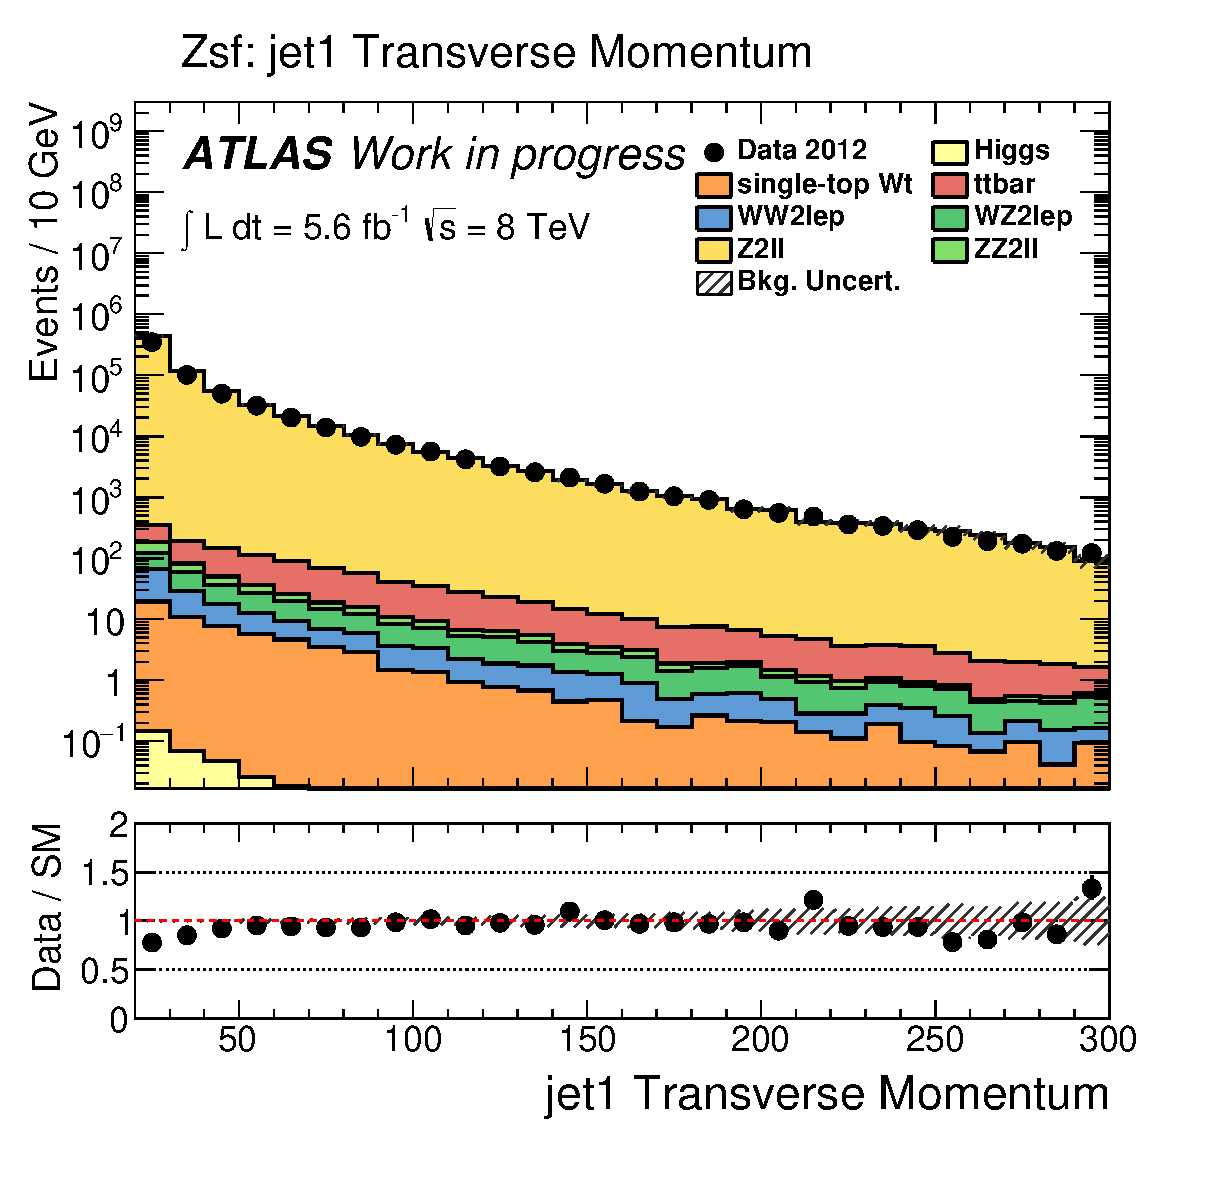
\includegraphics[width=1.0\textwidth]{../scp_landingpad/sf/Zsf_jet1Pt_iso}
			\column{0.25\paperwidth}
				\centering
				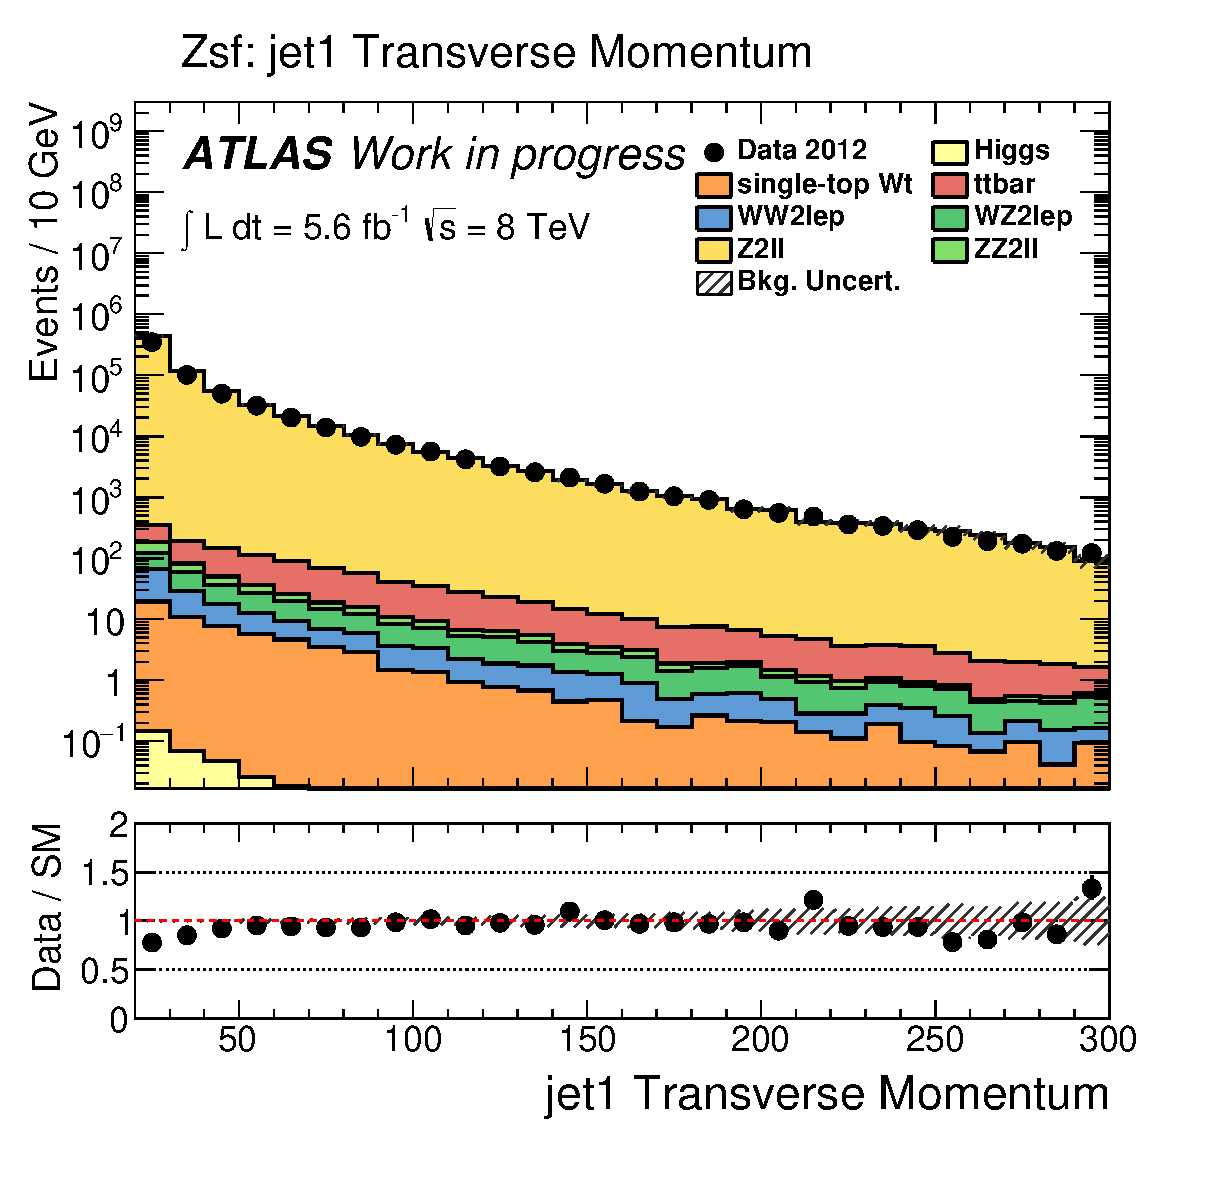
\includegraphics[width=1.0\textwidth]{../scp_landingpad/sf/Zsf_jet1Pt_iso}
		\end{columns}
	\end{block}
	\begin{block}{}  % for upper row of figures
		\begin{columns}[c]
		%	\centering
			\column{0.33\paperwidth}
				\centering
				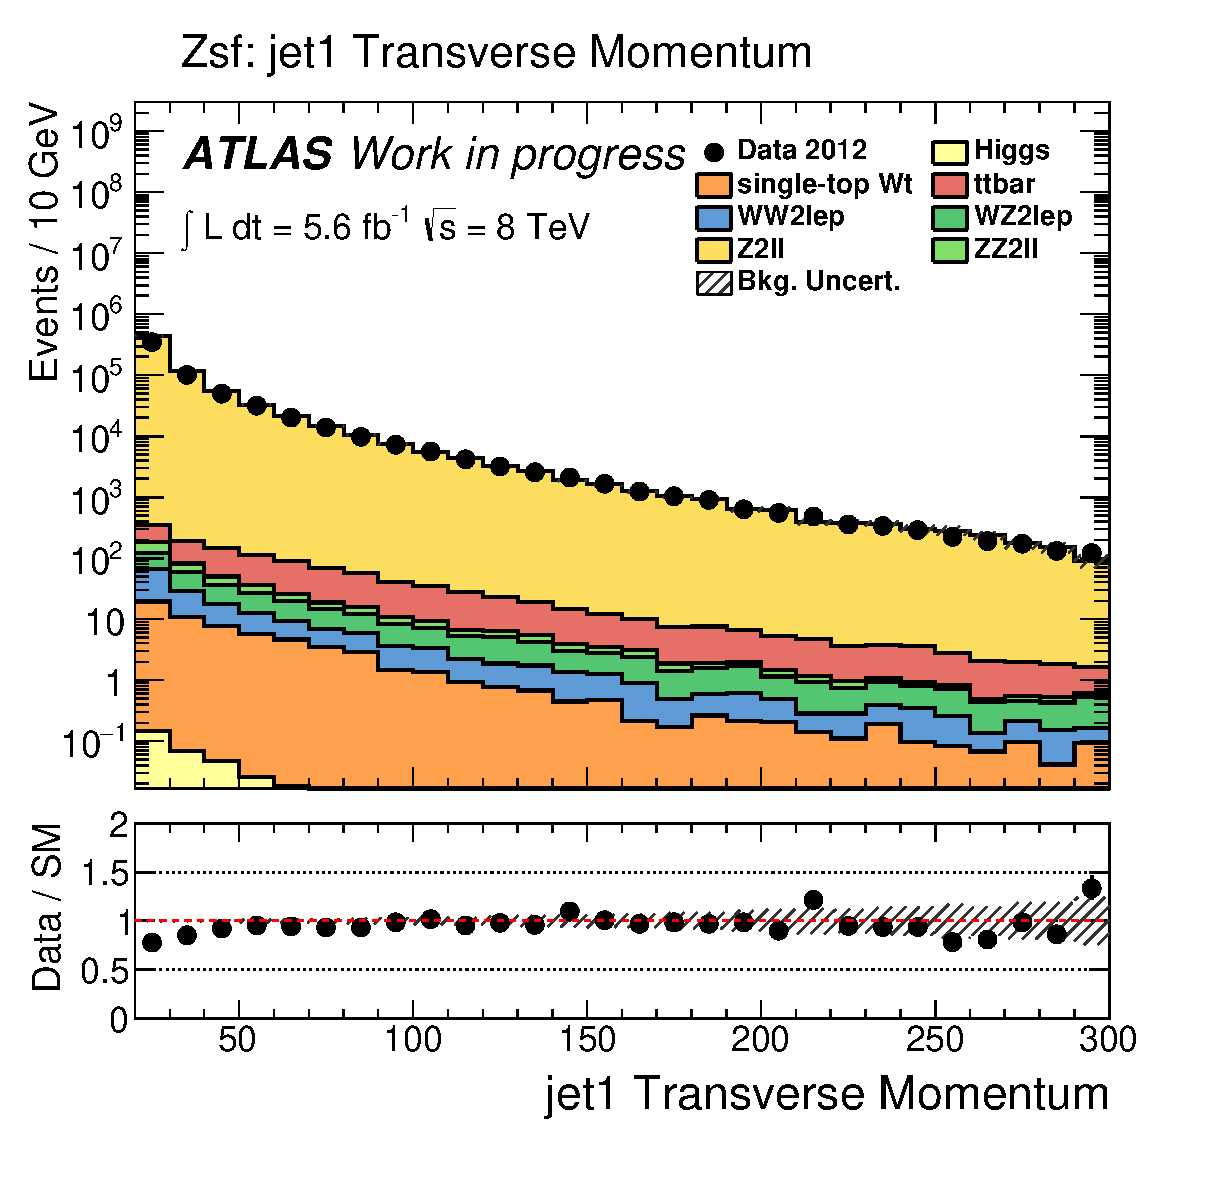
\includegraphics[width=0.95\textwidth]{../scp_landingpad/sf/Zsf_jet1Pt_iso}
			\column{0.33\paperwidth}
				\centering
				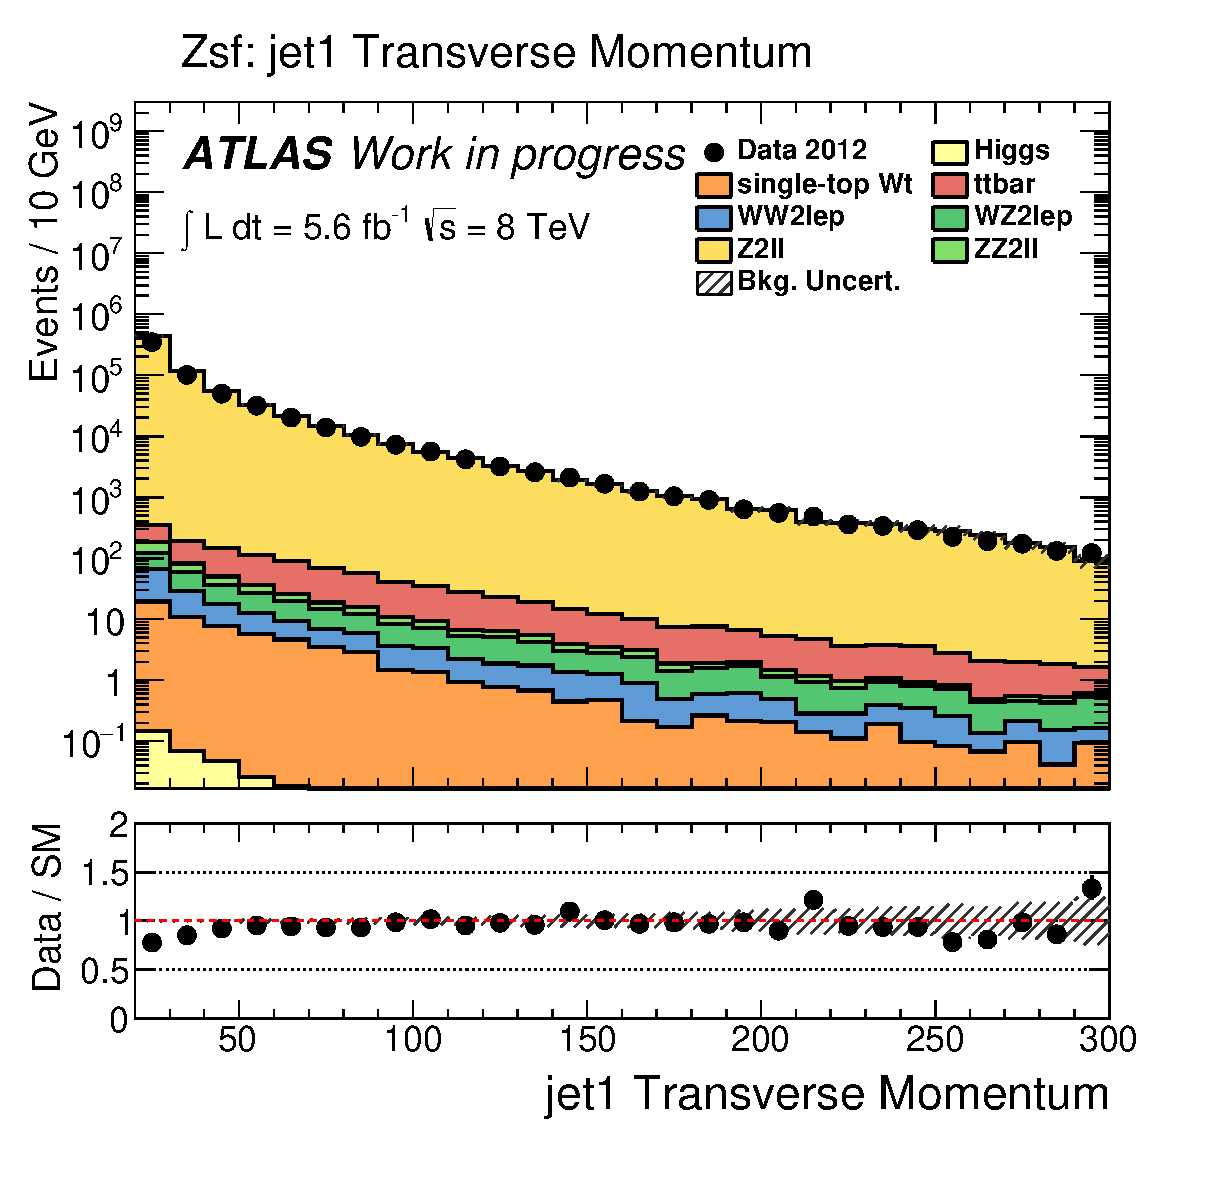
\includegraphics[width=0.95\textwidth]{../scp_landingpad/sf/Zsf_jet1Pt_iso}
			\column{0.33\paperwidth}
				\centering
				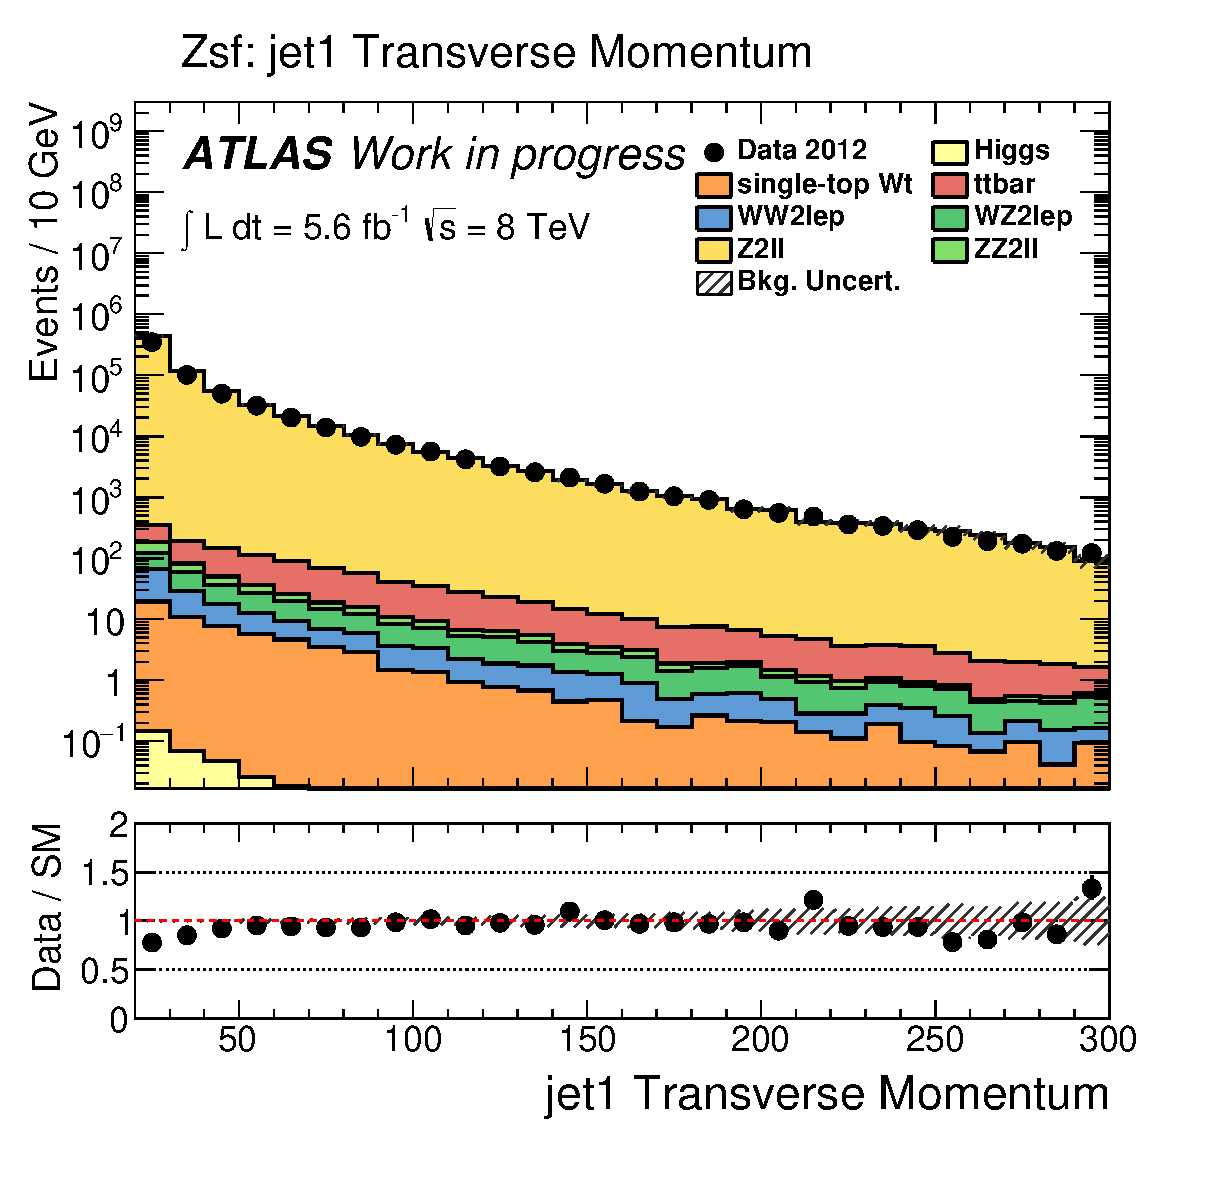
\includegraphics[width=0.95\textwidth]{../scp_landingpad/sf/Zsf_jet1Pt_iso}

		\end{columns}


	\end{block}
\end{frame}
			
				
	


\end{document}